% =============================================================================
% main.tex  —  Documento principal del libro de Fisicoquimica
% =============================================================================
% COMPILACION:
%   pdflatex main.tex
%   makeindex main.idx
%   makeglossaries main
%   bibtex main          (o biber si se usa biblatex)
%   pdflatex main.tex    (segunda pasada para referencias)
%   pdflatex main.tex    (tercera pasada para hipervinculos)
%
% Compatible con Overleaf (compilar con pdfLaTeX, version 2022+)
% =============================================================================

\documentclass[
    11pt,                % Tamano de fuente base
    twoside,             % Impresion a doble cara (margenes alternados)
    openright,           % Cada capitulo inicia en pagina impar
    spanish,             % Idioma principal (usado por algunos paquetes)
]{book}

% -----------------------------------------------------------------------------
% CARGA DEL PREAMBULO COMPLETO
% Todos los \usepackage y configuraciones estan en preamble.tex
% -----------------------------------------------------------------------------
% =============================================================================
% preamble.tex
% Configuracion completa de paquetes y estilos para el libro de Fisicoquimica
% =============================================================================

% -----------------------------------------------------------------------------
% CODIFICACION Y LENGUAJE
% -----------------------------------------------------------------------------
\usepackage[utf8]{inputenc}          % Codificacion de entrada UTF-8
\usepackage[T1]{fontenc}             % Codificacion de fuente T1 (acentos correctos)
\usepackage[spanish,es-nolayout]{babel} % Idioma espanol; es-nolayout evita cambios
                                        % automaticos en listas y teoremas

% Renombrar "Tabla" por "Cuadro" (convencion en ciencias en espanol)
\addto\captionsspanish{%
    \renewcommand{\tablename}{Cuadro}%
    \renewcommand{\listtablename}{\'Indice de cuadros}%
    \renewcommand{\contentsname}{\'Indice de contenidos}%
    \renewcommand{\listfigurename}{\'Indice de figuras}%
    \renewcommand{\figurename}{Figura}%
    \renewcommand{\chaptername}{Cap\'itulo}%
    \renewcommand{\appendixname}{Ap\'endice}%
    \renewcommand{\indexname}{\'Indice alfab\'etico}%
    \renewcommand{\bibname}{Bibliograf\'ia}%
}

% -----------------------------------------------------------------------------
% TIPOGRAFIA: PALATINO
% Newpxtext/newpxmath da Palatino de alta calidad con soporte matematico
% -----------------------------------------------------------------------------
\usepackage{newpxtext}               % Palatino para texto
\usepackage[                         %
    varbb,                           % Usar \mathbb de newpx (no de amssymb)
    varg,                            % Variante de g, y cursivas mas naturales
    amsthm,                          % Integrar con amsthm
]{newpxmath}                         % Palatino para matematicas
\usepackage{microtype}               % Mejora el espaciado tipografico (kerning, etc.)

% -----------------------------------------------------------------------------
% MATEMATICAS Y CIENCIAS
% -----------------------------------------------------------------------------
\usepackage{amsmath}                 % Entornos matematicos avanzados (align, cases...)
% NOTA: amssymb NO se carga explicitamente porque newpxmath ya lo incluye
% internamente. Cargarlo de nuevo provoca el error:
%   "l.261 ...ol{\Bbbk} {\mathord}{AMSb}{"7C}"
% por redefinicion del simbolo \Bbbk del font AMSb.
% Todos los simbolos de amssymb (\mathbb, \mathfrak, etc.) estan disponibles.
\usepackage{amsthm}                  % Entornos de teoremas
\usepackage[version=4]{mhchem}       % Ecuaciones y formulas quimicas: \ce{H2O}
\usepackage{siunitx}                 % Unidades SI: \SI{9.81}{m/s^2}
\DeclareSIUnit\atm{atm}
\DeclareSIUnit\week{semana}
\DeclareSIUnit{\calory}{cal}
\DeclareSIUnit{\year}{yr}
 \DeclareSIUnit\mmHg{mmHg}
 
\sisetup{
    output-decimal-marker = {.},     % Separador decimal: punto
    inter-unit-product = \ensuremath{{}\cdot{}}, % Punto medio entre unidades
    per-mode = symbol,               % Fraccion de unidades con /
    detect-all,                      % Detectar fuente del texto circundante
}
\decimalpoint



% -----------------------------------------------------------------------------
% GRAFICOS Y FIGURAS
% -----------------------------------------------------------------------------
\usepackage{graphics}                % Inclusion basica de graficos
\usepackage[pdftex]{graphicx}                % Inclusion avanzada: [width=], [angle=], etc.
\usepackage{epstopdf}                % Conversion automatica EPS -> PDF
\usepackage{wrapfig}                 % Figuras con texto envolvente (wrapfigure)
\usepackage{float}                   % Control de posicion de flotantes [H]
\usepackage{caption}                 % Personalizar leyendas de figuras y cuadros
\captionsetup{
    font=small,                      % Fuente de caption mas pequena que el texto
    labelfont=bf,                    % "Figura X.Y" en negritas
    labelsep=period,                 % Separador: "Figura 1.1. Titulo"
    skip=6pt,                        % Espacio entre figura y caption
}
\usepackage{subcaption}              % Sub-figuras: (a), (b)...

% Ruta por defecto para buscar figuras
\graphicspath{{figuras/}{../figuras/}}

% -----------------------------------------------------------------------------
% TABLAS
% -----------------------------------------------------------------------------
\usepackage{booktabs}                % Lineas horizontales profesionales: \toprule etc.
\usepackage{tabularx}                % Tablas con columnas de ancho automatico (X)
\usepackage{threeparttable}          % Tablas con notas al pie: \tnote
\usepackage{supertabular}            % Tablas largas que abarcan varias paginas
\usepackage{array}                   % Opciones avanzadas de columnas en tablas
\usepackage{multirow}                % Celdas que abarcan multiples filas

% -----------------------------------------------------------------------------
% DISEÑO DE PAGINA Y ESPACIADO
% -----------------------------------------------------------------------------
\usepackage{geometry}
\geometry{
    paperwidth  = 8in,               % Ancho de pagina: 6 pulgadas
    paperheight = 11in,               % Alto de pagina: 9 pulgadas
    top         = 1in,               % Margen superior
    bottom      = 1in,               % Margen inferior
    inner       = 1in,               % Margen interior (encuadernacion)
    outer       = 0.75in,            % Margen exterior
    includeheadfoot,                 % Incluir encabezado y pie en el calculo
    headheight  = 14pt,              % Altura del encabezado
}
\usepackage{setspace}                % Control de interlineado
\setstretch{1.05}                    % Interlineado ligeramente aumentado (legibilidad)
\usepackage{parskip}                 % Parrafos con espacio vertical en lugar de sangria
\setlength{\parskip}{0.5em}

% -----------------------------------------------------------------------------
% ENCABEZADOS Y PIES DE PAGINA
% -----------------------------------------------------------------------------
\usepackage{fancyhdr}
\pagestyle{fancy}
\fancyhf{}                           % Limpiar todos los campos
\fancyhead[LE]{\small\itshape\leftmark}   % Izquierda paginas pares: capitulo
\fancyhead[RO]{\small\itshape\rightmark}  % Derecha paginas impares: seccion
\fancyfoot[C]{\small\thepage}             % Centro: numero de pagina
\renewcommand{\headrulewidth}{0.4pt}      % Linea bajo el encabezado
\renewcommand{\footrulewidth}{0pt}        % Sin linea en el pie

% Estilo para paginas de inicio de capitulo (plain)
\fancypagestyle{plain}{
    \fancyhf{}
    \fancyfoot[C]{\small\thepage}
    \renewcommand{\headrulewidth}{0pt}
}

% -----------------------------------------------------------------------------
% ESTILOS DE CAPITULO: usando titlesec
% -----------------------------------------------------------------------------
\usepackage{titlesec}
\usepackage{titletoc}

% Formato del titulo de capitulo
\titleformat{\chapter}[display]
    {\normalfont\huge\bfseries\color{chaptercolor}}   % Formato del titulo
    {\chaptertitlename\ \thechapter}                  % Etiqueta "Capitulo N"
    {10pt}                                            % Espacio entre etiqueta y titulo
    {\Huge}                                           % Formato del nombre del capitulo

\titlespacing*{\chapter}{0pt}{-20pt}{30pt}           % Espaciado alrededor del titulo

% Formato de secciones
\titleformat{\section}{\large\bfseries\color{sectioncolor}}{\thesection}{1em}{}
\titleformat{\subsection}{\normalsize\bfseries}{\thesubsection}{1em}{}
\titleformat{\subsubsection}{\normalsize\itshape}{\thesubsubsection}{1em}{}

% -----------------------------------------------------------------------------
% COLORES
% -----------------------------------------------------------------------------
\usepackage{xcolor}
\definecolor{chaptercolor}{RGB}{0, 70, 127}      % Azul marino para titulos de capitulo
\definecolor{sectioncolor}{RGB}{0, 100, 160}     % Azul para secciones
\definecolor{examplecolor}{RGB}{0, 110, 84}      % Verde para ejemplos
\definecolor{exercisecolor}{RGB}{140, 50, 0}     % Cafe para ejercicios
\definecolor{notecolor}{RGB}{180, 100, 0}        % Naranja para notas
\definecolor{linkcolor}{RGB}{0, 70, 127}         % Color de hipervinculos

% -----------------------------------------------------------------------------
% CAJAS Y ENTORNOS ESPECIALES (tcolorbox)
% -----------------------------------------------------------------------------
\usepackage[most]{tcolorbox}
\tcbuselibrary{breakable, skins}

% Entorno: Ejemplo resuelto
\newtcolorbox[auto counter, number within=chapter]{ejemplo}[2][]{%
    enhanced,
    breakable,
    colback  = examplecolor!5,
    colframe = examplecolor,
    fonttitle= \bfseries,
    title    = Ejemplo~\thetcbcounter\ifstrempty{#2}{}{{}: #2},
    label    = ej:\thetcbcounter,
    #1
}

% Entorno: Nota al margen / Nota importante
\newtcolorbox{nota}[1][Nota]{%
    enhanced,
    breakable,
    colback  = notecolor!8,
    colframe = notecolor,
    fonttitle= \bfseries,
    title    = #1,
    left     = 6pt,
    right    = 6pt,
}

% Entorno: Ejercicios (bloque al final de seccion)
\newtcolorbox{bloque_ejercicios}[1][Ejercicios]{%
    enhanced,
    breakable,
    colback  = exercisecolor!5,
    colframe = exercisecolor,
    fonttitle= \bfseries\large,
    title    = #1,
    left     = 8pt,
    right    = 8pt,
    top      = 6pt,
    bottom   = 6pt,
}
% -----------------------------------------------------------------------------
% ENTORNOS DE REACCIONES
%
\makeatletter
\newcounter{reaction}
%%% >> for article <<
%%\renewcommand\thereaction{C\,\arabic{reaction}}
%%% << for article <<
%%% >> for report and book >>
\renewcommand\thereaction{C\,\thechapter.\arabic{reaction}}
\@addtoreset{reaction}{chapter}
%%% << for report and book <<
\newcommand\reactiontag%
  {\refstepcounter{reaction}\tag{\thereaction}}
\newcommand\reaction@[2][]%
  {\begin{equation}\ce{#2}%
  \ifx\@empty#1\@empty\else\label{#1}\fi%
  \reactiontag\end{equation}}
\newcommand\reaction@nonumber[1]%
   {\begin{equation*}\ce{#1}\end{equation*}}
\newcommand\reaction%
  {\@ifstar{\reaction@nonumber}{\reaction@}}
\makeatother
% -----------------------------------------------------------------------------
% ENTORNOS DE TEOREMAS / DEFINICIONES
% -----------------------------------------------------------------------------
\theoremstyle{definition}
\newtheorem{definicion}{Definici\'on}[chapter]
\newtheorem{ley}{Ley}[chapter]
\newtheorem{postulado}{Postulado}[chapter]

\theoremstyle{plain}
\newtheorem{teorema}{Teorema}[chapter]
\newtheorem{corolario}{Corolario}[chapter]

\theoremstyle{remark}
\newtheorem{observacion}{Observaci\'on}[chapter]

% -----------------------------------------------------------------------------
% LISTAS Y ENUMERACIONES
% -----------------------------------------------------------------------------
\usepackage{enumitem}
\setlist[itemize]{noitemsep, topsep=4pt}
\setlist[enumerate]{noitemsep, topsep=4pt}

% Lista de ejercicios numerados
\newlist{ejercicios}{enumerate}{1}
\setlist[ejercicios]{
    label     = \textbf{\arabic*.},
    leftmargin= 2em,
    itemsep   = 6pt,
    topsep    = 4pt,
}

% -----------------------------------------------------------------------------
% GLOSARIO
% -----------------------------------------------------------------------------
\usepackage[
    toc,                             % Agregar glosario al indice de contenidos
    acronym,                         % Seccion separada para acronimos
    style=altlist,                   % Estilo: termino + descripcion en parrafo
    nonumberlist,                    % Sin numeros de pagina en el glosario
]{glossaries}
\newglossary[slg]{symbols}{syi}{syg}{Lista de símbolos}
\makeglossaries
%\setglossarystyle{list}
% -----------------------------------------------------------------------------
% HIPERVINCULOS (hyperref debe ir casi al final del preambulo)
% -----------------------------------------------------------------------------
\usepackage{hyperref}
\hypersetup{
    pdfauthor    = {Dr. José Agustín García Reynoso},
    pdftitle     = {Procesos y Reacciones },
    pdfsubject   = {Atmosf\'ericas},
    pdfkeywords  = {fisicoquímica termodinámica cinética química},
    colorlinks   = true,
    linkcolor    = linkcolor,
    citecolor    = linkcolor,
    urlcolor     = linkcolor,
    bookmarks    = true,
    bookmarksopen= true,
    pdfdisplaydoctitle = true,
    pdfstartview = FitH,
}

\usepackage{bookmark}                % Mejor manejo de bookmarks PDF

% -----------------------------------------------------------------------------
% NUMERACION DE LINEAS (util para revision editorial; comentar en version final)
% -----------------------------------------------------------------------------
\usepackage{lineno}
% Descomentar la siguiente linea para activar numeracion de lineas:
% \linenumbers

% -----------------------------------------------------------------------------
% DIAGRAMAS CON EPIC (entornos picture extendidos)
% -----------------------------------------------------------------------------
\usepackage{epic}                    % Extiende el entorno picture de LaTeX

% -----------------------------------------------------------------------------
% REFERENCIAS Y CITAS
% -----------------------------------------------------------------------------
\usepackage[numbers, sort&compress]{natbib}  % Referencias numeradas y comprimidas
\bibliographystyle{achemso}          % Estilo ACS (quimica); cambiar segun editorial

% -----------------------------------------------------------------------------
% INDICE ANALITICO
% -----------------------------------------------------------------------------
\usepackage{makeidx}
\makeindex

% -----------------------------------------------------------------------------
% UTILIDADES GENERALES
% -----------------------------------------------------------------------------
\usepackage{xspace}                  % Espaciado inteligente despues de macros
\usepackage{ifthen}                  % Condicionales en LaTeX
\usepackage{calc}                    % Calculos aritmeticos en LaTeX
\usepackage{etoolbox}                % Herramientas de programacion LaTeX

% -----------------------------------------------------------------------------
% MACROS DE CONVENIENCIA
% Atajos para simbolos y unidades frecuentes en fisicoquimica
% -----------------------------------------------------------------------------

% Constantes fisicas (valor + unidad en formato siunitx)
\newcommand{\NA}{\ensuremath{N_{\!A}}\xspace}    % Numero de Avogadro
\newcommand{\kb}{\ensuremath{k_B}\xspace}         % Constante de Boltzmann
\newcommand{\Rgas}{\ensuremath{R}\xspace}         % Constante universal de los gases
\newcommand{\hplanck}{\ensuremath{h}\xspace}      % Constante de Planck

% Notacion de derivadas
\newcommand{\dif}{\mathop{}\!\mathrm{d}}          % Diferencial: d (redondo)
\newcommand{\Dif}{\mathop{}\!\mathrm{D}}          % Derivada funcional
\newcommand{\pder}[2]{\frac{\partial #1}{\partial #2}}   % Derivada parcial
\newcommand{\der}[2]{\frac{\dif #1}{\dif #2}}            % Derivada total

% Notacion termodinamica
\newcommand{\DeltaH}{\ensuremath{\Delta H}\xspace}
\newcommand{\DeltaG}{\ensuremath{\Delta G}\xspace}
\newcommand{\DeltaS}{\ensuremath{\Delta S}\xspace}
\newcommand{\Keq}{\ensuremath{K_{\text{eq}}}\xspace}
\newcommand{\stdstate}{\ensuremath{^{\circ}}\xspace}  % Superindice de estado estandar

% Abreviaciones utiles
\newcommand{\eg}{e.g.\xspace}
\newcommand{\ie}{i.e.\xspace}
\newcommand{\etal}{\textit{et al.}\xspace}

%%%%% Problem Set Macros

% =============================================================================
% FIN DE preamble.tex
% =============================================================================


% -----------------------------------------------------------------------------
% CARGA DEL GLOSARIO
% Los terminos se definen en glossary/glosario.tex
% -----------------------------------------------------------------------------
\input{glossary/glosario}
\includeonly{chapters/cap08_PQatmos} 
% =============================================================================
%  INICIO DEL DOCUMENTO
% =============================================================================
\begin{document}
\newcounter{cm}
\setlength{\unitlength}{1mm}
\newcolumntype{Y}{>{\centering\arraybackslash}X}%
% ---- Fuente de encabezados: nombre de capitulo y seccion en minusculas ------
\renewcommand{\chaptermark}[1]{\markboth{\chaptername\ \thechapter.\ #1}{}}
\renewcommand{\sectionmark}[1]{\markright{\thesection\ #1}}
% lado a lado
\long\def\sidebyside#1#2{%
\hbox to\textwidth{\vtop{\hsize=.5\textwidth%
\advance\hsize by -.5\columnsep
\parindent=0pt
\centering
 
#1\vskip1sp}\hskip\columnsep\vtop{\hsize=.5\textwidth%
\advance\hsize by -.5\columnsep
\parindent=0pt
\centering
#2

}\hfill}}
% =============================================================================
%  PORTADA
% =============================================================================
\begin{titlepage}
    \thispagestyle{empty}
    \centering

    \vspace*{1.5cm}

    % Logotipo institucional (opcional)
     
\includegraphics[width=4cm]{CCA.png}\\[1cm]

    {\color{chaptercolor}\rule{\linewidth}{2pt}}\\[0.6cm]

    {\Huge\bfseries\color{chaptercolor}
        Procesos y Reacciones\\[0.3cm]
        Atmosf\'ericas
    }\\[0.5cm]

    {\color{chaptercolor}\rule{\linewidth}{2pt}}\\[1.2cm]

    {\LARGE\itshape Termodin\'amica, Cin\'etica Qu\'imica}\\[0.3cm]
    {\Large\itshape y Equilibrio}\\[2cm]

    {\large\bfseries Dr. José Agustín García Reynoso}\\[0.3cm]
    {\normalsize UNAM / Instituto de Ciencias de la Atmósfera y Cambio Climático }\\[0.2cm]
    {\normalsize agustin@atmosfera.unam.mx}\\[2.5cm]

    {\large Primera edici\'on}\\[1cm]

    \vfill

    {\large\bfseries Universidad Nacional Autónoma de México}\\[0.2cm]
    {\normalsize Ciudad de M\'exico, 2025}

\end{titlepage}

% =============================================================================
%  PAGINA DE COPYRIGHT
% =============================================================================
\thispagestyle{empty}
\vspace*{\fill}
\noindent
\textbf{T\'itulo:} Procesos y Reacciones en la Atm\'osfera: Termodin\'amica, Cin\'etica Qu\'imica y Equilibrio\\[0.4em]
\textbf{Autor:} Dr. José Agustín García Reynoso\\[0.4em]
\textbf{Primera edici\'on}\\[1.5em]

\noindent
\copyright\ 2026 José Agustín García Reynoso. Todos los derechos reservados.\\[0.5em]

\noindent
Ninguna parte de esta publicaci\'on puede ser reproducida, almacenada en un sistema de recuperaci\'on de datos ni transmitida en ninguna forma ni por ning\'un medio, electr\'onico, mec\'anico, fotocopia, grabaci\'on ni cualquier otro, sin el permiso previo por escrito del titular del copyright.\\[1em]

\noindent
\textbf{ISBN:} 978-XX-XXXX-XXX-X\\[0.3em]
\textbf{DOI:} \url{https://doi.org/XX.XXXX/XXXXX}\\[1.5em]

\noindent
Impreso en M\'exico / Printed in Mexico\\[0.3em]

\noindent
\textit{Dise\~no de portada:} Nombre del dise\~nador\\
\textit{Composici\'on tipogr\'afica}: \LaTeX{}
\clearpage

% =============================================================================
%  PAGINAS PRELIMINARES (numeracion romana)
% =============================================================================
\frontmatter                         % Numeracion romana: i, ii, iii...
\pagestyle{fancy}

% ---- Prefacio ---------------------------------------------------------------
\chapter*{Prefacio}
\addcontentsline{toc}{chapter}{Prefacio}

Dentro del \'area en Ciencias de la Tierra se recibe una gran diversidad de estudiantes que provienen de diferentes campos del conocimiento. Si bien muchos de ellos estudiaron y revisaron durante el bachillerato parte de los temas que aqu\'{\i} se presentan, \'estos no son revisados dentro de sus respectivas carreras profesionales. El motivo de este trabajo es ayudar  a recordar y a presentar los temas relacionados a la fisicoqu\'{\i}mica atmosf\'erica que sean \'utiles para el desarrollo de sus estudios en el posgrado.

 En la primera parte se presentan los temas fundamentales de la termodin\'amica, con base en las leyes de la termodin\'amica, energ\'{\i}a libre, reacciones en los seres vivos. Posteriormente se abordan los temas de procesos electroqu\'{\i}micos donde se ven los fen\'omenos de \'oxido-reducci\'on, los sistemas electroqu\'{\i}micos y la corrosi\'on.
 
 Si bien la termodin\'amica nos indica la espontaneidad de un proceso, lo anterior no nos indica la rapidez con la que se puede dar, por lo que se abordan los temas de cin\'etica qu\'{\i}mica, teor\'{\i}a de colisiones, energ\'{\i}a de activaci\'on  y los factores que influyen en la rapidez de una reacci\'on.
 
 En la parte de equilibrio qu\'{\i}mico se aborda el tema reversibilidad de las reacciones, la constante de equilibrio y algunas aplicaciones de la misma con el $p$H.
 
 En la parte de qu\'{\i}mica org\'anica se hace una descripci\'on de los niveles de energ\'{\i}a en los \'atomos, las configuraciones electr\'onicas, los s\'{\i}mbolos de Lewis, lo que es la energ\'{\i}a de ionizaci\'on. Se muestran las familias de compuestos org\'anicos basados en el n\'umero de enlaces entre \'atomos de carbono y con otros elementos como el ox\'{\i}geno y el nitr\'ogeno.
 
 En la segunda parte se muestran los compuestos considerados como contaminantes y su clasificaci\'on, el manejo de unidades de los mismos y los procesos fisicoqu\'{\i}micos  en la atm\'osfera en los que \'estos intervienen.
 
 Si el lector desea profundizar en  alg\'un tema se presenta la bibliograf\'{\i}a complementaria a los temas tratados.
 
 Se espera que sea un libro texto para aquellos quienes los temas de qu\'{\i}mica son poco estudiados dentro de sus formaci\'on profesional.
 

En el texto se emplea el sistema de unidades SI (Sistema Internacional de Unidades)  sin embargo existen ejemplos y ejercidos que se expresan en unidades inglesas.



\medskip
\noindent
Se recomienda que el lector tenga conocimientos previos de:
\begin{itemize}
    \item C\'alculo diferencial e integral (una y varias variables)
    \item \'Algebra lineal
    \item Qu\'imica general y org\'anica a nivel licenciatura
    \item F\'isica b\'asica (termodin\'amica cl\'asica)
\end{itemize}

\medskip
\noindent
Cada cap\'itulo incluye \textbf{ejemplos resueltos} detallados y un conjunto de
\textbf{ejercicios propuestos} al final. Las respuestas a los ejercicios seleccionados
se encuentran en el ap\'endice.

\medskip
\noindent
\textit{Ciudad de M\'exico, 2026}\\[0.5em]
\textit{Dr. José Agustín García Reynoso}

% ---- Indice de contenidos ---------------------------------------------------
\tableofcontents

% ---- Indice de figuras ------------------------------------------------------
\listoffigures

% ---- Indice de cuadros ------------------------------------------------------
\listoftables

% =============================================================================
%  CUERPO PRINCIPAL DEL LIBRO (numeracion arabiga)
% =============================================================================
\mainmatter                          % Numeracion arabiga: 1, 2, 3...
\pagestyle{fancy}

% ---- PARTE I ----------------------------------------------------------------
\part{Termodin\'amica Qu\'imica}

\chapter[Energ\'{\i}a y reacciones]{La energ\'{\i}a y las reacciones qu\'{\i}micas}

El estudio de la energ\'{\i}a y las reacciones qu\'{\i}micas es fundamental para comprender los procesos que rigen tanto la naturaleza como las aplicaciones tecnol\'ogicas. Este cap\'{\i}tulo explora los principios b\'asicos de la termodin\'amica, la electroqu\'{\i}mica y la termoqu\'{\i}mica, proporcionando una base s\'olida para entender c\'omo la energ\'{\i}a se transforma y se transfiere en los sistemas qu\'{\i}micos.

En la \textbf{Secci\'on 1.1}, se introduce el concepto de \textbf{energ\'{\i}a} y su relaci\'on con las reacciones qu\'{\i}micas. Esta parte se inicia con el desarrollo de la noci\'on de sistema, estados y funciones de estado. Se analizan los tipos de sistemas, las propiedades de un sistema y los cambios de estado, junto con el comportamiento de los gases ideales y no ideales, las ecuaciones de estado y la Ley General de los Gases. Adem\'as, se interpreta el significado de la primera ley de la termodin\'amica, expresada como $\Delta E = q + w$, que establece la conservaci\'on de la energ\'{\i}a. Se establece la diferencia entre energ\'{\i}a interna y entalp\'{\i}a, y se clasifican las reacciones en exot\'ermicas y endot\'ermicas.

En la \textbf{Secci\'on 1.2}, se estudia la forma en que se presentan gr\'aficamente los cambios de energ\'{\i}a asociados a los cambios qu\'{\i}micos, as\'{\i} como la relaci\'on entre las entalp\'{\i}as de reacci\'on y las energ\'{\i}as de enlace. Se definen los estados est\'andares y se explica c\'omo las entalp\'{\i}as de formaci\'on y la Ley de Hess se aplican en c\'alculos termoqu\'{\i}micos. Estos conceptos permiten comprender y predecir los cambios energ\'eticos en reacciones qu\'{\i}micas complejas.

En la \textbf{Secci\'on 1.3}, se introduce el concepto de \textbf{entrop\'{\i}a} ($\Delta S$), una medida del desorden en un sistema, y su relaci\'on con los cambios de energ\'{\i}a en transformaciones f\'{\i}sicas y qu\'{\i}micas. Se interpreta y aplica la ecuaci\'on que relaciona energ\'{\i}a libre, entalp\'{\i}a y entrop\'{\i}a: $\Delta G = \Delta H - T \Delta S$. Se analiza la importancia de la variaci\'on de la energ\'{\i}a libre durante un cambio qu\'{\i}mico como criterio para predecir, sin necesidad de experimentos, si un proceso puede ocurrir o no. Finalmente, se estudia la relaci\'on entre la energ\'{\i}a libre, los procesos espont\'aneos y las reacciones exerg\'onicas y enderg\'onicas.

La \textbf{Secci\'on 1.4} aborda los \textbf{procesos electroqu\'{\i}micos}, incluyendo las reacciones de oxidaci\'on-reducci\'on, las celdas electroqu\'{\i}micas (galv\'anicas y electrol\'{\i}ticas), los sistemas electroqu\'{\i}micos y el potencial est\'andar de reducci\'on. Tambi\'en se discuten temas relacionados con la corrosi\'on de metales y las estrategias para su prevenci\'on.

Este cap\'{\i}tulo proporciona una visi\'on integral de los principios energ\'eticos y qu\'{\i}micos que rigen los procesos naturales y tecnol\'ogicos, sentando las bases para su aplicaci\'on en diversos campos de la ciencia y la ingenier\'{\i}a.

\section{Sistemas, estados y funciones de estado}
\index{sistema}
 Un \textit{\gls{sistema} termodin\'a\-mi\-co} es una porci\'on del universo separada por fronteras que nos interesa estudiar, tambi\'en se puede definir como la parte del universo f\'{\i}sico cuyas propiedades se est\'an investigando. El sistema est\'a confinado a un lugar definido en el espacio por la \gls{frontera}\index{sistema!frontera} que lo separa del resto del universo (el medio exterior). La ciencia que estudia c\'omo la energ\'{\i}a y propiedades medibles de un sistema se relacionan y la interacci\'on con los alrededores es la \textbf{\gls{termodinamica}} \index{termodinamica@termodin\'amica} su nombre procede del griego \textit{termos} (calor) y \textit{dinamos} (movimiento). Es parte de la f\'{\i}sica que trata del estudio de los procesos en los que se transfiere energ\'{\i}a o sus manifestaciones como calor y como trabajo. 

\subsection{Tipos de sistemas}

\index{sistema!tipos}
\begin{itemize}
\item \textit{Aislado} cuando la frontera evita cualquier interacci\'on con la materia o  energ\'{\i}a del exterior.
\item \textit{Abierto} cuando pasa materia a trav\'es de la frontera.
\item \textit{Cerrado} aquel que no intercambia materia con sus alrededores pero s\'{\i} energ\'{\i}a.
\item \textit{Homog\'eneo} cuando contiene \'unicamente una fase.
\item \textit{Heterog\'eneo} contiene m\'as de una fase.
\end{itemize}

Se define a una \gls{fase}\index{sistema!fase} como una porci\'on homog\'enea del sistema, f\'{\i}sica\-mente diferenciable y separable mec\'anicamente. Si el sistema ``agua'' coexisten las tres formas s\'olida (hielo), l\'{\i}quida y gaseosa (vapor), cada una constituye una fase separada de las otras por un l\'{\i}mite.


\subsection{Propiedades de un sistema}
Las propiedades de un sistema\index{sistema!propiedades} son los atributos f\'{\i}sicos que perciben los sentidos directamente o con un m\'etodo experimental. La presi\'on y el volumen son propiedades f\'acilmente perceptibles a las que se les designa un valor num\'erico. La entalp\'{\i}a es una propiedad que s\'olo se detecta con un experimento y no se mide su valor absoluto sino sus cambios.

Las propiedades del sistema se dividen en dos clases:

\begin{itemize}
\item \textit{Intensivas} \index{propiedades!intensivas} son aquellas las cuales no dependen de la cantidad de substancia o del tama\~no del  sistema, por lo que su valor permanece inalterable al subdividir el sistema inicial en varios subsistemas. Entre estas propiedades se encuentra la densidad (\gls{densidad}), el \'{\i}ndice de refracci\'on, la masa molar, el volumen molar y la e\-nerg\'{\i}a molar. 
\item \textit{Extensivas} \index{propiedades!extensivas}son aquellas que si dependen de la cantidad de sustancia o del tama\~no de un sistema, son magnitudes cuyo valor es proporcional al tama\~no del sistema que describe, dependen de dos de las tres variables presi\'on ($P$), volumen ($V$) y temperatura ($T$) y el n\'umero de moles.
\end{itemize}

\subsection{Estado de un sistema}
\index{sistema!estado}
Un sistema se encuentra en un estado definido cuando cada una de sus propiedades tiene un valor determinado. Debemos saber que con base en el estudio experimental del sistema o de la experiencia con sistemas semejantes, qu\'e propiedades deben considerarse, con el fin de que el estado del sistema sea definido con precisi\'on suficiente para el prop\'osito buscado.

\begin{ejemplo}{Estado de un sistema}
El estado est\'andar del agua l\'{\i}quida a \SI{25}{\celsius} y \SI{1}{\bar}\footnotemark.
\end{ejemplo}
 \footnotetext{La \gls{IUPAC} con base en el trabajo del Comit\'e de Datos para la ciencia y Tecnolog\'{\i}a (\gls{codata}) recientemente recomend\'o que el estado est\'andar se refiera a la presi\'on de \SI{1}{\bar}  (\SI{100 000}{\pascal}). La diferencia entre una atm\'osfera y un bar es de alrededor de 1\% .}
 
 El estado est\'andar se describe con un cero como super\'{\i}ndice, por ejemplo $\Delta H^\circ$. Este s\'{\i}mbolo expresa en los textos que siguen la convenci\'on antigua, que los valores corresponden a  la presi\'on de 1 atm\'osfera.

\subsection{Cambio de estado, trayectoria, ciclo, proceso}

Sometamos a un sistema a un cambio de estado \index{sistema!cambio de estado} desde
condiciones espec\'{\i}ficas iniciales hasta condiciones espec\'{\i}ficas finales.

El \textit{cambio de estado}\index{estado!cambio} est\'a completamente  definido cuando se especifica el estado inicial y el estado final.

La \textit{trayectoria} \index{estado!trayectoria} del cambio de estado se define especificando el estado inicial, la secuencia de estados intermedios que va tomando el sistema y el estado final.

Un \textit{proceso} \index{proceso} es el m\'etodo de operaci\'on mediante el cual se realiza un cambio de estado. La descripci\'on de un proceso consiste en establecer todo o parte de los siguientes: (1) la frontera; (2) cambio de estado, la trayectoria o los efectos producidos en el sistema durante cada etapa del proceso y (3) los efectos producidos en el medio externo durante cada etapa del proceso.

Supongamos que un sistema sometido a un cambio de estado regrese a su estado inicial. La trayectoria de esta transformaci\'on c\'{\i}clica se llama ciclo y el proceso mediante el cual se realiz\'o la transformaci\'on se llama \textit{proceso c\'{\i}clico}.

Una \textit{\gls{variabledeestado}} \index{estado!variable} es aquella que tiene un
valor definido cuando especifica el estado de un sistema.

En la siguiente parte se mostrar\'an los conceptos para poder responderse a preguntas tales como: ?`Qu\'e es un sistema?, ?`D\'onde existe una frontera?, ?`Cu\'al es el estado inicial?, ?`Cu\'al es el estado final?, ?`Cu\'al es la trayectoria de transformaci\'on?.


\subsection{Gases ideales} 
Los \gls{gasesideales}\index{gases ideales} son aquellos cuyo comportamiento no se
altera por fuerzas de cohesi\'on y vol\'umenes moleculares. Los \gls{gasesreales}
est\'an m\'as cercanos al comportamiento ideal mientras m\'as bajas sean las
presiones y m\'as altas las temperaturas.

\subsection{Ecuaciones de estado}

Las ecuaciones\index{estado!ecuaciones}  que representan las relaciones presi\'on
(\gls{presion})- volumen (\gls{volumen}) -
temperatura(\gls{temperatura}) de los gases se conocen como \gls{ecuaciondeestado}, ya que describen completamente el estado de cualquier
sistema gaseoso. Las variables de estas ecuaciones se dividen en dos clases:
moles (\gls{moles}) y $V$ son variables extensivas (propiedades que dependen de la
cantidad de material) mientras que $P$ y $T$ son intensivas.

\begin{figure}[ht]

\begin{center}
\begin{tabular}{||c|c|c|c|c|c||} \hline \hline
      &           &          &           &  & \\ \hline
      &           &          &           &  & \\ \hline
      &           &          &           &  & \\ \hline
      &           &          &           &  & \\ \hline
      &           &          &           &  &  \\ \hline \hline
\end{tabular}
\caption{Subdivisi\'on del sistema}
\label{fig:1}
\end{center}
\end{figure}


El valor de cualquier propiedad extensiva\index{estado!propiedad extensiva} se obtiene sumando
los va\-lores de la misma en todas partes del sistema. Supongamos que el sistema est\'a
subdividido en muchas partes peque\~nas, como en la Figura~\ref{fig:1}, entonces el volumen total del sistema se obtiene sumando los vol\'umenes de
cada una de las partes.

Las propiedades intensivas\index{estado!propiedad intensiva} no se obtienen mediante tal
proceso de su\-ma, sino que se miden de cualquier punto del sistema y cada una tiene un valor
uniforme en cualquier punto del sistema en equilibrio; por ejemplo, $T$ y $P$.

La temperatura ($T$) en todas las ecuaciones de estado es la \index{temperatura!absoluta} \gls{temperaturaabsoluta} es decir para el sistema m\'etrico decimal se encuentra en Kelvin\footnotemark{ Es importante identificar que la abreviatura K de Kelvin es en may\'uscula mientras que de kilo (k) es en min\'uscula. As\'{\i} Kg representa Kelvin gramo y kg es kilogramo.} .

\begin{equation}
T[\si{\kelvin}]_{absoluta} = T[\si{\celsius}] + \SI{273.15}{\kelvin}
\end{equation}

\textit{Ley de \gls{boyle}} \index{Boyle@\textbf{Boyle}!Ley de} Siempre que la masa
y la temperatura de una muestra de gas se mantienen constantes, el volumen del gas es
inversamente proporcional a su presi\'on absoluta.
\begin{equation}
P \propto \frac{1}{V} \quad{ \longrightarrow }\quad  P = \frac{k}{V}
\end{equation}
Tambi\'en podemos escribirla de la siguiente manera:
\begin{equation}
P_1 V_1 = P_2 V_2
\end{equation}
\begin{ejemplo}{Ley de Boyle}
 Un gas se comprime isotermicamente de $P_1=  \SI{1}{\bar}$  y  $V=  \SI{10}{\liter}$  a una presi\'on de  \SI{2}{ \bar}. ?`Cu\'al es su volumen?\\[3pt]

$V_2 = \frac{P_1 V_1}{P_2}$\hskip.3in substituyendo\hskip.3in  $V_2 = \frac{ \SI{1}{\bar}( \SI{10}{\liter})}{ \SI{2}{\bar}} =  \SI{5}{\liter}$
\end{ejemplo}

\textit{Ley de \gls{charles}}\index{Charles@\textbf{Charles}} Siempre que la masa y la presi\'on de una muestra de gas se mantienen constantes, el volumen de la muestra es directamente proporcional a su temperatura absoluta.
\begin{equation}
V= k'T
\end{equation}
que tambi\'en se puede escribir de la siguiente forma:
\begin{equation}
\frac{V_1}{T_1} = \frac{V_2}{T_2}
\end{equation}

\begin{ejemplo} {Ley de Charles}
 A un gas ideal se le incrementa la temperatura a presi\'on constante de T = \SI{15}{\celsius} a \SI{125}{\celsius} si su volumen inicial es de \SI{100}{\liter}. ?`Cu\'al es su volumen final?. \vskip0.1in
Para convertir la temperatura a absoluta se suman \SI{273.15}{\kelvin} as\'{\i} tenemos que \SI{15}{\celsius} son   \SI{288.15}{\kelvin} y  \SI{125}{\celsius}  \SI{398.15}{\kelvin}
\vskip.2in
${V_2} = \frac{V_1 \times T_2}{T_1}$\hskip.25in sustituyendo\hskip.25in 
$V_2 = \frac{\SI{100}{\liter} \times \SI{398.15}{\kelvin}}{\SI{288.15}{\kelvin}} = \SI{138.17}{\liter}$
\end{ejemplo}\vskip0.1in

\textit{Ley combinada de los gases} \index{ley combinada de los gases}. Empleando las ecuaciones anteriores se puede obtener la siguiente realci\'on entre el volumen, presi\'on y temperatura:
\begin{equation}
\frac{P_1V_1}{T_1} = \frac{P_2V_2}{T_2}
\end{equation}

 
 \subsection{Ley General de los gases}
 \index{ley!general de los gases}
 La ley general de los gases se puede aplicar para las condiciones de presi\'on y temperatura ambiente. La relaci\'on que guarda la temperatura, presi\'on, volumen y cantidad de masa se muestra en la siguiente ecuaci\'on:

\begin{equation}
PV = nRT\label{lgg}
\end{equation}

donde :

\qquad\begin{tabular}{c@{ -- }ll}
$P$ & presi\'on &[atm]\\
$V$ & volumen &[\si{\liter}]\\
$n$ & moles de gas &[\si{\gram\mole}]\\
\gls{constR} & Constante de los gases & [\si{\liter\atm\per\mole\per\kelvin}] \index{constante!ley general de los gases}\\
$T$ & temperatura absoluta&[\si{\kelvin}]\\
\end{tabular}

\begin{ejemplo}{Volumen para un gas ideal}
\label{ej:gas_ideal}
?`Cu\'al es el volumen que ocupan 112 g de Nitr\'ogeno (N$_2$) a la presi\'on de la Ciudad de M\'exico (0.77 atm) y a una temperatura de \SI{15}{\celsius} . (R = 0.082057 \si{\liter\atm\per\mole\per\kelvin})%


Convirtiendo los \SI{15}{\celsius}  a absoluta tenemos \SI{288.15}{\kelvin}

Moles de N$_2$ = $\frac{\SI{112}{ \gram}}{\SI{28}{\gram\per\mole}} =$ \SI{4}{\mole}

$V = \frac{nRT}{P}$
 substituyendo
  $V =
 \frac{\SI{4}{\mole} \times 0.082057\si{\liter\atm\per\mole\per\kelvin} \times \SI{288}{\kelvin}} {\SI{0.77}{\atm}}$\vskip0.1in

$V = \SI{122.7}{\liter}$
\end{ejemplo}

y a partir de la \textbf{Ec.~\ref{lgg}} se puede despejar los t\'erminos para calcular la densidad de un gas mediante la siguiente ecuaci\'on :
\index{densidad!c\'alculo}
\begin{equation}
\rho = \frac{PM}{RT}
\label{ecdensidad}
\end{equation}

\begin{tabular}{llll}
Donde:\\
&\gls{densidad} & Densidad del gas & [\si{\kilo\gram\per\cubic\metre}]\\
&$P$ & presi\'on   &[atm]\\
&$M$ & Peso molecular del gas&[g/gmol]\\
&$R$ & Constante de los gases& [\si{\liter\atm\per\mole\per\kelvin}] \\
&$T$ & Temperatura  &[\si{\kelvin}] \\
\end{tabular}

\begin{ejemplo}{Ley general de los gases}%
\label{ej:gas_ideal2}
 Calcular la densidad de un gas cuyo peso molecular es 29.98 g/gmol, a una presi\'on de
0.8 atm\'osferas y a una temperatura de 130\si{\celsius}.\\
\begin{enumerate}
\item Calcular la temperatura en Kelvin.

 Si T[K] = T[\si{\celsius}] $+ 273.15\si{\kelvin}$ entonces\\  T[\si{\kelvin}] $= 130 +273.15 = \SI{403.15}{\kelvin}$
\item Empleando la ecuaci\'on~\ref{ecdensidad} tenemos:

$\rho=\frac{PM}{RT}
=\frac{0.8(29.98)}{0.082057(303.15)} = 0.725\si{\kilo\gram\per\cubic\metre} = 0.0452\frac{\mathrm{lb}}{\mathrm{ft}^3}$
\end{enumerate}
\end{ejemplo}

\subsection{Unidades empleadas en concentraciones atmosf\'ericas}
 \index{unidades}
Los resultados de las mediciones de compuestos traza en el aire  realizadas para su estudio, evaluaci\'on y control se expresan en diferentes unidades, provenientes de distintos campos de estudio. En esta parte se presentan las unidades empleadas y sus diferentes factores de conversi\'on.

\vskip .15in
\begin{tabularx}{.9\linewidth}{XXXX}
\textbf{Longitud}&&\textbf{\'area}\\
 1 pie (ft)& 0.3048 m& 1 pie (ft)$^2$ & 0.0929 m$^2$\\
 1 pie (ft)& 12 pulgada (in)\\
 1 pulgada (in)  & 2.54 cm\\
\textbf{Volumen}&&\textbf{presi\'on}\\
1 pie$^3$ (ft$^3$)& 0.028317 m$^3$ &1 atm & 14.69 psi\\ 
1 pie$^3$ (ft$^3$)& 1728 in$^3$    &1 atm & 760 mmHg \\
1 pie$^3$ (ft$^3$)& 7.481 gal      &1 atm & 101,325 pa\\
\textbf{Masa}    &         &1 ``C.A. & 2.4908 pa\\
 1 lb& 7,000 gr            &1 ``C.A. & 0.03614 psi\\
 1 lb& 0.454 kg            &1 ``C.A. & 0.57818 onzas/in$^2$\\
\end{tabularx}

\begin{tabularx}{.9\linewidth}{XXXX}
\textbf{Constante }&\textbf{de los gases}&\textbf{Densidad}\\
0.082057 {\scriptsize \si{\liter\atm\per\mole\per\kelvin}}&10.73
$\frac{\mathrm{lb}}{\mathrm{in}^2}\frac{\mathrm{pie}^3}{\mathrm{lbmol R}} $&1 $\frac{\mathrm{lb}}{\mathrm{pie}^3}$& \SI{16.02}{\kilo\gram\per\cubic\metre}\\\end{tabularx}

\index{constante!ley general de los gases}


Las conversiones entre diferentes unidades de concentraci\'on son las siguientes:

\begin{tabular}{lrl}
Multiplicar&por&para obtener\\\hline
1 ppm$_v$   &1 & \si{\micro\mole}\, de gas/\si{\mole}\, de gas\\
&1 $\times10^{-4}$ & porcentaje en volumen (\%$_v$)\\
&$\frac{\textrm{{\footnotesize Peso Molecular}}}{24.45}$&\si{\milli\gram\per\cubic\metre} de aire\\
&&a (\SI{25}{\celsius}\; y \SI{1}{atm} )\\
&1 $\times10^{-6}$ &$\frac{\textrm{presi\'on parcial de un
constituyente}}{\textrm{presi\'on total de la mezcla}}$\\
ppb$_v$& 1 $\times10^{-3}$ & Partes por mill\'on (ppm)\\
1 \%$_v$&10 000&Partes por mill\'on (ppm)\\
\si{\milli\gram\per\liter} &1 000&{\small miligramos sobre metro c\'ubico (\si{\milli\gram\per\cubic\metre})}\\
$\mu$g/m$^3$ & 1$\times 10^{-6}$ &miligramos sobre
litro (\si{\milli\gram\per\liter})\\\hline
\end{tabular}\index{concentraci\'on!unidades}
\vskip.1in
Para convertir concentraciones de gases y vapores de partes por mill\'on en volumen a miligramos por metro c\'ubico y viceversa a cualquier temperatura y presi\'on, se pueden emplear las siguientes ecuaciones:\index{concentraci\'on!conversiones}
\begin{eqnarray*}
\textrm{Concentraci\'on,}\; \textrm{ppm}&=&\frac{C_1\times24.45 \times
T}{{\textrm M}\times298\times P}\\
\textrm{Concentraci\'on,}\;\si{\milli\gram\per\cubic\metre}&=& \frac{C_2\times {\textrm
M}\times298\times P}{24.45\times T}
\end{eqnarray*}
\begin{tabular}{llll}
Donde:\\
&$C_1$ & Concentraci\'on del gas & [\si{\milli\gram\per\cubic\metre}]\\
&$C_2$ & Concentraci\'on del gas & [ppm$_v$]\\
&$T$ & Temperatura&[\si{\kelvin}]\\
&$M$ & Peso Molecular del gas&[\si{\gram\per\gram\mole}]\\
&$P$ & presi\'on&[atm]\\
\end{tabular} 
 
\subsection{Peso molecular promedio}
\index{peso molecular promedio}
El peso molecular promedio  ($\overline{\textrm{M}}$) , \'este se obtiene de sumar los valores obtenidos de multiplicar la fracci\'on mol ($y_i$) de cada compuesto con su respectivo peso molecular ($\textrm{M}_i$),
\begin{equation}
\overline{\textrm{M}}=\sum_{i=1}^ny_i\textrm{M}_i
\label{peso1}
\end{equation}

La fracci\'on mol ($y_i$)\index{fracci\'on mol} se puede obtener a partir del por ciento en volumen (\%$_v$) del gas en la mezcla de la siguiente forma:

\begin{equation}
y_i = \frac{\%_{vi} }{100} 
\label{fraccion}
\end{equation}

Tambi\'en se puede obtener la fracci\'on molar de cada componente  como:

\begin{equation}
y_i = \frac{n_i}{\sum n_i}
\end{equation}

donde $n_i$ es el n\'umero de moles del gas $i$ en la mezcla.

Com\'unmente el an\'alisis de los gases se obtiene sin considerar la humedad del aire por lo cual se calcula el peso molecular promedio en base seca ($\overline{\textrm{M}}_s$) y a partir de conocer el porcentaje de humedad (\%H) en la mezcla se puede calcular el peso molecular base h\'umeda ($\overline{\textrm{M}}_w$). Mediante la siguiente relaci\'on:
\index{peso molecular promedio!base seca}
\index{peso molecular promedio!base h\'umeda}
\begin{equation}
\overline{\textrm{M}}_w= \frac{\%H}{100}\times \textrm{M}_{H_2O} +
\frac{100-\%H}{100} \times \overline{\textrm{M}}_s
\label{hum}
\end{equation}
Este c\'alculo es esencial en aplicaciones como la qu\'{\i}mica atmosf\'erica, la ingenier\'{\i}a de procesos y la termodin\'amica de gases, donde se requiere conocer el comportamiento global de una mezcla gaseosa en funci\'on de sus propiedades individuales. 

Adem\'as, el peso molecular promedio es un factor clave en la determinaci\'on de propiedades como la densidad de la mezcla, la velocidad de difusi\'on de los componentes y la viscosidad del gas. En el estudio de la atm\'osfera, este valor permite comprender la variabilidad de la composici\'on del aire en diferentes condiciones ambientales y su impacto en los procesos de transporte y reacci\'on qu\'{\i}mica en la troposfera y estratosfera.

\subsubsection{N\'umero de Avogadro (N$_A$)}
 \index{Avogadro!numero@n\'umero}
 
 El n\'umero de Avogadro representa el n\'umero de mol\'e\-culas o \'atomos en una mol de cualquier compuesto o elemento. Su valor es de 6.022$\times10^{23}$moleculas/mol.
 
\begin{ejemplo}{N\'umero de mol\'eculas de \ce{CO2}}%
\label{ej:moleculasl}

 El \ce{CO2} ocupa alrededor de 354 ppm$_v$ de aire. ?`Cu\'antas mol\'eculas de \ce{CO2} hay en 1m$^3$ de aire a 1 atm y \SI{0}{\celsius}?\\
 A partir de $PV =nRT$  obtenemos $\frac{n}{V}=\frac{P}{RT}\cdot N_A=2.69\times10^{25} \frac{\textrm{molec}}{\si{\cubic\metre}}$\\
 Sabemos que$ \frac{\ce{Vol CO2}}{\ce{Vol Aire}}=\frac{\ce{Molec CO2}}{\ce{Molec Aire}}$ entonces:\\
\quad $\SI{354}{\milli\liter\per\cubic\metre}=\frac{3.54\times10^{-6}\si{\cubic\metre}}
{\SI{1}{\cubic\metre}}=\frac{\# molec \ce{CO2}}{2.69\times10^{25}}$\\
\quad n\'umero de moléculas de \ce{CO2}

$=3.54\times10^{-6}\si{\cubic\metre}\times2.69\times10^{25}\frac{\textrm{molec}}{\si{\cubic\metre}} =9.52\times10^{21}\textrm{molec}$\\
\end{ejemplo}
 
\subsubsection{Constante de Boltzman}
\index{Boltzman!constante}
Es la constante de los gases para N$_A$ mol\'eculas.

\[
\begin{array}{rcl}
k  &=&\frac{R}{N_A}  \\
k  &=&\frac{0.082057\frac{\si{\liter\atm}}{\si{\mole\kelvin}}}{6.022\times10^{23}}   \\    
k  &=&1.362\times10^{-25}\frac{\si{\liter\atm}}{\mathrm{molecula}\: \si{\kelvin}}
\end{array}
\]

\begin{ejemplo}{Peso Molecular  Promedio}%
\label{ej:peso_mole_proml}
\index{peso molecular promedio!ejemplo}%
Calcular el peso molecular promedio del un flujo de gas de un proceso de calcinaci\'on\footnotemark[1] que tiene la siguiente composici\'on: 15\% ox\'{\i}geno (\ce{O2}), 8\% bi\'oxido de carbono (\ce{CO2}),  69.55\% de nitr\'ogeno (N$_2$) y 7.45\% de agua (\ce{H2O}).\\
Aplicando las ecuaciones \ref{peso1} y \ref{fraccion} se genera la siguiente tabla donde se obtiene el peso molecular promedio $\overline{\textrm{M}}$\footnotemark[2]
\begin{footnotesize}

\begin{tabular}{c r@{.}l r l r@{.}l}
Compuesto& \multicolumn{2}{c}{\%$v$ } &$y$ & M$_i$&\multicolumn{2}{c}{$y\times M$}\\\hline 
\ce{O2}    &   15&0  &0.150& 32   & 4&800\\
\ce{CO2}   &    8&0  &0.080& 44   & 3&520\\
\ce{N2}    &   69&55 &0.695& 28   &19&474\\
\ce{H2O}   &    7&45 &0.075& 18   & 1&341\\ \hline
 $\overline{\textrm{M}}$ &\multicolumn{2}{c}{}&&&\textbf{29}&\textbf{135}\\
\end{tabular}
\end{footnotesize}
\footnotetext[1]{Proceso de calentar una sustancia a temperatura elevada,
pero por debajo de su punto de fusión.}
\footnotetext[2]{\%$_v$ --- es el por ciento en volumen del compuesto en el gas\\
$y_i$ --- es la fracción volumen o mol del compuesto $i$ en la mezcla gaseosa\\
M$_i$ --- es el peso molecular del compuesto $i$\\
$y_i\times M_i$ --- es la fracción de peso molecular del compuesto $i$ en la mezcla.} 

Sumando los productos $y_i\times M_i$ se obtiene que el peso molecular promedio es 29.1 \si{\gram\per\mole}
\end{ejemplo}

\begin{ejemplo}{Peso Molecular de Gas de Combusti\'on}%
\label{ej:gas_combust}
Se tiene un gas de combusti\'on cuya composici\'on es: 12\% ox\'{\i}geno (\ce{O2}) y 22\% bi\'oxido de  carbono (\ce{O2}). Mediante otro an\'alisis se determin\'o que la humedad del gas es del 12\%. Calcular el peso molecular.
\begin{enumerate}
\item El nitr\'ogeno (\ce{N2}) en la mezcla gaseosa se obtiene por diferencia, as\'{\i}
tenemos que:
 \%\ce{N2}$ = 100 - $\%\ce{O2}$-$ \%\ce{CO2}$\;$ entonces  \%\ce{N2}$ = 100 - 12 - 22 = 66$.
\item Se calcula el peso molecular promedio base seca ($\overline{\textrm{M}}_s$)

\begin{footnotesize}
\begin{tabular}{c r@{.}l r l r@{.}l}
Compuesto& \multicolumn{2}{c}{\% Vol} & $y$ &M&\multicolumn{2}{c}{$y\times M$}\\\hline 
\ce{O2}    &   12&0 &0.12& 32   &  3&84\\
\ce{CO2}   &   22&0 &0.22& 44   &  9&68\\
\ce{N2}    &   66&0 &0.66& 28   & 18&48\\ \hline
         &\multicolumn{2}{c}{}&&& 32&00 \\
\end{tabular}
\end{footnotesize}
\item Se calcula el peso molecular base h\'umeda ($\overline{\textrm{M}}_w$) mediante 
~\ref{hum}.
$\overline{\textrm{M}}_w=\frac{12}{100}\times18 + \frac{100-12}{100}\times32$
$\overline{\textrm{M}}_w= 30.32$ g/gmol
\end{enumerate}
\end{ejemplo}

 \subsection{Gases no ideales}
Sin embargo en la realidad los gases no se comportan ``idealmente'' y as\'{\i} esta ecuaci\'on sirve en condiciones de presi\'on baja. La \textit{temperatura o punto de Boyle} es aquella temperatura para la cual un gas ideal se comporta en forma ideal en un amplio intervalo de presiones. \index{Boyle@\textbf{Boyle}!punto de}

Existen otras ecuaciones que se utilizan para calcular el com\-por\-tamien\-to de los gases reales como lo son:

Uso del \gls{factordecompresibilidad} \gls{fcomp}:
\index{compresibilidad!factor de}
\begin{equation}
PV = zn RT
\end{equation}

La ecuaci\'on de Estado de \textbf{Van der Waals} \index{Van der Waals@\textbf{Van der Waals}}
\begin{equation}
(P+ \frac{n^2a}{V^2})(V-nb)= nRT
\end{equation}
Esta ecuaci\'on difiere de la de los gases ideales, en que considera tanto   el volumen ocupado por las propias mol\'eculas, como de las fuerzas
atractivas existentes entre las mismas. Algunos valores de \gls{awaals} y \gls{bwaals} se muestran en el \textbf{Cuadro~\ref{tab:1}}.

\begin{table}[ht]
\centering
\begin{threeparttable}
\caption[Constantes de van der Waals]{{\small Constantes de Van der Waals para varios gases.\tnote{a}}}
\label{tab:1}
{\small \begin{tabular}{lccc}\hline
Gas & F\'ormula & $a$ & $b$ \\
    &           & \si{\atm.\liter^2.\mole^{-2}} & \si{\liter.\mole^{-1}} \\\hline
Amon\'{\i}aco        & \ce{NH3}  & 4.17  & 0.0371 \\
Arg\'on             & Ar        & 1.35  & 0.0322 \\
Bi\'oxido de Carbono& \ce{CO2}  & 3.59  & 0.0427 \\
Etano               & \ce{C2H6} & 5.49  & 0.0638 \\
Hidr\'ogeno         & \ce{H2}   & 0.244 & 0.0266 \\
Metano              & \ce{CH4}  & 2.25  & 0.0428 \\
Nitr\'ogeno         & \ce{N2}   & 1.39  & 0.0391 \\
Ox\'{\i}geno         & \ce{O2}   & 1.36  & 0.0318 \\
Agua                & \ce{H2O}  & 5.46  & 0.0305 \\ \hline
\end{tabular}}
\begin{tablenotes}\footnotesize
  \item[a] Maron, S. H., \& Prutton, C. F. (1990).
           \textit{Fundamentos de fisicoqu\'{\i}mica}. Editorial Limusa.
\end{tablenotes}
\end{threeparttable}
\end{table}


La ecuaci\'on de estado de \textbf{Karmerligh Onnes} \index{Karmerligh Onnes@\textbf{Karmerligh}} Esta ecuaci\'on expresa el producto $PV$ como una serie de potencias de presi\'on, a cualquier temperatura dada, esto es:
\begin{equation}
PV_m =A +BP + CP^2 + DP^3 + \ldots
\end{equation}
donde $P$ es la presi\'on generalmente en atm\'osferas, $V_m$ el volumen
molar en litro. Los coeficientes $A$, $B$, $C$, etc., son conocidos como el primero, segundo, etc., \textit{coeficiente virial}



\section{Primera ley de la termodin\'amica}
\index{termodinamica@termodin\'amica!primera ley de la }
La primera ley de la termodin\'amica establece la conservaci\'on de la
energ\'{\i}a, es decir, la energ\'{\i}a no se crea, ni se destruye. En otras
palabras, esta ley se formula diciendo que para una cantidad dada de
una forma de e\-nerg\'{\i}a que desaparece otra forma de la misma
aparecer\'a en una cantidad igual a la cantidad desaparecida.
Si cierta cantidad de calor \gls{qcalor} es agregada a un sistema, esta cantidad dar\'a origen a un incremento de la energ\'{\i}a interna del sistema
y tambi\'en efectuar\'a cierto trabajo externo como consecuencia de dicha absorci\'on calor\'{\i}fica. Si designamos por \gls{deltae} al incremento de
energ\'{\i}a del sistema y \gls{wtrab} al trabajo realizado por el sistema sobre el contorno, entonces por la primera ley tendremos:
\begin{equation}
\Delta E + w = Q
\end{equation}
y
\begin{equation}
\Delta E = Q - w
\end{equation}
\paragraph{Trabajo}\index{trabajo} En termodin\'amica \gls{trabajo} se define como la cantidad de energ\'{\i}a que fluye a trav\'es de la frontera de un sistema durante un cambio de estado y que se puede usar por completo para elevar un cuerpo en el medio exterior. Es importante hacer notar que:
\begin{enumerate}
\item El trabajo s\'olo aparece en la frontera de un sistema.
\item El trabajo s\'olo aparece \textit{durante} un cambio de estado.
\item El trabajo se manifiesta por su efecto en el \textit{ medio exterior}.
\item La cantidad de trabajo es igual $mgh$, donde \gls{masa} es la masa elevada,
\gls{ggravedad} la aceleraci\'on debida a la gravedad, \gls{haltura} es la
altura a que se ha elevado el cuerpo.
\item El trabajo es una cantidad algebraica; es una transferencia de energ\'{\i}a que no se debe a una diferencia de temperatura. Es positivo si ha elevado un cuerpo en el exterior, en cuyo caso se dice que el trabajo se ha producido en
el medio exterior o que ha fluido \textit{hacia} el medio exterior; es
negativo si ha descendido un cuerpo ($h$ es --) en cuyo caso decimos que el
trabajo se ha destruido en el medio exterior o que ha fluido
\textit{desde} el medio exterior.

\end{enumerate}
\paragraph{Calor} El proceso mediante el cual se logra el equilibrio de dos
sistemas es mediante el flujo de calor $Q$ que fluye del sistema de
temperatura m\'as elevada al sistema de temperatura inferior.

En termodin\'amica se define \gls{calor} \index{calor}como una cantidad de energ\'{\i}a que  fluye a trav\'es de la frontera de un sistema durante un cambio de estado, en virtud de una diferencia de temperatura entre el sistema y su medio exterior, y que fluye de un punto de mayor a uno de menor temperatura.

Deben se\~nalarse diversos aspectos de esta definici\'on:
\begin{enumerate}
\item El calor s\'olo aparece en la frontera del sistema
\item El calor s\'olo aparece \textit{durante} el cambio de estado.
\item El calor se manifiesta por un efecto en el \textit{medio exterior}.
\item En un calor\'{\i}metro, la cantidad de calor se manifiesta en el incremento de la temperatura de la masa de agua  partiendo de una temperatura espec\'{\i}fica bajo un volumen constante. Existen calor\'{\i}metros a presi\'on constante donde intervienen reacciones qu\'{\i}micas donde puede ocurrir absorci\'on o desprendimiento de calor y entonces se refiere a un cambio en la temperatura.  
\item El calor es una cantidad algebraica; es positivo si una masa de agua en el medio exterior se enfr\'{\i}a, en cuyo caso decimos que est\'a fluyendo calor \textit{desde} el medio exterior; es negativo  si se calienta una masa de agua en el medio exterior y se dice entonces que fluye calor \textit{hacia} el medio exterior.
\end{enumerate}

\begin{table}[ht]
\caption{Diferencias entre calor y temperatura}
\label{tab:2}
\begin{center}
{\small \begin{tabularx}{.9\linewidth}{XX} \hline
   \hskip .7in \textbf{Calor}& \hskip .4in   
\textbf{Temperatura}\\  \hline
\textit{energ\'{\i}a en transferencia} que  percibe el tacto al tocar un objeto 
 & \textit{\'Indice} que se mide con un term\'ometro\\ 
 
energ\'{\i}a que entra o sale de un sistema y se relaciona a un \textit{movimiento ca\'otico}
de las mol\'eculas&
 Propiedad termodin\'amica  proporcional a la \textit{energ\'{\i}a} \textit{cin\'etica
promedio} de las mol\'eculas\\ 
\textit{Depende de la masa}: el calor suministrado a 100 g de agua para calentarlo a
\SI{10}{\celsius} es diferente (la mitad) del necesario para calentar 200 g de agua. &\textit{No depende de
la masa}: la temperatura final de los 100 y 200 g de agua es la misma, \SI{20}{\celsius}. \\ 
Se mide en un \textit{\gls{calorimetro}} \index{calor\'{\i}metro}&Se mide con un
\textit{term\'ometro} \index{term\'ometro}\\
Sus unidades son \textit{Joule} y \textit{calor\'{\i}as.} &
 Sus unidades son \textit{Kelvin} y grados \textit{Celsius}\\ \hline
\end{tabularx}}
\end{center}
\end{table}

\subsection{Energ\'{\i}a interna y entalp\'{\i}a}

Las mol\'eculas de un sistema poseen movimientos de rotaci\'on, vibraci\'on,
y translaci\'on que dan lugar a la energ\'{\i}a cin\'etica correspondiente.
La suma de las energ\'{\i}as cin\'eticas moleculares y la energ\'{\i}a
potencial molecular se expresa como una energ\'{\i}a propia del cuerpo o energ\'{\i}a interna:
\begin{equation}
E_\textrm{interna}=E_\textrm{estructura}+E_\textrm{rotaci\'on}+E_\textrm{vibraci\'on}+E_\textrm{traslaci\'on}
\end{equation}

Le energ\'{\i}a interna es la energ\'{\i}a total de las mol\'eculas que componen el sistema.\index{energ\'{\i}a!interna}

 La propiedad que contabiliza los cambios t\'ermicos a presi\'on constante en un sistema se
llama \textit{\gls{entalpia}} (\gls{H}) \index{entalp\'{\i}a} y se define
como:
\begin{equation}
H \equiv  E + PV
\end{equation}
donde $P$ y $V$ son la presi\'on y el volumen del sistema respectivamente. Los cambios en el calor y trabajo de un sistema se les conoce como cambios t\'er\-mi\-cos.


El calor no se contabiliza internamente como tal sino como un cambio en la energ\'{\i}a interna $\Delta E$. De igual manera conviene contabilizar el trabajo representado por su efecto $PV$ donde $P$ es la presi\'on externa y  \gls{deltav} es el cambio de volumen.

Algunos de los procesos donde existen cambios t\'ermicos son:

\begin{center}
\begin{tabular}{ll}
Entalp\'{\i}a de reacci\'on (\gls{deltahr}).  & Entalp\'{\i}a de evaporaci\'on (\gls{deltahev}).\\
Entalp\'{\i}a de disoluci\'on (\gls{deltahd}). &Entalp\'{\i}a de fusi\'on (\gls{deltahf}). \\
Entalp\'{\i}a de combusti\'on (\gls{deltahc}). &  Entalp\'{\i}a de enlace (\gls{deltahen}).\\
Entalp\'{\i}a de formaci\'on (\gls{deltahfr}). &
\end{tabular}
\end{center}


\paragraph{Entalp\'{\i}a de reacci\'on $(\Delta H_r)$}\index{entalp\'{\i}a!reacci\'on}
Calor que se absorbe o libera cuando los reactivos se convierten en
productos.
\paragraph{Entalp\'{\i}a de disoluci\'on $(\Delta H_d)$}\index{entalp\'{\i}a!disoluci\'on}
Calor que se absorbe o libera cuando se di\-suelve una mol de soluto
en una cantidad fija de disolvente a una temperatura determinada.
\paragraph{Entalp\'{\i}a de combusti\'on $(\Delta H_c)$}\index{entalp\'{\i}a!combusti\'on}
Calor que se absorbe o libera cuando se quema 1 mol de combustible.
\paragraph{Entalp\'{\i}a de formaci\'on $(\Delta H_f)$}\index{entalp\'{\i}a!formaci\'on}
Calor que se absorbe o libera cuando se forma 1 mol de una sustancia a
partir de sus elementos.
\subparagraph{Unidades de energ\'{\i}a}
\index{energ\'{\i}a!unidades}

1 cal = 4.185 \si{\joule}\\
{\small \SI{1}{\joule} = $10^7$erg = 0.239 cal = 2.78$\times10^7$kWh =
6.242$\times10^{18}$ eV = 9.8$\times10^{-3}$\si{\liter-\atm}}

\begin{ejemplo}{Energ\'{\i}a en los alimentos}
Si la grasa animal contiene 40,000 \si{\joule\per\gram} de energ\'{\i}a  ?`Cu\'anto corresponde en kcal/g?

\hskip 1.in 40,000 \si{\joule\per\gram} x  $\frac{0.239 cal}{\si{\joule}}$ x $\frac{1 \textrm{ kcal}}{1,000
\textrm{ cal}}$ = 9.56 $\frac{\textrm{kcal}}{\si{\gram}}$
\end{ejemplo}

\begin{ejemplo}{Calor de combusti\'on}
 El calor de combusti\'on del carbono es de $-94$ {kcal/\si{\mole}} entonces ?`a cu\'an\-tos  \si{\kilo\joule\per\mole} equivale?

\hskip 1in -94$\frac{\textrm{kcal}}{\si{\mole}}\times\frac{4,184 \si{\kilo\joule}}{1  \textrm{ kcal}} =$ -393
\si{\kilo\joule\per\mole}
\end{ejemplo}
\begin{ejemplo}{Entalp\'{\i}a}
Se tiene un sistema cuya entalp\'{\i}a inicial ($H_1$) es de 120 cal, despu\'es de una reacci\'on entre los componentes del sistema se tiene una $H_2=$1,230 cal, ?`Cu\'al es la diferencia de energ\'{\i}a del sistema entre los dos estados? 

\begin{tabular}{lll}
$H_1=$ 120 cal & $\Delta H = H_2 -H_1$ &$\Delta H = 1,230 -120$ \\
$H_2=$ 1,230 cal && $\Delta H = 1,110$ cal
\end{tabular}
\end{ejemplo}

\noindent\textbf{\gls{capacidadcalorif}} (\gls{cp}) Es la cantidad de calor requerido para que un gramo de sustancia se eleve  un grado Celsius su temperatura.
\index{capacidad@capacidad calor\'{\i}fica|textbf}
\begin{equation}
\textrm{Q} =\textrm{m} \textrm{C}_p \Delta \textrm{T}
\end{equation}
 donde
Q es el calor  (kcal) suministrado a una masa m(\si{\gram}) con capacidad calor\'{\i}fica de C$_p$ ($\frac{\textrm{kcal}}{^\circ \textrm{C}\,\si{\gram}}$) el cual hace que se incremente la temperatura en $\Delta$T.

\subsection{Reacciones exot\'ermicas y endot\'ermicas}

Dependiendo de los reactivos que participan en una reacci\'on se rompen enlaces y se forman nuevos, durante este proceso existe un intercambio de energ\'{\i}a, tanto al inicio de la reacci\'on como durante la misma, as\'{\i} tenemos que una reacci\'on \gls{exotermico} es aquella que al efectuarse libera calor ($\Delta H -$)
\index{reaccion@reacci\'on!exot\'ermica} y una reacci\'on \gls{endotermico} es aquella que para efectuarse necesita calor ($\Delta H +$) \index{reaccion@reacci\'on!endot\'ermica}

\begin{ejemplo}{Exot\'ermicas}
Combusti\'on, combinaci\'on de un \'acido con una base, disoluci\'on de \'acidos o bases, reacci\'on del \'oxido de calcio (\ce{CaO}) con agua para producir el hidr\'oxido de calcio (\ce{Ca(OH)2}).
\end{ejemplo}
\begin{ejemplo}{Endot\'ermicas}
 Disoluci\'on de sales, descomposici\'on de \'oxidos. Calcinaci\'on del carbonato de calcio (\ce{CaCO3}) para producir \'oxido de calcio (\ce{CaO}).
\end{ejemplo}

\begin{table}[htb!]
\centering
\begin{threeparttable}
\caption{Algunas reacciones exot\'ermicas y endot\'ermicas a \SI{25}{\celsius}}
\label{exo-endo}
\begin{small}
\begin{tabular}{lclll}\hline
 Reactivos\tnote{a} && Productos & Energ\'{\i}a & Tipo \\ \hline
\ce{I2(g) + H2(g)}         & \ce{->} & \ce{2HI}     & $\Delta H = +6.2$\,kcal  & endot\'ermica \\
\ce{1/2N2(g) + 1/2O2(g)}   & \ce{->} & \ce{NO(g)}   & $\Delta H = +21.6$\,kcal & endot\'ermica \\
\ce{1/2H2(g) + 1/2Cl2(g)}  & \ce{->} & \ce{HCl(g)}  & $\Delta H = -22.06$\,kcal& exot\'ermica  \\
\ce{Na(g) + 1/2Cl2(g)}     & \ce{->} & \ce{NaCl(g)} & $\Delta H = -98.23$\,kcal& exot\'ermica  \\
\ce{H2(g) + 1/2O2(g)}      & \ce{->} & \ce{H2O(g)}  & $\Delta H = -57.8$\,kcal & exot\'ermica  \\\hline
\end{tabular}
\end{small}
\begin{tablenotes}\footnotesize
  \item[a] Fuente: Castellan, G. W. (1986).
           \textit{Fisicoqu\'{\i}mica}. Fondo Educativo Interamericano.
\end{tablenotes}
\end{threeparttable}
\end{table}

%
En el \textbf{Cuadro~\ref{exo-endo}} se muestran ejemplos de reacciones tanto exot\'ermicas como endot\'ermicas, como se puede observar las reacciones exot\'ermicas tienen valores negativos de entalp\'{\i}a de reacci\'on  mientras las endot\'ermicas positivos.
\clearpage

\subsection{Entalp\'{\i}as de enlace} \index{entalp\'{\i}a!enlace}
La entalp\'{\i}a de enlace es el cambio de entalp\'{\i}a necesario para romper un enlace de un mol de mol\'eculas gaseosas. Mediante \'esta se pueden  evaluar los calores de reacci\'on de un proceso para el cual no existen datos t\'ermicos disponibles, es aplicable a las reacciones gaseosas entre sustancias que tiene s\'olo enlaces covalentes, y se basa en los siguientes supuestos:

a) Todas las entalp\'{\i}as de enlace de un tipo particular, como el metano \ce{C-H} son id\'enticas, y

b) Las entalp\'{\i}as de enlace son independientes de los compuestos en que aparecen.

Aunque ninguna suposici\'on es v\'alida estrictamente, sin embargo el m\'etodo ofrece un procedimiento simple y bastante satisfactorio para determinar las entalp\'{\i}as de varias reacciones. Un conjunto promedio de entalp\'{\i}as de enlace (\gls{deltahe}) y sus mejores valores como  los que se muestran en la \textbf{Cuadro~\ref{tab:3}}.

\begin{table}[htbp]
\centering
\begin{threeparttable}
\caption[Entalp\'{\i}as de enlace]{Valores emp\'{\i}ricos de las entalp\'{\i}as de enlace
         a \SI{25}{\celsius}.\tnote{a}}
\label{tab:3}
{\small \begin{tabular}{lccc} \hline
\textbf{Enlace} & \textbf{$\Delta H$} & \textbf{Enlace} & \textbf{$\Delta H$} \\
                & kcal/mol            &                 & kcal/mol \\ \hline
\ce{H-H}           & 104 & \ce{C-Cl}         &  79 \\
\ce{H-F}           & 135 & \ce{C-Br}         &  66 \\
\ce{H-Cl}          & 103 & \ce{C-S}          &  62 \\
\ce{H-Br}          &  88 & \ce{C=S}          & 114 \\
\ce{O-O}           &  33 & \ce{C-N}          &  70 \\
\ce{O=O}           & 118 & \ce{C=N}          & 147 \\
\ce{O-H}           & 111 & \ce{C\bond{#}N}   & 210 \\
\ce{C-H}           &  99 & \ce{N-N}          &  38 \\
\ce{C-O}           &  84 & \ce{N=N}          & 100 \\
\ce{C=O}           & 170 & \ce{N\bond{#}N}   & 226 \\
\ce{C-C}           &  83 & \ce{N-H}          &  93 \\
\ce{C=C}           & 147 & \ce{F-F}          &  37 \\
\ce{C\bond{#}C}    & 194 & \ce{Cl-Cl}        &  58 \\
\ce{C-F}           & 105 & \ce{Br-Br}        &  46 \\
\multicolumn{2}{l}{} & \ce{C_{(s,grafito)} -> C_{(g)}} & 172 \\
\hline
\end{tabular}}
\begin{tablenotes}\footnotesize
  \item[a] Maron, S. H., \& Prutton, C. F. (1990).
\end{tablenotes}
\end{threeparttable}
\end{table}

Al usar estas entalp\'{\i}as un signo m\'as se adscribe a la entalp\'{\i}a de enlace roto, porque para ello precis\'o absorci\'on de calor, y el signo menos se utiliza cuando se produce un enlace y hay desprendimiento calor\'{\i}fico.
\pagebreak 
\begin{ejemplo}{Entalp\'{\i}a de enlace}
Supongamos primero, que se busca el cambio ent\'alpico a \SI{25}{\celsius} de la reacci\'on
\begin{equation}
\ce{H2C=CH2 (g) + H2 (g) -> CH3-CH3 (g)}
\end{equation}
En este caso cuatro enlaces \ce{C-H} en el \ce{C2H4} est\'an inafectados y pueden despreciarse. Sin embargo, un doble enlace se rompe en \ce{C2H4}  y uno \ce{H-H } en \ce{H2}. A su vez, en el \ce{C2H6} se produce un enlace \ce{C-C}  y dos \ce{C-H}; entonces para $\Delta H$ tenemos:

\begin{equation}
\label{eq:1}
\Delta H_{ \SI{25}{\celsius} } = - (\Delta H_{\ce{C-C}} + 2 \Delta H_{\ce{C-H}}) + (\Delta H_{\ce{C=C}} + \Delta H_{\ce{H-H}})
\end{equation}

Al sustituir los valores en la ecuaci\'on~\ref{eq:1} las entalp\'{\i}as de enlace de la \textbf{Cuadro~\ref{tab:3}}, tenemos

\hskip 1in   $\Delta H_{ \SI{25}{\celsius} } = -(83 \,\textrm{kcal} + 198 \,\textrm{kcal}) + (147 \,\textrm{kcal} + 104 \,\textrm{kcal})$

\hskip 1.59in $= -30 \,\textrm{kcal}$
\end{ejemplo}
\begin{ejemplo}{Energ\'{\i}a en la formaci\'on de agua}
 Para la reacci\'on
\begin{equation}
\ce{2H2   +  O2 ->  H2O(g)}
\end{equation}

Para esta reacci\'on dos enlaces \ce{H-H} del \ce{H2} se rompen y un enlace \ce{O=O} del \ce{O2}. A s\'{\i} mismo se producen cuatro enlaces \ce{O-H}; entonces tenemos:
\begin{equation}
\label{eq:2}
\Delta H_{ \SI{25}{\celsius} } = - 4\Delta H_{\ce{O-H}} 
+ (\Delta H_{\ce{O=O}} + 2\Delta H_{\ce{H-H}})
\end{equation}
Al sustituir los valores en la ecuaci\'on~\ref{eq:2} las
entalp\'{\i}as de enlace de la \textbf{Cuadro~\ref{tab:3}}, tenemos:

\hskip 1in   $\Delta H_{ \SI{25}{\celsius} } = -4(111 \,\textrm{kcal}) + (118 \,\textrm{kcal} + 208 \,\textrm{kcal})$

\hskip 1.59in $= -118  \,\textrm{kcal}$
\end{ejemplo}
\begin{ejemplo}{Hal\'ogenos}
En la reacci\'on de \gls{halogenacion} \index{halogenaci\'on}
tenemos
\begin{equation}
\ce{2Br2 + CH=CH ->  CHBr2-CHBr2(g)}
\end{equation}

Para esta reacci\'on dos enlaces \ce{Br-Br} del \ce{Br2} se rompen y un enlace \ce{C\bond{#}C} del \ce{C2H2}. A s\'{\i} mismo se producen cuatro enlaces \ce{C-Br}; entonces tenemos:
\begin{equation}
\label{eq:3}
\Delta H_{ \SI{25}{\celsius} } = - 4\Delta H_{\ce{C-Br}} 
+ (\Delta H_{\ce{C\bond{#}C} } + 2\Delta H_{\ce{Br-Br}})
\end{equation}
Sustituyendo los valores de las entalp\'{\i}as de enlace de la \textbf{Cuadro~\ref{tab:3}} en la e\-cua\-ci\'on~\ref{eq:3} , tenemos:

\hskip 1in   $\Delta H_{ \SI{25}{\celsius} } = -4(66 \,\textrm{kcal}) + (194 \,\textrm{kcal} + 92 \,\textrm{kcal})$

\hskip 1.59in $= 22 \,\textrm{kcal}$
\end{ejemplo}

\subsection{Termoqu\'{\i}mica. Ley de Hess}

La termoqu\'{\i}mica es una parte de la qu\'{\i}mica que estudia la relaci\'on del calor con las reacciones qu\'{\i}micas. Su objetivo es
la determinaci\'on de las cantidades de energ\'{\i}a calor\'{\i}fica cedida o captada en los distintos procesos y el desarrollo de
m\'etodos de c\'alculo de dichos ajustes sin recurrir a la experimentaci\'on.

\paragraph{Ley de Hess} \index{Hess@\textbf{Hess}!Ley de}El calor desprendido o absorbido en una reacci\'on dada debe ser independiente de la manera particular como se verifica. Con otras palabras si una reacci\'on procede en varias etapas, el calor de reacci\'on total ser\'a la suma algebraica de los calores de las distintas etapas, y a su vez esta suma es id\'entica a la que tendr\'{\i}a lugar por absorci\'on o desprendimiento en una reacci\'on que procediera en una sola etapa.

Lo anterior se ilustra con los siguientes \textit{ejemplos}:

\begin{ejemplo}{Ejemplo usando ley de Hess}
Sup\'ongase que comparamos dos m\'etodos diferentes para la s\'{\i}ntesis del cloruro de sodio a partir de sodio y cloro.

{\footnotesize \begin{tabular}{lrclr}
\textit{M\'etodo 1:}&&&\\
&
$\frac{1}{2}$H$_2${\footnotesize(g)}+$\frac{1}{2}$Cl$_2${\footnotesize
(g)}&
$\longrightarrow$&
HCl{\footnotesize (g)} &$\Delta H= -22.06$ \,\textrm{kcal} \\
&Na{\footnotesize (s)} + HCl{\footnotesize (g)}&
$\longrightarrow$&
NaCl{\footnotesize (s)} + $\frac{1}{2}$H$_2${\footnotesize (g)}& 
$\Delta H= -76.17$ kcal\\ \hline
{\footnotesize Cambio Neto:}& Na{\footnotesize (s)} + $\frac{1}{2}$Cl$_2${\footnotesize (g)}&
$\longrightarrow$&
NaCl{\footnotesize (s)}& $\Delta H= -98.23$ kcal \\
\end{tabular}}
\vskip .15in
{\footnotesize \begin{tabular}{lrclr}
\textit{M\'etodo 2:}&&&\\
&Na{\footnotesize (s)} + H$_2$O{\footnotesize (l)}&$\longrightarrow$ &
 NaOH{\footnotesize (s) + $\frac{1}{2}$H$_2${\footnotesize
(g)}}& $\Delta H= -33.67$ kcal \\ & $\frac{1}{2}$H$_2${\footnotesize
(g)}+$\frac{1}{2}$Cl$_2${\footnotesize (g)}&
$\longrightarrow$&
HCl{\footnotesize (g)} & $\Delta  H= -22.06$ kcal \\
& HCl{\footnotesize (g)  + NaOH{\footnotesize (s)} }&
$\longrightarrow$&
 NaCl{\footnotesize (s) + H$_2$O{\footnotesize (l)}} &
$\Delta  H= -42.50$ kcal \\ \hline 
{\footnotesize  Neto:}&
Na{\footnotesize (s)} + $\frac{1}{2}$Cl$_2${\footnotesize (g)}&
$\longrightarrow$&
NaCl{\footnotesize (s)}&  $\Delta  H= -98.23$ kcal \\
\end{tabular}}
\vskip .15in
El cambio qu\'{\i}mico neto se obtiene sumando todas las reacciones de la secuencia. La variaci\'on neta de entalp\'{\i}a \index{entalp\'{\i}a!Hess} se obtiene sumando todas las variaciones de entalp\'{\i}a en la secuencia. La variaci\'on en la de entalp\'{\i}a debe ser la misma para cualquier secuencia en que resulte el mismo cambio neto.\vskip0.2in
\end{ejemplo}

\begin{ejemplo} {Formaci\'on de \'acido ac\'etico}
 Se desea encontrar la $\Delta H$ de la reacci\'on

\hskip0.25in\ce{2C (s) + 2H2 (g) +O2 (g) -> CH3COOH (l)} \hskip.12in $\Delta  H = ?$

que no se puede determinar directamente. Pero se conocen las mediciones calorim\'etricas siguientes:

{\small \begin{tabular}{rclrr}
CH$_3$ COOH{\footnotesize (l)} +
$2$O$_2${\footnotesize (g)}&$\longrightarrow$ & 
$2$CO$_2${\footnotesize (g) +
$2$H$_2$O{\footnotesize (l)}}& $\Delta  H= -208.34$ kcal & (a) \\
C{\footnotesize (s)}+
O$_2${\footnotesize (g)}&
$\longrightarrow$&
CO$_2${\footnotesize (g)} & $\Delta  H= -94.05$ kcal &(b) \\
 H$_2${\footnotesize (g)}  + $\frac{1}{2}$O$_2${\footnotesize
(g)} &
$\longrightarrow$&
 H$_2$O{\footnotesize (l)}& $\Delta H= -68.32$ kcal &(c) \\ 
\end{tabular}}
\vskip .12in
Si ahora multiplicamos las ecuaciones (b) y (c) por 2 y las sumamos.
obtendremos:
\begin{center}
\begin{tabular}{rclrr}
$2$C{\footnotesize (s)}+
$2$O$_2${\footnotesize (g)}&
$\longrightarrow$&
$2$CO$_2${\footnotesize (g)} & $\Delta  H= -188.10$ kcal \\
 $2$H$_2${\footnotesize (g)}  + O$_2${\footnotesize
(g)} &
$\longrightarrow$&
 $2$H$_2$O{\footnotesize (l)}& $\Delta H= -136.64$ kcal & \\ \hline
$2$C{\footnotesize (s)}+$2$H$_2${\footnotesize (g)}  +
$3$O$_2${\footnotesize (g)} &
$\longrightarrow$&
$2$CO$_2${\footnotesize (g)} + $2$H$_2$O{\footnotesize (l)}&$\Delta 
H= -324.74$ kcal &(d) \\
\end{tabular}
\end{center}
y por sustracci\'on de la ecuaci\'on (a) en la (d) resulta:

\hskip0.25in\ce{2C (s) + 2H2 (g) + O2 (g) -> CH3COOH (l)} \hskip.12in $\Delta  H =-116.40$ kcal

\end{ejemplo}


\section[Entropia]{Entrop\'{\i}a}

Las transformaciones reales tiene una direcci\'on que consideramos natural. La transformaci\'on en sentido opuesto no ser\'{\i}a natural; ser\'{\i}a irreal. No podemos extraer calor del hielo para calentar el agua. La experiencia nos ense\~na  que tal transferencia de calor de una temperatura m\'as baja a otra mayor no se efect\'ua espont\'aneamente.

 En la primera ley de la termodin\'amica no se menciona nada relacionado con la direcci\'on que siguen los procesos. S\'olo exige que la energ\'{\i}a del universo permanezca igual antes y  despu\'es del proceso. Para lograr un trabajo por medio del calor, como en una m\'aquina t\'ermica, es esencial que exista una ca\'{\i}da de temperatura y que el calor fluya desde una tempe\-ratura elevada a otra menor. Pero a\'un bajo tales condiciones no todo calor se convierte en trabajo, sino s\'olo una fracci\'on del mismo, determinado en condiciones ideales por las temperaturas de operaci\'on. A\'un m\'as, aunque el calor de la m\'aquina permanezca inalterado en tal operaci\'on, el que permaneci\'o sin conversi\'on es degradado porque ha descendido la temperatura. De estos hechos puede verse que \textit{el calor no se transforma en trabajo sin producir cambios permanentes bien sea en los sistemas o en sus proximidades.}

Para poder especificar el sentido que llega a seguir un sistema definamos una nueva cantidad matem\'atica $S$, denominada \textit{\gls{entropia}} del sistema. La entrop\'{\i}a \index{entrop\'{\i}a} de un sistema s\'olo depende de sus estados inicial y final.

Pero ?`qu\'e es la entrop\'{\i}a?, en primer lugar hay que considerar que la entrop\'{\i}a no es alguna cosa que se puede ver o sentir o colocar en una botella con s\'olo observar el sistema desde un \'angulo apropiado. La entrop\'{\i}a es algo menos palpable que una cantidad de calor o de trabajo. Es mejor preguntarse ?`c\'omo varia la entrop\'{\i}a con la temperatura a presi\'on constante?, ?`c\'omo varia con el volumen a temperatura constante? Si conocemos el comportamiento de la entrop\'{\i}a bajo diferentes circunstancias, sabremos algo acerca de su naturaleza.
Por definici\'on la entrop\'{\i}a se expresa de la siguiente manera:
   \begin{equation}
   \Delta S = \frac{Q _{\mathrm{rev}}}{T}
   \end{equation}
Donde $Q _{\mathrm{rev}}$ es una cantidad de calor absorbido durante un proceso reversible que ocurre a
la temperatura absoluta  $T$.

Cuando $Q _{\mathrm{rev}}$ es positivo, es decir hay absorci\'on de calor, entonces tambi\'en \gls{deltas} es positiva, indicando un incremento en la entrop\'{\i}a del sistema. Por otra parte cuando hay desprendimiento de calor  $Q _{\mathrm{rev}}$ es negativa y lo es $\Delta S$, y el
sistema experimenta un decremento entr\'opico. Las entrop\'{\i}as y cambios entr\'opicos se expresan en \index{entrop\'{\i}a!unidades} calor\'{\i}as por grado para una cantidad de sustancia dada. La cantidad \textit{calor\'{\i}a por grado} se denomina \textit{unidad
entr\'opica} (ue).

La \textbf{segunda} ley de la termodin\'amica\index{termodinamica@termodin\'amica!segunda Ley} nos dice,
que \textit{todo proceso natural se verifica con un incremento entr\'opico y que la
direcci\'on del cambio es aquella que conduce a tal aumento}. Nos indica la cantidad de energ\'{\i}a no utilizable contenida en un sistema.

\begin{enumerate}
\item En cualquier proceso o ciclo \textit{reversible} $\Delta S = 0$
\item En cualquier otro proceso o ciclo \textit{irreversible} $\Delta S > 0$
\end{enumerate}

\paragraph{Cambios de entrop\'{\i}a para gases ideales tenemos} \index{gases
ideales!entrop\'{\i}a} A partir de la definici\'on de entrop\'{\i}a y la ecuaci\'on general de
los gases $PV = nRT$ tenemos:

\begin{equation}
\Delta S = n C_p \ln \frac{T_2}{T_1} -nR\ln \frac{P_2}{P_1}
\end{equation}

\paragraph{Cambios de entrop\'{\i}a en las transformaciones f\'{\i}sicas.}
\index{entrop\'{\i}a!cambios}
 Se producen no s\'olo por variaci\'on de temperatura, presi\'on o volumen de un sistema,  sino por transformaciones f\'{\i}sicas tales como fusi\'on, vaporizaci\'on o transformaci\'on de un forma cristalina a otra. Tales procesos tienen lugar reversiblemente a $T$ y $P$ constantes y van acompa\~nadas con una evoluci\'on o absorci\'on de calor $\Delta H$ calor\'{\i}as para una sustancia dada. Por eso  para tal proceso resulta:
\begin{equation}
\Delta S =  \frac{Q_{rev}}{T} = \frac{\Delta H}{T}
\end{equation}
\begin{ejemplo}{Entropia del Agua}
 Encontrar la diferencia de entrop\'{\i}a para la transici\'on:
 
\begin{tabular}{rcll}
H$_2$O{\small (L,1 atm)}  & $\longrightarrow$&H$_2$O{\small (g,1 atm)}&  $\Delta H_{373.2
K}= 9,717$ cal/mol\\
\end{tabular}

Como a \SI{373.2}{\kelvin} y \SI{1}{\atm} de presi\'on el punto normal de ebullici\'on del agua  H$_2$O$_{(l)}$
est\'a en equilibrio con el  H$_2$O$_{(g)}$, entonces
\vskip.15in
\hskip 1.5in $\Delta S = S_g - S_l = \frac{\Delta H}{T} $

\hskip 1.8in $ = \frac {9,717}{373.2}$

\hskip 1.8in $ = 26.04 \textrm{ ue}/\si{\mole}$ 
\end{ejemplo}

\subsection{Cambios de entrop\'{\i}a en las reacciones qu\'{\i}micas}
Para una reacci\'on cual\-quie\-ra tal como
\begin{equation}
aA +bB +\ldots = cC + dD + \ldots
\end{equation}
el cambio entr\'opico esta dado por
\begin{equation}
\Delta S = (cS_C + dS_D + \ldots) - (aS_A + bS_B + \ldots)
\end{equation}
En nuestro caso s\'olo vamos a estudiar las reacciones qu\'{\i}micas a tem\-pe\-ratura y presi\'on constantes
%
%% =============================================================================
%% Tabla de entropía absoluta — versión corregida
%%
%% PROBLEMA ORIGINAL:
%%   \footnote{} dentro de \caption{} dentro de \minipage dentro de \table
%%   genera: "! LaTeX Error: Not in outer par mode"
%%   Razón: LaTeX no puede insertar notas al pie dentro de cajas flotantes
%%          (table, figure). El \minipage tampoco resuelve esto porque
%%          las notas quedan atrapadas dentro del grupo.
%%
%% SOLUCIÓN:
%%   Usar el entorno `threeparttable` (ya cargado en preamble.tex).
%%   Las notas se declaran con \tnote{x} en la celda/caption y se
%%   definen en el bloque \begin{tablenotes}...\end{tablenotes},
%%   que aparece debajo de la tabla como notas numeradas.
%%   Esto es el método estándar en publicaciones científicas.
%% =============================================================================

\begin{table}[htb]
\centering  % threeparttable centra automáticamente; \centering es más limpio
            % que \begin{center}...\end{center} dentro de flotantes
\begin{threeparttable}

    % ------------------------------------------------------------------
    % Caption: la referencia a la nota va con \tnote{a}, NO con \footnote
    % ------------------------------------------------------------------
    \caption[Entrop\'{\i}a absoluta]{%
        Entrop\'{\i}a absoluta\tnote{a} de elementos y compuestos a \SI{25}{\celsius}}
    \label{tab:entropia_absoluta}

    % ------------------------------------------------------------------
    % Tabla: usar booktabs (\toprule, \midrule, \bottomrule) en lugar de
    % \hline doble (||) — más profesional y sin conflictos con threeparttable
    % ------------------------------------------------------------------
    {\small
    \begin{tabular}{ll ll ll}
        \toprule
        \textbf{Sustancia} & \textbf{$S^\circ$} &
        \textbf{Sustancia} & \textbf{$S^\circ$} &
        \textbf{Sustancia} & \textbf{$S^\circ$} \\
        \midrule
        H$_{2\,(g)}$                & 31.21 &
        H$_2$O$_{(l)}$              & 16.72 &
        Na$_{(s)}$                  & 12.2  \\

        C$_{(\mathrm{Diamante})}$   & 0.583 &
        H$_2$O$_{(g)}$              & 45.11 &
        Mg$_{(s)}$                  & 7.77  \\

        C$_{(\mathrm{Grafito})}$    & 1.36  &
        CO$_{(g)}$                  & 47.30 &
        Cl$_{2\,(g)}$               & 53.29 \\

        N$_{2\,(g)}$                & 45.77 &
        CO$_{2\,(g)}$               & 51.06 &
        AgCl$_{(s)}$                & 22.97 \\

        O$_{2\,(g)}$                & 49.00 &
        HgCl$_{2\,(s)}$             & 34.6  &
        NaCl$_{(s)}$                & 17.3  \\

        Fe$_{(s)}$                  & 6.49  &
        Fe$_2$O$_{3\,(s)}$          & 21.5  &
        Ag$_{(s)}$                  & 10.21 \\

        Hg$_{(l)}$                  & 18.5  &
        Hg$_{(g)}$                  & 41.80 &
        HgCl$_{(s)}$                & 23.5  \\

        C$_2$H$_{6\,(g)}$           & 54.85 &
        CH$_3$OH$_{(l)}$            & 30.2  &
        C$_6$H$_5$OH$_{(l)}$        & 34.0  \\

        C$_2$H$_5$OH$_{(l)}$        & 38.4  &
        C$_6$H$_{6\,(l)}$           & 41.30 &
        CH$_3$COOH$_{(l)}$          & 38.2  \\
        \bottomrule
    \end{tabular}
    }% fin \small

    % ------------------------------------------------------------------
    % Notas al pie — van DENTRO de threeparttable, DESPUÉS de \end{tabular}
    % ------------------------------------------------------------------
    \begin{tablenotes}[flushleft]   % flushleft: alinea notas a la izquierda
        \footnotesize               % texto de notas más pequeño que el cuerpo
        \item[a] Unidades entr\'opicas (ue) por mol. Fuente: Maron \& Prutton (1990).
    \end{tablenotes}

\end{threeparttable}
\end{table}

\begin{ejemplo}{Entrop\'{\i}a de reacci\'on}
 Supongamos que se busca el cambio de entrop\'{\i}a necesario para la reacci\'on:
\begin{center}
C$_{(\mathrm{s,grafito})}$ + 2H$_2$ + $\frac{1}{2}$O$_{2(g)}$ $\longrightarrow$  CH$_3$OH$_{(l)}$
\end{center}
Empleando la entrop\'{\i}a molar presentada en el \textbf{Cuadro~\ref{tab:entropia_absoluta}}, obtenemos:

\begin{tabular}{rcrcrcrcrc}
$\Delta S^\circ _T$ &$=$&$S^\circ _{CH_3OH}$&$-$&$(S^\circ
_C$&$+$&$2S^\circ_{H_2}$&+&$\frac{1}{2} S^\circ_{O_2})$\\
&$=$ &$30.3$ & $-$& $1.36$ &$-$&$62.42$&$-$&$24.50$\\
&$=$ &$-58.0 $ue&&&&&&\\
\end{tabular}

De igual manera se calcula $\Delta S^\circ$ de otras reacciones a \SI{25}{\celsius} con tal de que
se conozcan las entrop\'{\i}as absolutas necesarias.
\end{ejemplo}

\subsection{Energ\'{\i}a libre y espontaneidad}
El valor de la entrop\'{\i}a es cero \'unicamente en el caso de un cristal per\-fec\-to a una temperatura de cero Kelvin. Esto se conoce como la \textbf{tercera} ley de la termodin\'amica \index{termodinamica@termodin\'amica!tercera ley de la}. La entrop\'{\i}a aumenta con la temperatura y
disminuye con la mis\-ma. En resumen:\\
\begin{center}
\begin{tabular}{cc}
\textbf{Reacci\'on espont\'anea} & \textbf{Reacci\'on no espont\'anea }\\
$\Delta H = -$ & $\Delta  H = +$\\
$\Delta S = +$ & $\Delta  S = -$ \\
\end{tabular}
\end{center}
La energ\'{\i}a libre de Gibbs cuantifica la espontaneidad de una reacci\'on a partir de sus
valores de $\Delta H$ y $\Delta S$ as\'{\i} tenemos que:
\begin{equation}
\Delta G = \Delta H - T\Delta S
\label{eq:6}
\end{equation}
\begin{tabular}{lcl}
donde:&\\
&$\Delta G$& cambio en la energ\'{\i}a libre de Gibbs \\
&$\Delta H$ &cambio en la entalp\'{\i}a\\
&$T$ &temperatura absoluta.\\
&$\Delta S$ &cambio en la entrop\'{\i}a\\
\end{tabular}

El criterio de espontaneidad es la disminuci\'on en la energ\'{\i}a libre de Gibbs lo anterior indica que 
\gls{deltag}$ = -$.\index{energ\'{\i}a!libre de Gibbs}

Pregunta ?`en una reacci\'on endot\'ermica en la que adem\'as disminuye la entrop\'{\i}a es
espont\'anea?\\ 
?`C\'omo explican la reacci\'on exot\'ermica como la combusti\'on de la gasolina?.
La combusti\'on ocurre \index{proceso!espont\'aneo} espont\'aneamente pues los productos de combusti\'on tienen una energ\'{\i}a menor que la gasolina y el ox\'{\i}geno. La entrop\'{\i}a de los gases de combusti\'on calientes, al difundirse en el ambiente dispersan e\-nerg\'{\i}a por lo que la entrop\'{\i}a del universo aumenta. Los gases de com\-busti\'on \textit{solitos} no pueden reaccionar espont\'aneamente para regenerar gasolina y ox\'{\i}geno porque \'esto en lugar de aumentar la entrop\'{\i}a del universo la disminuir\'{\i}a, violando la segunda ley de la termodin\'amica (aunque se respete la primera).

Un proceso no espont\'aneo\index{proceso!no espont\'aneo} puede ocurrir a costa de un mayor desorden en la entrop\'{\i}a de otro sistema.

En un refrigerador. La temperatura en el interior disminuye y con ella la entrop\'{\i}a pero
a cambio el calor dispersado por el motor en el medio es mucho mayor que el absorbido por el
refrigerador, por lo que globalmente se cumple la segunda ley.
\begin{ejemplo}{Proceso de oxidación}
La oxidaci\'on del hierro es un proceso exot\'ermico que ocurre con aumento de entrop\'{\i}a
sin embargo es tan lento que se necesitan meses para observar alg\'un efecto.
\vskip .2in
2 Fe$_{(s)}$ + $\frac{3}{2}$O$_{2(g)}$ $\longrightarrow$ Fe$_2$O$_{3(s)}$ \hskip.5in $\Delta
H^\circ = - \SI{196000}{\calory}$
\vskip .2in
$\Delta$ S$ = \Delta$ S$^\circ _{Fe_2O_{3(s)}} - (2 \Delta S^\circ _{Fe _{(s)}} +
\frac{3}{2}  \Delta S^\circ _{O _{2(g)}} )$

$\Delta$ S $= 21.5 - (2 (6.49) + \frac{3}{2} 49.0) = 21.5 -12.98 - 73.5$

$\Delta$ S $= - 64.98 $ ue/mol

A partir de los datos anteriores se puede calcular la $\Delta G$ sustituyendo en la ecuaci\'on~\ref{eq:6} tenemos:

$\Delta$ G $=  -\SI{196000}{\calory} - 298 (- \SI{64.98}{\calory\per\mole\per\kelvin})$

$\Delta$ G $=  -\SI{176635.96}{\calory}$

A partir de este valor podemos decir que esta reacci\'on es espont\'anea.


\end{ejemplo}

\subsection{Energ\'{\i}a en los seres vivos}

El adenos\'{\i}n trifosfato (\gls{atp}) \index{ATP} es la unidad biol\'ogica universal de energ\'{\i}a, es la mol\'ecula que libera energ\'{\i}a  al romperse formando el denos\'{\i}n difosfato (ADP)  y es el lazo principal entre las actividades celulares que rinden energ\'{\i}a y las que la consumen.

\begin{equation}
\ce{C6(H2O)+ O2 ->  6CO2 + 6H2O }
\end{equation}
Para la reacci\'on anterior tenemos la siguiente informaci\'on:

\begin{tabular}{rcl}
$\Delta G$ & = & -\SI{686000}{\calory\per\mole} \\
$\Delta H$ & = & -\SI{673000}{\calory\per\mole} \\
\end{tabular}

Con estos datos podemos saber si esta reacci\'on es espont\'anea o no para lo cual empleamos
la Ecuaci\'on~\ref{eq:6} y despejando $\Delta S$ obtenemos:

\begin{eqnarray*}
\Delta S = \frac{\Delta H-\Delta G}{T} =
&\frac{-673,000 \si{\calory\per\mole}-( -686,000 \si{\calory\per\mole})}{298K}\\
=& \SI{44}{\calory\per\mole\per\kelvin}
\end{eqnarray*}

Como $\Delta S$ es positiva y $\Delta G$ es negativa decimos que esta reacci\'on de oxidaci\'on de la glucosa es espont\'anea.

\subsection{Reacciones enderg\'onicas y exerg\'onicas}
En la \textbf{Figura~\ref{atp}} se muestra c\'omo la oxidaci\'on de mol\'eculas ayudan a sintetizar el
\gls{atp} que es una mol\'ecula altamente energ\'etica que se emplea para efectuar
diversos procesos en los organismos vivos form\'andose el \gls{adp} m\'as un
fosfato libre $P_i$

\begin{figure}[bht]
\begin{picture}(130,30)(-8,0)
\put(3,0){\scriptsize O$_2$}
\put(0,25){\scriptsize CO$_2$}
\put(37,0){\scriptsize$ADP + P_i$}
\put(40,25){\scriptsize$ATP$}
\put(10,8){\shortstack{{\scriptsize Oxidaci\'on de}\\ {\scriptsize mol\'eculas}\\
{\scriptsize combustibles que}\\ {\scriptsize producen energ\'{\i}a} }}
\put( 55,8){\shortstack{{\scriptsize Bios\'{\i}ntesis}\\  {\scriptsize (Trabajo}\\ {\scriptsize
bioqu\'{\i}mico)}}}
\put( 80,8){\shortstack{{\scriptsize Transporte}\\ {\scriptsize Activo}\\ {\scriptsize
(Trabajo}\\ {\scriptsize Osm\'otico)}}}
\put(100,8){\shortstack{{\scriptsize Contracci\'on}\\ {\scriptsize muscular}\\ {\scriptsize
(Trabajo}\\ {\scriptsize mec\'anico)}}}
\thicklines
%  Flechas del CO2 y del O2
\put(9,26){\vector(-1,0){1}}
\qbezier(17,22)(15,26)(9,26)
\put(17,6){\vector(2,3){1}}
\qbezier(9,1)(15,1)(17,6)
%  Flechas al ATP y del ADP + Pi
\put(36,26){\vector(1,0){1}}
\qbezier(25,22)(28,26)(36,26)
\put(25,6){\vector(-2,3){1}}
\qbezier(36,1)(28,1)(25,6)
%  Flecha superior
\put(50,26){\line(1,0){45}}
\qbezier(50,26)(58,26)(60.5,19.5)
\put(60.5,20){\vector(2,-3){1}}
\qbezier(75,26)(83,26)(85.5,23)
\put(85.5,23){\vector(2,-3){1}}
\qbezier(95,26)(103,26)(105.5,23)
\put(105.5,23){\vector(2,-3){1}}
%  Flecha inferior
\put(97,1){\vector(-1,0){43}}
\qbezier(106,7)(104,1)(97,1)
\put(77,1){\vector(-1,0){1}}
\qbezier( 86,7)(84,1)(77,1)
\put(97,1){\vector(-1,0){1}}
\qbezier( 63,7)(61,1)(54,1)
\end{picture}

\caption{Ciclo energ\'etico. Formaci\'on de ATP y su empleo}
\label{atp}
\end{figure}
As\'{\i} dentro de los diferentes procesos del metabolismo de los seres vivos se efect\'uan reacciones  donde se almacena energ\'{\i}a a partir de los  alimentos para ser luego empleada seg\'un se requiera dentro del organismo.

\subsubsection{\gls{endergonicas}}\index{reaccion@reacci\'on!enderg\'onica} Aquellas
reacciones bioqu\'{\i}micas que para ocurrir requieren de energ\'{\i}a proveniente de enlaces
de alta energ\'{\i}a como el ATP.

\subsubsection{\gls{exergonicas}}\index{reaccion@reacci\'on!exerg\'onica} Aquellas reacciones
bioqu\'{\i}micas que almacenan la energ\'{\i}a en enlaces de alta energ\'{\i}a como en las
mol\'eculas de ATP.



%% =============================================================================
%% EJERCICIOS PROPUESTOS — archivos externos separados por sección
%% Sección A: Gases, leyes y conversiones de unidades
%% Sección B: Termodinámica — entalpía, entropía y energía libre
%% =============================================================================
% =============================================================================
% exercises/ejercicios_cap01a.tex
% Ejercicios propuestos — Capítulo 1, Sección A
% Temas: Leyes de los gases, ley general, peso molecular, conversiones
% =============================================================================

\section*{Ejercicios --- Secci\'on A: Gases y conversiones}
\addcontentsline{toc}{section}{Ejercicios: Gases y conversiones}
\label{sec:ejercicios_cap01a}

\begin{bloque_ejercicios}[Ejercicios A --- Gases y ecuaciones de estado]

\begin{ejercicios}

% ----- Ejercicio A1: Ley de Boyle -------------------------------------------
\item Un gas se comprime isot\'ermicamente a \SI{25}{\celsius} desde
$P_1 = \SI{0.8}{\atm}$ y $V_1 = \SI{15}{\liter}$ hasta una presi\'on
final $P_2 = \SI{2.4}{\atm}$.

\begin{enumerate}[label=\alph*)]
    \item Identifique qu\'e ley aplica e indique qu\'e variable
          permanece constante.
    \item Calcule el volumen final $V_2$.
    \item Si se comprime adicionalmente el gas hasta $V_3 = \SI{2}{\liter}$,
          ?`cu\'al ser\'ia la presi\'on final?
\end{enumerate}

\textit{[Respuesta: (b) $V_2 = P_1V_1/P_2 = 0.8\times15/2.4
= \SI{5}{\liter}$;
(c) $P_3 = P_1V_1/V_3 = 0.8\times15/2 = \SI{6}{\atm}$]}

% ----- Ejercicio A2: Ley de Charles -----------------------------------------
\item Un gas a presi\'on constante de \SI{1}{\atm} tiene un volumen de
\SI{250}{\milli\liter} a \SI{27}{\celsius}.

\begin{enumerate}[label=\alph*)]
    \item Convierta \SI{27}{\celsius} a Kelvin.
    \item Calcule el volumen que ocupar\'a el gas si se calienta a
          \SI{127}{\celsius}.
    \item ?`A qu\'e temperatura (en \si{\celsius}) ocupar\'ia el gas
          un volumen de \SI{375}{\milli\liter}?
\end{enumerate}

\textit{[Respuesta:
(a) \SI{300}{\kelvin};
(b) $V_2 = 250\times400/300 = \SI{333.3}{\milli\liter}$;
(c) $T_2 = 375\times300/250 = \SI{450}{\kelvin} = \SI{177}{\celsius}$]}

% ----- Ejercicio A3: Ley combinada de gases ---------------------------------
\item Un gas ocupa un volumen de \SI{3.5}{\liter} a una temperatura de
\SI{20}{\celsius} y una presi\'on de \SI{740}{\mmHg}. Se le somete
simult\'aneamente a una temperatura de \SI{80}{\celsius} y una presi\'on
de \SI{1}{\atm}.

\begin{enumerate}[label=\alph*)]
    \item Escriba la ley combinada de los gases e identifique qu\'e
          variables cambian.
    \item Exprese las presiones en las mismas unidades y calcule
          el volumen final $V_2$.
\end{enumerate}

\textit{[Respuesta:
(b) $P_1 = 740/760\,\si{\atm} = 0.9737\,\si{\atm}$;
$V_2 = (0.9737\times3.5\times353.15)/(1\times293.15)
= \SI{4.10}{\liter}$]}

% ----- Ejercicio A4: Ley general PV = nRT -----------------------------------
\item Utilizando la ley general de los gases $PV = nRT$
($R = 0.082057\ \si{\liter\atm\per\mole\per\kelvin}$):

\begin{enumerate}[label=\alph*)]
    \item Calcule el volumen que ocupa \SI{1}{\mole} de gas ideal
          a \SI{0}{\celsius} y \SI{1}{\atm} (condiciones normales, CN).
    \item Calcule el volumen que ocupa \SI{1}{\mole} de gas ideal
          a \SI{25}{\celsius} y \SI{1}{\atm} (condiciones est\'andar, CE).
    \item Calcule el volumen que ocupan \SI{44}{\gram} de \ce{CO2}
          a la presi\'on de la Ciudad de M\'exico ($P = \SI{0.77}{\atm}$)
          y \SI{20}{\celsius}.
    \item Un recipiente r\'igido de \SI{5}{\liter} contiene
          \SI{10}{\gram} de \ce{N2} a \SI{25}{\celsius}.
          Calcule la presi\'on interna en atm\'osferas.
\end{enumerate}

\textit{[Respuesta:
(a) $V = \SI{22.41}{\liter}$;
(b) $V = \SI{24.47}{\liter}$;
(c) $n = 44/44 = \SI{1}{\mole}$;
    $V = 1\times0.082057\times293.15/0.77 = \SI{31.2}{\liter}$;
(d) $n = 10/28 = 0.357\,\si{\mole}$;
    $P = 0.357\times0.082057\times298.15/5 = \SI{1.75}{\atm}$]}

% ----- Ejercicio A5: Densidad de un gas -------------------------------------
\item Con la ecuaci\'on de densidad del gas $\rho = PM/RT$:

\begin{enumerate}[label=\alph*)]
    \item Calcule la densidad del aire a \SI{20}{\celsius} y
          \SI{1}{\atm}, considerando que el peso molecular promedio
          del aire es \SI{29}{\gram\per\mole}.
    \item ?`Cu\'al ser\'ia la densidad del mismo aire a
          \SI{100}{\celsius} y \SI{1}{\atm}?
    \item Un gas desconocido tiene una densidad de
          \SI{1.964}{\kilo\gram\per\cubic\metre} a \SI{0}{\celsius}
          y \SI{1}{\atm}. Calcule su peso molecular e identifique
          de qu\'e gas se trata.
\end{enumerate}

\textit{[Respuesta:
(a) $\rho = 1\times29/(0.082057\times293.15)
= \SI{1.205}{\kilo\gram\per\cubic\metre}$;
(b) $\rho = 1\times29/(0.082057\times373.15)
= \SI{0.946}{\kilo\gram\per\cubic\metre}$;
(c) $M = \rho RT/P
= 1.964\times0.082057\times273.15/1
\approx \SI{44}{\gram\per\mole}$\ $\Rightarrow$ \ce{CO2}]}

% ----- Ejercicio A6: Peso molecular promedio --------------------------------
\item Un gas de combusti\'on tiene la siguiente composici\'on
en base seca (por ciento en volumen):
12\,\% \ce{CO2}, 8\,\% \ce{O2}, 6\,\% \ce{CO} y 74\,\% \ce{N2}.

\begin{enumerate}[label=\alph*)]
    \item Calcule la fracci\'on mol de cada componente
          usando $y_i = \%_{vi}/100$.
    \item Calcule el peso molecular promedio base seca
          $\overline{M}_s = \sum y_i M_i$.
    \item Si se sabe que la humedad del gas es del 10\,\%,
          calcule el peso molecular base h\'umeda
          $\overline{M}_w$ usando la \textbf{Ec.~\ref{hum}}.
    \item Calcule la densidad del gas h\'umedo a \SI{150}{\celsius}
          y \SI{1}{\atm}.
\end{enumerate}

\textit{[Respuesta parcial:
(b) $\overline{M}_s = 0.12(44)+0.08(32)+0.06(28)+0.74(28)
= 5.28+2.56+1.68+20.72 = \SI{30.24}{\gram\per\mole}$;
(c) $\overline{M}_w = 0.10(18)+0.90(30.24)
= \SI{29.02}{\gram\per\mole}$]}

% ----- Ejercicio A7: Número de moléculas y Avogadro -------------------------
\item La concentraci\'on de \ce{O3} en un d\'ia de contaminaci\'on
severa es de \SI{0.120}{ppm_v} en la Ciudad de M\'exico
($P = \SI{0.77}{\atm}$, $T = \SI{25}{\celsius}$).

\begin{enumerate}[label=\alph*)]
    \item Convierta la concentraci\'on de \ce{O3} de ppm$_v$ a
          \si{\milli\gram\per\cubic\metre} usando el factor
          $\text{ppm}_v \times M/24.45$ (a \SI{25}{\celsius}
          y \SI{1}{\atm}).
    \item Calcule el n\'umero de mol\'eculas de \ce{O3}
          por \si{\cubic\metre} usando el procedimiento del
          \textbf{Ejemplo~\ref{ej:moleculasl}} del cap\'itulo.
    \item Compare la densidad num\'erica total del aire
          a \SI{25}{\celsius} y \SI{0.77}{\atm} con la de
          \SI{25}{\celsius} y \SI{1}{\atm}.
\end{enumerate}

\textit{[Respuesta parcial:
(a) $0.120\times48/24.45 = \SI{0.235}{\milli\gram\per\cubic\metre}$;
(b) n\'umero total de mol\'eculas/m$^3$
    $= N_A P/(RT) = 6.022\times10^{23}\times0.77
    /(0.082057\times298.15\times10^{-3})
    \approx 1.90\times10^{25}$\,mol\'ec/m$^3$;
    mol\'ec de \ce{O3} = $0.120\times10^{-6}
    \times1.90\times10^{25}
    \approx 2.28\times10^{18}$\,mol\'ec/m$^3$]}

% ----- Ejercicio A8: Conversión de unidades de concentración ----------------
\item Realice las siguientes conversiones de unidades empleando
las tablas del cap\'itulo:

\begin{enumerate}[label=\alph*)]
    \item Convierta \SI{585}{\mmHg} a pascales (Pa) y a atm\'osferas.
    \item Convierta \SI{23.9}{\calory} a electronvoltios (eV).
    \item Una persona disipa energ\'ia a \SI{110}{\watt} para
          mantenerse viva. ?`Cu\'antas kilocalor\'ias por d\'ia
          necesita consumir?
    \item Convierta \SI{0.090}{ppm_v} de ozono a
          \si{\milli\gram\per\cubic\metre} a \SI{25}{\celsius}
          y \SI{1}{\atm}.
          (Peso molecular de \ce{O3} = \SI{48}{\gram\per\mole})
    \item Convierta \SI{50}{\micro\gram\per\cubic\metre} de
          \ce{SO2} a ppm$_v$ a \SI{25}{\celsius} y \SI{1}{\atm}.
          (Peso molecular de \ce{SO2} = \SI{64}{\gram\per\mole})
\end{enumerate}

\textit{[Respuesta:
(a) $585\times133.32 = \SI{77990}{\pascal}$;
    $585/760 = \SI{0.770}{\atm}$;
(b) $23.9\times4.185\times6.242\times10^{18}
\approx 6.25\times10^{19}$\,eV;
(c) $110\,\text{W}\times86400\,\text{s}/d
    \times10^{-3}\,\text{kJ/J}/4.184
    \approx \SI{2272}{\kilo\calory\per\day}$;
(d) $0.090\times48/24.45 = \SI{0.177}{\milli\gram\per\cubic\metre}$;
(e) $50\times24.45/64 = \SI{19.1}{ppb_v} = \SI{0.019}{ppm_v}$]}

% ----- Ejercicio A9: Gas de Van der Waals (avanzado) ------------------------
\item \textbf{[Avanzado]} La ecuaci\'on de van der Waals para un
gas real es:
\[
    \left(P + \frac{a}{V_m^2}\right)(V_m - b) = RT
\]
Para el \ce{CO2}: $a = \SI{3.640}{\atm\liter^2\per\mole^2}$,
$b = \SI{0.04267}{\liter\per\mole}$
(\textbf{Cuadro~\ref{tab:1}}).

\begin{enumerate}[label=\alph*)]
    \item Calcule la presi\'on de \SI{1}{\mole} de \ce{CO2}
          a \SI{300}{\kelvin} en un recipiente de \SI{1}{\liter}
          usando tanto la ley del gas ideal como la ecuaci\'on
          de van der Waals. Compare los resultados.
    \item ?`En qu\'e condiciones (alta o baja presi\'on,
          alta o baja temperatura) se espera que la diferencia
          entre ambas ecuaciones sea mayor? Justifique en
          t\'erminos de los par\'ametros $a$ y $b$.
    \item Calcule el factor de compresibilidad
          $z = PV_m/(RT)$ para el caso del inciso (a)
          seg\'un la ecuaci\'on de van der Waals.
          ?`Es el gas m\'as o menos compresible que un gas ideal?
\end{enumerate}

\textit{[Respuesta parcial:
(a) Gas ideal: $P = RT/V_m = 0.082057\times300/1
= \SI{24.62}{\atm}$;
Van der Waals: $P = RT/(V_m-b) - a/V_m^2
= 0.082057\times300/0.95733 - 3.640/1
= 25.71 - 3.64 = \SI{22.07}{\atm}$]}

\end{ejercicios}

\end{bloque_ejercicios}
% =============================================================================
% FIN DE ejercicios_cap01a.tex
% =============================================================================
% =============================================================================
% exercises/ejercicios_cap01b.tex
% Ejercicios propuestos — Capítulo 1, Sección B
% Temas: Primera ley, entalpía, Hess, entropía, energía libre de Gibbs
% =============================================================================

\section*{Ejercicios --- Secci\'on B: Termodin\'amica}
\addcontentsline{toc}{section}{Ejercicios: Termodin\'amica}
\label{sec:ejercicios_cap01b}

\begin{bloque_ejercicios}[Ejercicios B --- Termodin\'amica: entalp\'ia y energ\'ia libre]

\begin{ejercicios}

% ----- Ejercicio B1: Primera ley y trabajo ----------------------------------
\item Un gas ideal monoat\'omico (\SI{1}{\mole},
$C_V = \tfrac{3}{2}R$) se expande isot\'ermicamente y de forma
reversible a \SI{300}{\kelvin} desde $V_1 = \SI{10.0}{\liter}$
hasta $V_2 = \SI{30.0}{\liter}$.

\begin{enumerate}[label=\alph*)]
    \item Calcule el trabajo $w = -nRT\ln(V_2/V_1)$.
    \item Calcule el calor $q$ intercambiado usando la
          primera ley: $\Delta U = q + w$.
    \item Explique por qu\'e $\Delta U = 0$ para una
          expansi\'on isot\'ermica de un gas ideal.
    \item Calcule $\Delta S = q_{\text{rev}}/T$ del sistema
          y verifique el signo obtenido.
\end{enumerate}

\textit{[Respuesta:
(a) $w = -1\times8.314\times300\times\ln3
= \SI{-2.74}{\kilo\joule}$;
(b) $q = \SI{+2.74}{\kilo\joule}$;
(d) $\Delta S = 2740/300 = \SI{+9.13}{\joule\per\kelvin}$]}

% ----- Ejercicio B2: Proceso adiabático -------------------------------------
\item Un mol de gas diat\'omico ideal ($\gamma = C_p/C_V = 7/5$)
es comprimido adiab\'aticamente de forma reversible desde
$T_1 = \SI{300}{\kelvin}$, $P_1 = \SI{1}{\atm}$ hasta
$P_2 = \SI{10}{\atm}$.

\begin{enumerate}[label=\alph*)]
    \item Calcule la temperatura final:
          $T_2 = T_1(P_2/P_1)^{(\gamma-1)/\gamma}$.
    \item Calcule $\Delta U = nC_V(T_2-T_1)$ y el trabajo $w$.
    \item Calcule $\Delta H = nC_p(T_2-T_1)$.
    \item Demuestre que $\Delta S = 0$ para este proceso
          reversible adiab\'atico.
\end{enumerate}

\textit{[Respuesta parcial:
(a) $T_2 = 300\times10^{2/7} = \SI{579.2}{\kelvin}$;
(b) $\Delta U = 1\times(5/2)\times8.314\times(579.2-300)
= \SI{+5.81}{\kilo\joule}$]}

% ----- Ejercicio B3: Entalp\'{\i}as de enlace --------------------------------
\item Con los valores de entalp\'{\i}as de enlace del
\textbf{Cuadro~\ref{tab:3}}, calcule $\Delta H$
a \SI{25}{\celsius} para las siguientes reacciones:

\begin{enumerate}[label=\alph*)]
    \item \ce{H2C=CH2 (g) + H2 (g) -> CH3-CH3 (g)}
    \item \ce{H2 (g) + F2 (g) -> 2HF (g)}
    \item \ce{N2 (g) + 3H2 (g) -> 2NH3 (g)}
          \textit{(use: $\Delta H_{\ce{N\bond{#}N}} = 226$,
          $\Delta H_{\ce{H-H}} = 104$,
          $\Delta H_{\ce{N-H}} = 93$ kcal/mol)}
    \item Compare el resultado del inciso (c) con el valor
          experimental $\Delta H = \SI{-22}{\kilo\calory\per\mole}$.
          ?`A qu\'e se debe la diferencia?
\end{enumerate}

\textit{[Respuesta:
(a) $\Delta H = -(83+2\times99)+(147+104)
= -281+251 = \SI{-30}{\kilo\calory\per\mole}$;
(b) $\Delta H = -2(135)+(37+104)
= -270+141 = \SI{-129}{\kilo\calory\per\mole}$;
(c) $\Delta H = -6(93)+(226+3\times104)
= -558+538 = \SI{-20}{\kilo\calory\per\mole}$]}

% ----- Ejercicio B4: Ley de Hess -------------------------------------------
\item Usando la \textbf{Ley de Hess}, calcule la entalp\'{\i}a
de formaci\'on del \'acido ac\'etico
\ce{CH3COOH_{(l)}} a partir de los datos:

\begin{enumerate}[label=(\alph*)]
    \item[\textbf{(i)}] \ce{CH3COOH (l) + 2O2 (g) -> 2CO2 (g) + 2H2O (l)}
          \hfill $\Delta H = \SI{-208.34}{\kilo\calory\per\mole}$
    \item[\textbf{(ii)}] \ce{C (s) + O2 (g) -> CO2 (g)}
          \hfill $\Delta H = \SI{-94.05}{\kilo\calory\per\mole}$
    \item[\textbf{(iii)}] \ce{H2 (g) + 1/2 O2 (g) -> H2O (l)}
          \hfill $\Delta H = \SI{-68.32}{\kilo\calory\per\mole}$
\end{enumerate}

\begin{enumerate}[label=\alph*)]
    \item Escriba la reacci\'on objetivo:
          \ce{2C (s) + 2H2 (g) + O2 (g) -> CH3COOH (l)}.
    \item Manipule las reacciones (i), (ii) y (iii)
          para obtener la reacci\'on objetivo y calcule
          $\Delta H_f$.
    \item Verifique que el resultado coincide con el del
          ejemplo del cap\'itulo: $\Delta H = \SI{-116.40}{\kilo\calory\per\mole}$.
\end{enumerate}

% ----- Ejercicio B5: Entalp\'{\i}a est\'andar de formaci\'on ----------------
\item Para la reacci\'on de combusti\'on del metano a \SI{298}{\kelvin}:
\[
    \ce{CH4_{(g)} + 2O2_{(g)} -> CO2_{(g)} + 2H2O_{(l)}}
\]
con los siguientes datos de entalp\'{\i}a de formaci\'on
(en \si{\kilo\joule\per\mole}):

{%
\centering
\begin{tabular}{lc}
\toprule
\textbf{Sustancia} & $\Delta_f H^\circ$ (\si{\kilo\joule\per\mole}) \\
\midrule
\ce{CH4_{(g)}}  & $-74.81$ \\
\ce{CO2_{(g)}}  & $-393.51$ \\
\ce{H2O_{(l)}}  & $-285.83$ \\
\ce{O2_{(g)}}   & $0$ \\
\bottomrule
\end{tabular}
\par
}%

\begin{enumerate}[label=\alph*)]
    \item Calcule $\Delta_{\text{rx}} H^\circ$ usando
          $\Delta H^\circ_{\text{rx}} =
          \sum\Delta H^\circ_f(\text{productos})
          -\sum\Delta H^\circ_f(\text{reactivos})$.
    \item Calcule $\Delta_{\text{rx}} U^\circ$ usando
          $\Delta U = \Delta H - \Delta n_g RT$,
          donde $\Delta n_g$ es el cambio en moles de gas.
    \item Si se queman \SI{100}{\gram} de \ce{CH4},
          ?`cu\'anto calor se libera a presi\'on constante?
\end{enumerate}

\textit{[Respuesta:
(a) $\Delta H^\circ = [(-393.51)+2(-285.83)]
    -[(-74.81)+0]
    = \SI{-890.36}{\kilo\joule\per\mole}$;
(b) $\Delta n_g = 1-3 = -2$;
    $\Delta U = -890360-(-2)(8.314)(298)
    = \SI{-885394}{\joule\per\mole}$;
(c) $n = 100/16 = 6.25\,\si{\mole}$;
    $q = 6.25\times890.36 = \SI{5565}{\kilo\joule}$]}

% ----- Ejercicio B6: Entrop\'{\i}a de reacción ------------------------------
\item Con los valores del \textbf{Cuadro~\ref{tab:entropia_absoluta}},
calcule $\Delta S^\circ$ a \SI{25}{\celsius} para las
siguientes reacciones:

\begin{enumerate}[label=\alph*)]
    \item \ce{2Fe_{(s)} + 3/2 O2_{(g)} -> Fe2O3_{(s)}}
    \item \ce{C_{(s,grafito)} + 2H2_{(g)} + 1/2 O2_{(g)} -> CH3OH_{(l)}}
    \item \ce{H2_{(g)} + 1/2 O2_{(g)} -> H2O_{(g)}}
    \item Para cada caso indique si la entrop\'{\i}a del sistema
          aumenta o disminuye y explique la raz\'on en t\'erminos
          del n\'umero de moles de gas.
\end{enumerate}

\textit{[Respuesta:
(a) $\Delta S = 21.5-(2\times6.49+1.5\times49.0)
= 21.5-12.98-73.5 = \SI{-64.98}{\text{ue/mol}}$
(verificado en el ejemplo del cap\'itulo);
(b) $\Delta S = 30.2-(1.36+2\times31.21+0.5\times49.0)
= 30.2-88.28 = \SI{-58.1}{\text{ue/mol}}$]}

% ----- Ejercicio B7: Energ\'{\i}a libre de Gibbs y espontaneidad -----------
\item Con la ecuaci\'on $\Delta G = \Delta H - T\Delta S$
(\textbf{Ec.~\ref{eq:6}}), calcule $\Delta G$ y determine
la espontaneidad de cada reacci\'on:

{%
\centering
\begin{tabular}{clccl}
\toprule
 & \textbf{Reacci\'on} & $\Delta H$ & $\Delta S$ &
\textbf{Condici\'on} \\
\midrule
a) & \ce{A + B -> C} &
$-2500$\,cal/mol & ? & $T = \SI{500}{\kelvin}$; $\Delta G = -1200$\,cal/mol \\
b) & General &
$13.23$\,kcal & ? & $T = \SI{25}{\celsius}$; $\Delta G^\circ = 5.82$\,kcal \\
c) & General &
$-75.18$\,kcal & ? & $T = \SI{25}{\celsius}$; $\Delta G^\circ = 66.71$\,kcal \\
d) & General &
$33.82$\,kcal & ? & $T = \SI{25}{\celsius}$; $\Delta G^\circ = -24.60$\,kcal \\
\bottomrule
\end{tabular}
\par
}%

Para cada caso: (i)~calcule $\Delta S$ despejando de
$\Delta G = \Delta H - T\Delta S$, (ii)~indique si la
reacci\'on es espont\'anea, y (iii)~clasif\'iquela seg\'un
el signo de $\Delta H$ y $\Delta S$.

\textit{[Respuesta:
(a) $\Delta S = (\Delta H - \Delta G)/T
= (-2500-(-1200))/500 = \SI{-2.6}{\text{cal/mol\,K}}$;
(b) $\Delta S = (13.23-5.82)/298 = \SI{+24.9}{\text{cal/mol\,K}}$;
(c) $\Delta S = (-75.18-66.71)/298 = \SI{-476}{\text{cal/mol\,K}}$;
(d) $\Delta S = (33.82-(-24.60))/298 = \SI{+196}{\text{cal/mol\,K}}$]}

% ----- Ejercicio B8: Reacciones con ΔH, ΔS y ΔG completos ------------------
\item Para cada una de las siguientes reacciones, se proporcionan
$\Delta H^\circ$ y los datos de entrop\'{\i}a del
\textbf{Cuadro~\ref{tab:entropia_absoluta}}:

\begin{enumerate}[label=\alph*)]
    \item \ce{CO_{(g)} + 2H2_{(g)} -> CH3OH_{(l)}}
          \hfill $\Delta H^\circ = \SI{-30.61}{\kilo\calory\per\mole}$

          Calcule $\Delta S^\circ$ y $\Delta G^\circ$ a \SI{25}{\celsius}.
          ?`Es espont\'anea?

    \item \ce{2HgCl2_{(s)} -> 2Hg_{(l)} + 2Cl2_{(g)}}
          \hfill $\Delta H^\circ = \SI{+448.44}{\kilo\joule\per\mole}$

          Calcule $\Delta S^\circ$ usando los valores del
          cuadro y $\Delta G^\circ$ a \SI{25}{\celsius}.
          ?`A qu\'e temperatura se volver\'ia espont\'anea
          (donde $\Delta G = 0$)?

    \item \ce{MgO_{(s)} + H2_{(g)} -> H2O_{(l)} + Mg_{(s)}}
          \hfill $\Delta H^\circ = \SI{+315}{\kilo\joule\per\mole}$

          Explique cualitativamente si esperar\'ia que esta
          reacci\'on fuera m\'as o menos espont\'anea al
          aumentar la temperatura.
\end{enumerate}

% ----- Ejercicio B9: Ecuación de van't Hoff ---------------------------------
\item La constante de equilibrio para la s\'{\i}ntesis del
amon\'{\i}aco \ce{N2 + 3H2 <=> 2NH3} tiene los valores:
$K_{298} = 977$ y $K_{500} = 6.02\times10^{-2}$.

\begin{enumerate}[label=\alph*)]
    \item Calcule $\Delta H^\circ$ usando la ecuaci\'on de
          van't Hoff:
          \[
              \ln\frac{K_2}{K_1} = -\frac{\Delta H^\circ}{R}
              \left(\frac{1}{T_2}-\frac{1}{T_1}\right)
          \]
    \item Calcule $\Delta G^\circ$ a \SI{298}{\kelvin}
          usando $\Delta G^\circ = -RT\ln K$.
    \item Calcule $\Delta S^\circ$ a \SI{298}{\kelvin}
          a partir de $\Delta G^\circ = \Delta H^\circ -T\Delta S^\circ$.
    \item ?`Por qu\'e la constante disminuye al aumentar la
          temperatura? Relacione la respuesta con el signo de
          $\Delta H^\circ$ y el principio de Le Chatelier.
\end{enumerate}

\textit{[Respuesta parcial:
(a) $\ln(K_2/K_1) = \ln(0.0602/977) = -9.793$;
$\Delta H^\circ = -9.793\times8.314/
(1/500-1/298) = \SI{-91.8}{\kilo\joule\per\mole}$;
(b) $\Delta G^\circ = -8.314\times298\times\ln977
= \SI{-17.16}{\kilo\joule\per\mole}$;
(c) $\Delta S^\circ = (-91800-(-17160))/298
= \SI{-250}{\joule\per\mole\per\kelvin}$]}

% ----- Ejercicio B10 (avanzado): Ciclo energético ATP ----------------------
\item \textbf{[Avanzado]} La oxidaci\'on de la glucosa en los
seres vivos se describe por:
\[
    \ce{C6H12O6_{(s)} + 6O2_{(g)} -> 6CO2_{(g)} + 6H2O_{(l)}}
\]
con $\Delta G = \SI{-686000}{\calory\per\mole}$ y
$\Delta H = \SI{-673000}{\calory\per\mole}$ a \SI{25}{\celsius}.

\begin{enumerate}[label=\alph*)]
    \item Calcule $\Delta S$ de la reacci\'on despejando de
          $\Delta G = \Delta H - T\Delta S$.
    \item ?`Es la reacci\'on espont\'anea? Justifique con los
          signos de $\Delta G$, $\Delta H$ y $\Delta S$.
    \item La s\'{\i}ntesis del ATP almacena
          $\Delta G = \SI{+7300}{\calory\per\mole}$.
          Si la oxidaci\'on de una mol de glucosa
          sintetiza 38 moles de ATP, calcule la
          \textbf{eficiencia energ\'etica} del proceso
          como $\eta = 38\times7300/|\Delta G|\times100\%$.
    \item Compare la energ\'ia almacenada en el ATP con la
          total liberada y explique qu\'e ocurre con el
          resto de la energ\'ia en t\'erminos de la
          segunda ley de la termodin\'amica.
\end{enumerate}

\textit{[Respuesta:
(a) $\Delta S = (\Delta H-\Delta G)/T
= (-673000-(-686000))/298
= \SI{+43.6}{\calory\per\mole\per\kelvin}$;
espont\'anea: $\Delta G < 0$, $\Delta H < 0$, $\Delta S > 0$;
(c) $\eta = 38\times7300/686000\times100
= 40.4\%$;
el 59.6\% restante se disipa como calor,
aumentando la entrop\'{\i}a del universo]}

\end{ejercicios}

\end{bloque_ejercicios}
% =============================================================================
% FIN DE ejercicios_cap01b.tex
% =============================================================================

% =============================================================================
% FIN  CAPITULO 1
% =============================================================================




\include{chapters/cap02_electroquimica}

\include{chapters/cap03_equilibrio}

\include{chapters/cap04_Qorganica}

% ---- PARTE II ---------------------------------------------------------------
\part{Fisicoqu\'{\i}mica en la atm\'osfera}
 
\include{chapters/cap05_atmosfera}

\chapter{Contaminaci\'on Atmosf\'erica}
\section*{Introducci\'on}
\addcontentsline{toc}{section}{Introducci\'on}

La contaminaci\'on atmosf\'erica es uno de los problemas ambientales m\'as cr\'{\i}ticos de la era moderna, con implicaciones significativas para la salud humana, los ecosistemas y el clima global. Este cap\'{\i}tulo aborda las diversas fuentes y tipos de contaminantes que afectan la calidad del aire, as\'{\i} como sus efectos en la salud y el medio ambiente. 

En la Secci\'on~\ref{fgatm}, se exploran las principales fuentes de emisi\'on de gases a la atm\'osfera, clasificadas en biol\'ogicas, la tierra s\'olida, los oc\'eanos y la formaci\'on in situ en la atm\'osfera. Estas fuentes, tanto naturales como antropog\'enicas, contribuyen de manera significativa a la composici\'on qu\'{\i}mica de la atm\'osfera y a la generaci\'on de contaminantes.

La Secci\'on~\ref{sgmog} se enfoca en el fen\'omeno del \textbf{esmog}, un tipo de contaminaci\'on del aire que ha afectado gravemente a regiones como Europa y Los \'Angeles. Adem\'as, se presenta una clasificaci\'on de los contaminantes atmosf\'ericos, destacando su origen y caracter\'{\i}sticas.

En la Secci\'on~\ref{ccriterio}, se analizan los \textbf{contaminantes criterio}, que son sustancias reguladas debido a sus efectos adversos sobre la salud y el medio ambiente. Entre estos se incluyen el mon\'oxido de carbono (\ce{CO}), los compuestos de azufre (\ce{SO2}), los \'oxidos de nitr\'ogeno (\ce{NO_x}), el ozono (\ce{O3}), las part\'{\i}culas suspendidas (\ce{PM10})y el plomo (\ce{Pb}). Para cada uno de estos contaminantes, se discuten sus fuentes de emisi\'on, efectos en la salud y m\'etodos de control.

Finalmente, la Secci\'on~\ref{ctox} aborda los \textbf{compuestos t\'oxicos en el aire}, sustancias que, aunque presentes en concentraciones m\'as bajas, representan un riesgo significativo para la salud humana debido a su alta toxicidad. Se examinan los efectos de estos compuestos y su impacto en la calidad del aire.

Este cap\'{\i}tulo proporciona una visi\'on integral de la contaminaci\'on atmosf\'erica, desde sus fuentes hasta sus consecuencias, con el objetivo de entender mejor este fen\'omeno y promover estrategias para su mitigaci\'on.

\section{Fuentes de gases a la atm\'osfera}
\label{fgatm}
En esta secci\'on se ver\'an las diferentes fuentes que interviene en la emisi\'on de compuestos gaseosos que se encuentran en la atm\'osfera

\subsection{Biol\'ogicas}\index{fuentes!biologicas@biol\'ogicas}\label{subbio}
\begin{itemize}
\item Fotos\'{\i}ntesis de las plantas, responsables del ox\'{\i}geno (\ce{O2}) de la atm\'osfera
\item  Respiraci\'on libera \ce{CO2} en el aire.
\item  Metano (\ce{CH4}), es liberado de materiales org\'anicos, de la fermentaci\'on de vacas, termitas, humedales, cultivos de arroz y tundra.
\item  Terpenos  se evaporan de las hojas, al oxidarse producen part\'{\i}culas y en conjunto con el NOx produce ozono. 
\item Otros gases generados en la biosfera (\ce{CO} y \ce{N2O}) se relacionan con el control de ozono.
\item Quema de biomasa emite gases y part\'{\i}culas a la atm\'osfera. Las especies reactivas de la quema de biomasa inducen un incremento en la producci\'on de ozono y especies del esmog.
\item  Transformaciones biol\'ogicas el \ce{N2} a \ce{NH3}, \ce{N2O} y \ce{NO}.
\item Regiones oce\'anicas de alta productividad biol\'ogica y contenido org\'anico, zonas de surgencia, aguas costeras y las marismas costeras son la principal fuente de bisulfuro de carbono (\ce{CS2})  y sulfuro de carbonilo. (COS). El fitoplancton emite dimetilsulfato (\ce{CH3SCH3} DMS) y bisulfuro de dimetilo (\ce{CH3SSCH3}). La degradaci\'on microbiana de materia org\'anica muerta libera \'acido sulfh\'{\i}drico (\ce{H2S}).
\item Fuentes importantes de cloruro de metilo (\ce{CH3Cl}), que es el halocarbono m\'as abundante en el aire, incluyen la actividad biol\'ogica en el agua de mar, los mohos de la madera y la quema de biomasa. El cloruro de metilo es la principal fuente natural de cloro estratosf\'erico.
\item El hidr\'ogeno molecular se emite por la actividad microbiana en los oc\'eanos, quema de biomasa, la fermentaci\'on bacteriana de suelos y la fotolisis del formaldeh\'{\i}do.
\item El uso por parte de los seres humanos de materiales biog\'enicos da lugar a emisiones de numerosos qu\'{\i}micos t\'oxicos a la atm\'osfera.
\end{itemize}
\begin{ejemplo} {Intercambio de COS} 
Un modelo simple de intercambio de COS entre la capa superficial del oc\'eano, donde se genera, y las regiones inferiores de oc\'eano se pueden basar en las siguientes consideraciones. a) el COS en las capa superficial del oc\'eano est\'a en equilibrio con el COS de la atm\'osfera y no hay sumidero atmosf\'erico neto, b) La concentraci\'on de COS en la superficie del oc\'eano, C(0), es constante a $1.0\times10^{-11}\si{\kilo\gram\per\cubic\metre}$. c) Debajo de la superficie del oc\'eano el COS se destruye qu\'{\i}micamente con  un coeficiente de tasa de primer orden $k=5.0\times10^{-6}\si{\per\second}$. d)  Debajo de la misma capa superficial, la destrucci\'on qu\'{\i}mica de COS se equilibra con el transporte descendente de remolinos con un coeficiente de difusi\'on de \SI{0.0050}{\metre\per\square\second}. e) El oc\'eano es infinitamente profundo y uniforme en la horizontal. Utilice estos supuestos para determinar:
\begin{enumerate}
\item  ?`A qu\'e profundidad la concentraci\'on de COS en el oc\'eano es igual a C(0)/2?
 \item  La densidad de la columna de COS en el oc\'eano.
 \item La vida media de una mol\'ecula de COS en el oc\'eano.
 \end{enumerate}
 
\textbf{Soluci\'on}. Dado que el oc\'eano es uniforme en la horizontal, s\'olo necesitamos considerar la transferencia en la direcci\'on vertical (\textit{z}) (es decir, podemos usar un modelo unidimensional (1D)). Considere una peque\~na porci\'on de oc\'eano a una distancia \textit{z} debajo de la superficie del oc\'eano que tiene una unidad de \'area de secci\'on transversal y espesor $dz$ figura siguiente. Sea $F(z)$ el flujo de COS hacia la parte superior de esta losa y $F(z + dz)$ el flujo que sale de la base de la losa. El flujo neto de COS hacia la losa es:
\begin{equation}
\Delta F=F(z)-F(z+\mathrm{d}z)=F(z)-\left[ F(z)+\frac{\mathrm{d}F(z)}{\mathrm{d}z}\mathrm{d}z \right]=-\mathrm{d}F(z)
\end{equation}
 \end{ejemplo}
\begin{figure}[hbt]
{\centering
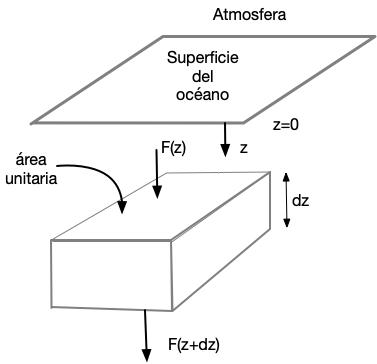
\includegraphics[width=0.50\textwidth]{COS_model.png}
\caption{Diagrama del ejercicio}
}
\label{COS_fig}
\end{figure}
\begin{ejemplo} {continuacion}

Como el volumen de la losa es $1\cdot \mathrm{d}z$ 
\begin{equation}
\textrm{el flujo neto de COS en una unidad de volumen de la losa} =-\frac{\mathrm{d}F(z)}{\mathrm{d}z}
\label{flux_COS}
\end{equation}
Si $D$ coeficiente de difusi\'on en remolino,
\begin{equation}
F(z)=-D\frac{\mathrm{d}C(z)}{\mathrm{d}z}
\label{dif_COS}
\end{equation}
donde $C(z)$ es la concentraci\'on de COS a la distancia $z$ debajo de la superficie del oc\'eano, y el signo negativo surge porque la difusi\'on ocurre en la direcci\'on opuesta a la del aumento de la concentraci\'on. En el presente caso, la concentraci\'on de COS es mayor en la superficie del oc\'eano y disminuye hacia abajo; por lo tanto, el flujo de COS es descendente en el oc\'eano. De las ecuaciones. (\ref{flux_COS}) y (\ref{dif_COS})
\begin{equation}
\textrm{el flujo neto de COS en una unidad de volumen de la losa} =D\frac{\mathrm{d}^2C(z)}{\mathrm{d}z^2}
\label{flux2_COS}
\end{equation}
\noindent Si $k$ es el coeficiente de tasa de primer orden para la destrucci\'on qu\'{\i}mica de COS en aguas marinas 

\begin{equation}
\textrm{tasa de destrucci\'on de COS en una unidad de volumen de la losa} =kC(z)
\label{des_COS}
\end{equation}
\noindent En condiciones de estado estacionario, de las ecuaciones (\ref{flux2_COS}) y  (\ref{des_COS})
\begin{equation}
\frac{\mathrm{d}C(z)}{\mathrm{d}t}=D\frac{\mathrm{d}^2C(z)}{\mathrm{d}z^2}-kC(z)=0
\label{cc_COS}
\end{equation}
La soluci\'on de la ecuaci\'on~\ref{cc_COS} es
\begin{equation}
C(z)=C(0)\exp(-z/H)
\label{c_cos}
\end{equation}
\noindent donde H (una altura de escala) est\'a dada por
\begin{equation}
H=\left( \frac{D}{k}\right)^{1/2} =  \left( \frac{0.0050}{5.0\times10^{-6}}\right)=\SI{32}{\metre}
\label{H_COS}
\end{equation}

Ahora se pueden responder las tres preguntas:

\begin{enumerate}
\item Cuando $C(z)=C(0)/2$, tenemos de las ecuaciones (\ref{c_cos}) y  (\ref{H_COS}) 
\begin{equation*}
\frac{1}{2}=\exp\left(-\frac{z}{H} \right)=\exp\left( -\frac{z}{32}\right)
\end{equation*}
Por lo tanto, z = 22m
\item La densidad de la columna de COS en el oc\'eano es la masa total de COS en una columna de unidad de \'area de secci\'on transversal que se extiende desde la superficie hasta el fondo del oc\'eano. Por lo tanto

\begin{eqnarray*}
\textrm{Densidad de columna de COS} &=& \int_{z=0}^\infty C(z)\,\mathrm{d}z \\
       &=&  \int_{z=0}^\infty C(0)\exp\left(-\frac{z}{H}\right)\,\mathrm{d}z  \\
       &=& C(0)H \\
       &=& (1.0\times10^{-11})\times 32 \\
       &=& 3.2\times10^{-10}\si{\kilo\gram\per\square\metre}
\end{eqnarray*}
%
\item De la ecuaci\'on de tiempo de vida de un compuesto $\tau=M/F$
donde $M$ es la cantidad de sustancia qu\'{\i}mica en, digamos, la columna de secci\'on transversal unitaria que consideramos anteriormente y $F$ es la salida (tasa de eliminaci\'on m\'as tasa de destrucci\'on) de la sustancia qu\'{\i}mica de la columna. Por lo tanto, la vida media de una mol\'ecula de COS en el oc\'eano viene dada por:
\begin{eqnarray*}
\tau & = & \frac{C(0)H}{k\int_0^\infty C(z)\,\mathrm{d}z } \\
& =& \frac{C(0)H}{kC(0)H}  \\ 
& =& \frac{1}{k}  \\ 
&=& \frac{1}{5.0\times10^{-6} \si{\second}^{-1}}\\
&=& 2.3\, \textrm{d\'{\i}as} 
\end{eqnarray*}
\end{enumerate}
\end{ejemplo}
\subsection{Tierra s\'olida}\index{fuentes!tierra@tierra s\'olida}
Los volcanes son la fuente geoqu\'{\i}mica m\'as importante de gases traza en al atm\'osfera. Aunque son muy localizados y muy variables, cuando las emisiones volc\'anicas son lanzadas a la estratosfera (o superior), pueden dispersarse r\'apidamente por todo el mundo y tener largos tiempos de residencia (1 a 2 a\~no). El polvo fino  llega a dar varias vueltas alrededor de la Tierra. Los aerosoles producidos a partir de los gases pueden permanecer en la estratosfera durante varios a\~nos. Esto, a su vez, da lugar a un enfriamiento medio global en la superficie de $\sim$ \SI{0.4}{\celsius} en el a\~no siguiente a la erupci\'on; este enfriamiento llega a desaparecer despu\'es de $\sim$3 a\~nos a medida que disminuye el polvo en la atm\'osfera. Adem\'as de cenizas y part\'{\i}culas de polvo, los volcanes emiten \ce{H2O}, \ce{CO2}, \ce{SO2}, \ce{H2S}, COS, \ce{CS2}, HCl, HF, HBr, \ce{CH4}, \ce{CH3Cl}, \ce{H2}, CO y varios metales pesados vol\'atiles (p. ej., Hg). Las rocas son una fuente de  cantidades peque\~nas de ciertos gases y son las principales fuentes de los gases He, Ar y Rn en la atm\'osfera. El helio se produce principalmente del decaimiento radiactivo del uranio-238 y torio-232- No se acumula en la atm\'osfera debido a que es tan ligero que escapa de la exosfera\index{exosfera}. El arg\'on se ha acumulado durante eones debido a la desintegraci\'on radiactiva del potasio-40 de rocas.

Las rocas carbonatadas, como la piedra caliza, que se presenta principalmente como calcita (es decir, \ce{CaCO3}), contienen 100,000 veces m\'as carbono que la atm\'osfera, pero la mayor parte est\'a secuestrada. Sin embargo, las rocas carbonatadas y los sedimentos marinos participan en un ciclo de per\'{\i}odo largo con el \ce{CO2} atmosf\'erico como se muestra a continuaci\'on. La erosi\'on de la calcita por el \ce{CO2} disuelto en la lluvia y en aguas dulces (r\'{\i}os y lagos) se puede representar por

\begin{footnotesize}
\begin{eqnarray}
\ce{CO2}(g) + \ce{H2O} &\rightleftarrows& \ce{CO2}(ac) + \ce{H2O}(l)  \label{eq_co2h2o}\\
\ce{2H2O}(l) +   \ce{CO2}(ac)&\rightleftarrows&   \ce{H3O^+}(ac) +  \ce{HCO3^-}(ac) \label{eq_co2}\\
\ce{CaCO3}(s) +   \ce{H3O^+}(ac) +  \ce{HCO3^-}(ac) &\rightleftarrows& \ce{Ca^{2+}}(ac) + \ce{2HCO3^-}(aq) + \ce{H2O}(l)\label{eq_caco3}\\\hline
\textrm{Neto:       }   \ce{CaCO3}(s) +\ce{CO2}(g) + \ce{H2O}(l)  &\rightleftarrows&\ce{Ca^{2+}}(ac) + \ce{2HCO3^-}(aq)  \label{eq_cca}
\end{eqnarray}
\end{footnotesize}

La reacci\'on (\ref{eq_co2h2o}) representa el equilibrio entre el \ce{CO2} en el aire y en los r\'{\i}os y lagos de agua dulce. En la reacci\'on (\ref{eq_co2}), el \ce{CO2} recibe un \ce{OH^-}  del \ce{H2O} para formar el \'acido muy d\'ebil (es decir, poco ionizado) \ce{HCO3^-} (el ion bicarbonato), y en la reacci\'on (\ref{eq_caco3}) el \ce{H3O+} remueve \ce{CO3^{2-}} del \ce{CaCO3} para formar otro ion bicarbonato\index{bicarbonato}. La reacci\'on directa de (\ref{eq_caco3}) representa la erosi\'on de la calcita por el \ce{CO2}  disuelto en aguas dulces.

Los productos de la \gls{meteorizacion} ,en el lado derecho de la reacci\'on~\ref{eq_cca}, eventualmente ingresan a los oc\'eanos, donde se precipitan para formar nuevos sedimentos (lo contrario de la reacci\'on (\ref{eq_cca})). A trav\'es del levantamiento de las regiones de la plataforma continental, la subducci\'on de sedimentos marinos hacia el manto superior y la corteza inferior de la Tierra y las erupciones volc\'anicas, estos productos eventualmente regresan a los sedimentos continentales, completando as\'{\i} este ciclo geoqu\'{\i}mico. Los tiempos de residencia del \ce{Ca^{2+}}(aq) y del \ce{HCO3^-}(aq) en los oc\'eanos son $\sim 8\times 10^5$ y $\sim7.5 \times 10^4$ a\~nos, respectivamente.

\begin{ejemplo}{Disoluci\'on de \ce{CO2} en agua} 
Cuando el \ce{CO2} se disuelve en agua pura \textquestiondown qu\'e reacciones se producen?

\textbf{Respuesta:}

\begin{footnotesize}
\begin{eqnarray}
\ce{CO2}(g) + \ce{H2O} &\rightleftarrows& \ce{H2CO3}(ac) \\
\ce{H2CO3}(ac) + \ce{H2O}(l) &\rightleftarrows&  \ce{HCO3^-}(ac) + \ce{H3O^+}(ac) \\
 \ce{HCO3^-}(ac) + \ce{H2O}(l) &\rightleftarrows&  \ce{CO3^{-2}}(ac) + \ce{H3O^+}(ac) \\ \hline
 \textrm{Neto:         } \ce{CO2}(g) + 3\ce{H2O} &\rightleftarrows& \ce{CO3^{-2}}(ac) +2 \ce{H3O^+}(ac) 
 \end{eqnarray}
\end{footnotesize}
\end{ejemplo}

\subsection{Oc\'eanos}\index{fuentes!oceano@oc\'eano}
La mayor\'{\i}a de los gases que pasan de los oc\'eanos al aire se originan en procesos biol\'ogicos, que se analizan en la subsecci\'on (\ref{subbio}). Adem\'as, como vimos en la subsecci\'on anterior, los oc\'eanos pueden participar en el ciclo de gases entre la Tierra s\'olida y la atm\'osfera. 

Los oc\'eanos son un enorme reservorio de aquellos gases que son apreciablemente solubles en agua. Los oc\'eanos pueden servir como fuente y sumidero de gases traza en la atm\'osfera.

\subsection{Formaci\'on in situ en la atm\'osfera.}\index{atmosfera@atm\'osfera!fuentes de contaminantes}

Las reacciones qu\'{\i}micas en la atm\'osfera son una fuente importante y un sumidero de muchos constituyentes traza. Los gases traza emitidos por la biosfera, la Tierra s\'olida y los oc\'eanos generalmente se encuentran en un estado de oxidaci\'on reducido (es decir, m\'as bajo) (por ejemplo, C, N y S), pero cuando regresan a la superficie de la Tierra generalmente se encuentran en un estado de  mayor oxidaci\'on.

Los procesos que producen estas transformaciones se pueden dividir en reacciones de fase gaseosa homog\'enea, fase acuosa homog\'enea y reacciones heterog\'eneas.

 \section{El esmog}\index{esmog}
\label{sgmog}

 La contaminaci\'on ambiental se encuentra presente en nuestra vida y es producto de las actividades de la vida cotidiana tanto en las ciudades como en el campo. La principal causa de la contaminaci\'on en el aire es debido a la combusti\'on, y \'esta es de suma importancia para el ser humano. Cuando ocurre la combusti\'on perfecta o te\'orica, el carbono e hidr\'ogeno del combustible se combinan con el ox\'{\i}geno del aire desprendiendo calor, luz y generando bi\'oxido de carbono y vapor de agua. Sin embargo las impurezas del combustible, el mezclado imperfecto, la temperatura exterior afectan la combusti\'on gener\'andose impurezas tales como mon\'oxido de carbono, di\'oxido de azufre, \'oxidos de nitr\'ogeno, holl\'{\i}n y combustible no quemado ---todos ellos son contaminantes del aire.
 
 El esmog es la combinaci\'on de part\'{\i}culas de humo de fuentes industriales con neblina produciendo un color negro-amarillento cerca de la superficie (nieblumo)\index{esmog!nieblumo}. La combusti\'on de gasolina puede crear otro problema de contaminaci\'on conocido como ``esmog fotoqu\'{\i}mico''. Este se genera cuando los contaminantes primarios (\'oxidos de nitr\'ogeno y COV) interact\'uan bajo la influencia de la luz solar para producir una mezcla de cientos de sustancias t\'oxicas diferentes conocidas como contaminantes secundarios. Es una bruma marr\'on que contamina las ciudades. Puede hacer dif\'{\i}cil el respirar para algunas personas y reduce la visibilidad.

 \subsection{Europa}
En diciembre de 1930, una regi\'on altamente industrializada del Valle de Meuse, en B\'elgica, se cubri\'o durante 3 d\'{\i}as de una espesa niebla, por lo que cientos de personas enfermaron y 60 murieron ---m\'as de 10 veces el n\'umero normal.  

En Inglaterra durante 9 d\'{\i}as, en enero de 1931, murieron 592 personas --lo que nuevamente representaba un considerable incremento en la tasa de mortalidad. En 1948, en Donora, Pennsylvania, un peque\~no pueblo en donde hab\'{\i}a plantas qu\'{\i}micas y acerer\'{\i}as se cubri\'o por una niebla durante 4 d\'{\i}as,  enferm\'o casi la mitad de sus 14,000 habitantes. Murieron 20 personas. No fue hasta que una gran capa de niebla cubri\'o Londres en 1952 cuando se hizo totalmente evidente el siniestro potencial de la contaminaci\'on del aire. La niebla dur\'o desde el 5 de diciembre hasta el 8, y 10 d\'{\i}as despu\'es se supo que el n\'umero total de muertes en la regi\'on principal de Londres sobrepasaba en 4,000 al promedio. Las estad\'{\i}sticas indicaron que casi todos los que hab\'{\i}an muerto inesperadamente ten\'{\i}an antecedentes cl\'{\i}nicos de bronquitis, enfisema o trastornos card\'{\i}acos, y que las personas clasificadas en la \'ultima categor\'{\i}a, eran las m\'as vulnerables. Nuevamente, en enero de 1956, se produjeron 1,000 muertes m\'as debido a una extensa niebla.

 
 \subsection{Los Angeles}
En contraste con la contaminaci\'on en Londres los episodios de contaminaci\'on en Los Angeles y la Ciudad de M\'exico se dan en situaciones de cielos despejados con sistemas de alta presi\'on que limitan la dispersi\'on de contaminantes. En este caso las emisiones primarias de los procesos industriales, comerciales y del transporte reaccionan en la atm\'osfera generando nuevos contaminantes que afectan la salud de los seres humanos, animales, plantas  y afectando a los materiales.

\subsection{Clasificaci\'on de Contaminantes}

Los contaminantes atmosf\'ericos se pueden clasificar de diversas maneras, una de ellas es por su composici\'on:\index{contaminante!clasificaci\'on}

\begin{itemize}
\item \textbf{Org\'anicos} Contienen carbono, hidr\'ogeno (\ce{CH4}) y pueden incluir ox\'{\i}geno (HCHO), nitr\'ogeno (\ce{CH3NH2}), azufre (DMS).
\item \textbf{Inorg\'anicos} Compuestos de azufre (\ce{SO2}, \ce{H2S}), nitr\'ogeno (\ce{NO_$x$}), halogenados (CFC)\index{CFC}, metales pesados (As, Pb, Cd, etc)
\end{itemize}
Por su estado f\'{\i}sico:
\begin{itemize}
\item Gases y vapores
\item Part\'{\i}culas (s\'olidas y l\'{\i}quidas).
\end{itemize}

A su vez las part\'{\i}culas se pueden clasificar de acuerdo a con su tama\~no, como se muestra en el \textbf{Cuadro~\ref{part:1}} en p\'agina~\pageref{part:1}

Tambi\'en se puede categorizar los contaminantes por su origen de la siguiente  forma:\index{contaminante!primarios}\index{contaminante!secundario}
\begin{description}
\item[Primarios] Aquellos que son emitidos directamente
dentro de la atm\'osfera. Como lo son el mon\'oxido de nitr\'ogeno (NO), di\'oxido de azufre (\ce{ SO2}), el mon\'oxido de carbono (CO).
\item[Secundarios] Creados a trav\'es de reacciones y procesos en la
atm\'osfera. Como el ozono (\ce{O3}), tri\'oxido de azufre (\ce{SO3}) y el nitrato de
peroxiacilo (PAN)\index{PAN}.
\end{description}
\section{Contaminantes criterio}\index{contaminante!criterio}
\label{ccriterio}

De todos los contaminantes posibles existe un conjunto de ellos que se emplean para calificar la calidad del aire  y se les conoce como  \textit{contaminantes criterio}, los contaminantes criterio son seleccionados debido a que pueden provocar efectos a la salud y son los que se muestran en el  \textbf{Cuadro~\ref{contcrit}}.
\begin{table}[htb]
\caption{Contaminantes Criterio}
\label{contcrit}
\begin{center}
\begin{tabular}{ll}\hline
Mon\'oxido de carbono & CO\\
Di\'oxido de azufre & \ce{SO2}\\
\'oxidos de nitr\'ogeno &NO$_x$\\
Ozono & \ce{O3}\\
Part\'{\i}culas & \gls{PST}/\ce{PM10},\ce{PM_{2.5}}\\
Plomo& Pb\\ \hline
\end{tabular}
\end{center}
\end{table}

De todos los compuestos que se han presentado los hidrocarburos (COV)\index{COV} no son contaminantes criterio, pero se estudian muy de cerca por su rol en la producci\'on de ozono:

\begin{center}
COVs $+$ NO$_x +$luz solar $\longrightarrow$ esmog fotoqu\'{\i}mico (\ce{O3}) 
\end{center}

\subsection{Mon\'oxido de carbono (CO)}
\index{CO}
Es gaseoso, inodoro e incoloro es resultado de la combusti\'on incompleta de los veh\'{\i}culos, el 70\% del CO proviene de los veh\'{\i}culos y presenta un perfil diurno, con concentraciones m\'aximas en horas pico de tr\'ansito.

\subsubsection{Efectos a la salud:}
\index{CO}
El CO se puede ligar a la sangre en lugar del di\'oxido de carbono (\ce{CO2}) por lo que puede ser asfixiante al reducir el ox\'{\i}geno (\ce{O2}) transportado -- disminuye la actividad cerebral, incrementa la frecuencia card\'{\i}aca. Los efectos dependen del nivel de actividad.
\begin{equation}
\%\ce{COHb}  = 0.005[\ce{CO]}^{0.85}(\alpha t)^{0.63}
\end{equation}
Donde:

\begin{tabular}{r @{---}l}
$\%\gls{COHb} $ & Carboxihemoglobina en la sangre en por ciento de sa\-tu\-ra\-ci\'on.\\
$[\ce{CO}]$ &Concentraci\'on de CO en ppm\\
$\alpha$ & Coeficiente de actividad ( 0.94 sedentario, 3 trabajo pesado)\\
$t$ & tiempo de exposici\'on en minutos\\
\end{tabular}

Algunos efectos por la cantidad de CO en la sangre son los siguientes:
\begin{itemize}
\item 2.5\% se muestran algunos efectos ligeros.
\item 5\% Se notan efectos psicomotores.
\item 10\% Mareos y dolor de cabeza.
\item 50\% Mortal.
\end{itemize}

\subsubsection{Fuentes de exposici\'on:}
Intersecciones muy transitadas, vivir cerca de vialidades transitadas, fumar.
Se requieren de 3 a 4 horas para alcanzar niveles altos de concentraci\'on de COHb, y
se requieren de 3 a 4 horas para recobrarse de la exposici\'on.

\subsection{Compuestos de azufre}\index{azufre!compuestos}
Este contaminante puede producir, incluso a grandes distancias de la fuente de emisi\'on, efectos adversos sobre la salud (tales como irritaci\'on e inflamaci\'on del sistema respiratorio, afecciones e insuficiencias pulmonares, alteraci\'on del metabolismo de las prote\'{\i}nas, dolor de cabeza o ansiedad), sobre la biodiversidad, los suelos y los ecosistemas acu\'aticos y forestales (puede ocasionar da\~nos a la vegetaci\'on, degradaci\'on de la clorofila, reducci\'on de la fotos\'{\i}ntesis y la consiguiente p\'erdida de especies) e incluso sobre las edificaciones, a trav\'es de procesos de acidificaci\'on, pues una vez emitido, reacciona con el vapor de agua y con otros elementos presentes en la atm\'osfera, de modo que su oxidaci\'on en el aire da lugar a la formaci\'on de \'acido sulf\'urico.

Adem\'as, tambi\'en act\'ua como precursor de la formaci\'on de sulfato am\'onico, lo que incrementa los niveles de \ce{PM10} y \ce{PM_{2.5}}, con graves consecuencias igualmente sobre la salud.

\subsubsection{Fuentes de emisi\'on del di\'oxido de azufre} Las principales fuentes de azufre en la atm\'osfera son el uso de combustibles f\'osiles y las exhalaciones volc\'anicas\index{volcan@volc\'an}. El compuesto que principalmente se emite es el di\'oxido de azufre (\ce{SO2}). La fuente  \gls{antropica} principal es la quema de combustibles conteniendo azufre, el 85\% del total de emisiones proviene de esta fuente. Algunas industrias de la fundici\'on, la refinaci\'on, la minera --  tienen normas de emisi\'on de este compuesto.

El contenido de azufre en los combustibles abarca el intervalo de 0.05 a 6\% en los combustibles l\'{\i}quidos y en el carb\'on. Cuando se queman se emite el di\'oxido de azufre (\ce{SO2}).
Produce lluvia \'acida\index{lluiva@lluvia \'acida}, tambi\'en se condensa en part\'{\i}culas formando \ce{SO_4^=} durante el per\'{\i}odo de d\'{\i}as
\begin{itemize}
\item Exposici\'on a 1 ppm de \ce{SO2} por 15--20 min se observan cambios en el pulso y
respiraci\'on.
\item 0.3 ppm por 1--3 d\'{\i}as enfermedades cardio-respiratorias, muertes en Londres.\index{Londres}
\item 0.002 ppm por un a\~no, incrementa las admisiones al hospital.
\end{itemize}

\subsection{Compuestos de nitr\'ogeno}
\index{nitrogeno@nitr\'ogeno!compuestos de} 
En la atm\'osfera se encuentran diversas formas del nitr\'ogeno, tanto oxidadas como reducidas:

\textbf{Formas oxidadas:}
\begin{itemize}
\item NOx= NO + \ce{NO2},
\item NOy =NOx + \ce{NO3} + HONO + \ce{HNO3} + \ce{N2O5} + PAN
\item NOz = NOy -NOx
\end{itemize}

\textbf{Formas reducidas:}
\begin{itemize}
\item  Amon\'{\i}aco\index{amoniaco@amon\'{\i}aco} (\ce{NH3})
\item Cianuro de hidr\'ogeno (HCN)\index{cianuro} 
\item Aminas:
\begin{itemize}
\item Alif\'aticas\index{aminas!alifaticas@alif\'aticas}: \ce{RNH2} 
\item Arom\'aticas\index{aminas!aromaticas@arom\'aticas}  RR'NH y RR'R''N 
\end{itemize}
\item N\'{\i}tratos: RCN
\end{itemize}
 donde R, R' R'' = son grupos alquilos\index{grupo!alquilo}  o \gls{arilo}\index{grupo!arilo} .

\subsubsection{\'oxidos de Nitr\'ogeno (NO$_x$)}
La suma de \ce{NO} + \ce{NO2} se refiere como NO$_x$, principalmente proviene de la combusti\'on:
\begin{description}
\item[NO$_x$ Termal] Cuando el \ce{N2}  y el \ce{O2} se calientan a altas temperaturas
($>400^\circ C$)
\item[NO$_x$ Combustible] Del nitr\'ogeno contenido en el combustible.
\end{description}
La emisiones de NO$_x$ son principalmente NO, \'este reacciona y forma el \ce{NO2} que absorbe la luz.
%\begin{eqnarray}
%\ce{NO2} + \textrm{hidrocarburos}&\longrightarrow&\textrm{esmog}\index{esmog}\\
%\ce{NO2}+ \ce{OH}\cdot &\longrightarrow&\ce{HNO3} \: \textrm{(Lluvia \'acida)} \index{lluiva@lluvia \'acida}
%\end{eqnarray} 

\subsubsection{Control} En emisiones de fuentes estacionarias y en motores de veh\'{\i}culos. Reduciendo la temperatura de combusti\'on y con combustibles con bajo nitr\'ogeno (N). Altas temperaturas disminuyen el mon\'oxido de carbono (CO) pero incrementan la emisi\'on de  NO$_x$.

\subsection{Ozono (O$_3$)}\label{o3_salud}\index{ozono}
El ozono no se emite directamente a la atm\'osfera, se produce mediante una serie de reacciones que involucran a los \'oxidos de nitr\'ogeno, hidrocarburos y la luz solar ($h\nu$). El ozono posee dos efectos -- da\~nos a la salud y a los materiales.

Efectos del ozono en materiales:
\begin{itemize}
\item Reduce la vida \'util de llantas y hules.
\item Puede da\~nar a la vegetaci\'on (reduce la producci\'on agr\'{\i}cola)
\end{itemize}
Efectos del ozono en la salud:
\begin{itemize}
\item Irritaci\'on de ojos.
\item Constricci\'on del pecho, irritaci\'on en la garganta.
\item Altas concentraciones agravan las enfermedades respiratorias.
\end{itemize}
La  formaci\'on de ozono depende de la disponibilidad del \ce{NO2}  y la destrucci\'on depende de la concentraci\'on del NO. Sin embargo en las ciudades el efecto global de las reacciones con hidrocarburos (COV) es convertir el \ce{NO} a \ce{NO2} por lo cual hace que se incremente la concentraci\'on del \ce{O3}.

\begin{table}[hbt]
\caption{Ozono en la atm\'osfera}
\label{ozon:1}
\begin{center}
{\footnotesize \begin{tabularx}{.9\textwidth}{X|X}
\textbf{Ozono Troposf\'erico}&\textbf{Ozono Estratosf\'erico}\\ \hline \hline
Localizado entre $0$--$10$ \si{\kilo\metre}& Localizado entre $15$--$35$ \si{\kilo\metre}\\
Contiene el $10$\% del ozono de la atm\'osfera&
Contiene el $90$\% del ozono de la atm\'osfera\\
Impacto da\~nino: efectos t\'oxicos en seres humanos y vegetaci\'on&
Rol ben\'efico: Act\'ua como escudo a la radiaci\'on UV\\
T\'opicos actuales: -- Episodios de alta concentraci\'on en superficie en ciudades.&
T\'opicos actuales: Disminuci\'on en la concentraci\'on. Hoyo de ozono en la
primavera ant\'artica\\\hline
\end{tabularx}}
\end{center}
\end{table}

El control del ozono se da a trav\'es de controlar sus precursores, \'oxidos de nitr\'ogeno, y compuesto org\'anicos. Si el aire se encuentra ``atrapado'' por la
orograf\'{\i}a y condiciones meteorol\'ogicas como la inversi\'on t\'ermica, esto puede empeorar el problema como en  Los Angeles, la Ciudad de M\'exico, Grecia y en el Valle Fraser (frontera EE-Canad\'a).

\paragraph{Nota sobre ozono}
\index{ozono!troposf\'erico}
\index{ozono!estratosf\'erico}
Existen dos diferentes zonas donde se encuentra el ozono, el troposf\'erico (nivel del suelo) y el estratosf\'erico. En el \textbf{Cuadro~\ref{ozon:1}} se pueden observar las
caracter\'{\i}sticas y efectos que posee el ozono en las diferentes zonas.



\subsection{Part\'{\i}culas}
Se definen como part\'{\i}culas a cualquier material disperso (s\'olido o l\'{\i}quido) cuyos componentes individuales tienen un tama\~no mayor que una mol\'e\-cula pero menor a \SI{500}{\micro\metre}.  En el \textbf{Cuadro \ref{part:1}}  se enlistan en diferentes categor\'{\i}as las part\'{\i}culas:

\begin{table}[h!]
\caption{Definici\'on de las part\'{\i}culas suspendidas en el aire}
\label{part:1}
\begin{center}
{\footnotesize \begin{tabularx}{\linewidth}{>{\setlength{\hsize}{.35\hsize}}X%
>{\setlength{\hsize}{1.65\hsize}}X} \hline
{\footnotesize Part\'{\i}culas} & Cualquier material, excepto agua no combinada, que
existe en estado s\'olido o l\'{\i}quido en la atm\'osfera o en una corriente de gas
en condiciones normales.\\
{\footnotesize Aerosol} & Una dispersi\'on de part\'{\i}culas microsc\'opicas, s\'olidas o
l\'{\i}quidas. \\
{\footnotesize  Polvo} & Part\'{\i}culas s\'olidas de un tama\~no mayor que el coloidal, capaces
 de estar en suspensi\'on temporal en el aire.\\
{\footnotesize Ceniza fin}a& Part\'{\i}culas de ceniza finamente divididas arrastradas
por el gas de combusti\'on. Las part\'{\i}culas pueden contener combustible no
quemado\\ 
{\footnotesize  Niebla} &Aerosol visible.\\
{\footnotesize Vapores}& Part\'{\i}culas formadas por la condensaci\'on, sublimaci\'on,
o reacci\'on qu\'{\i}mica, predominantemente mayores de \SI{1}{\micro\metre} (humo de
tabaco).\\
{\footnotesize Neblina} & Dispersi\'on de peque\~nas gotas de l\'{\i}quido de suficiente tama\~no como
para caer.\\
 {\footnotesize Part\'{\i}cula}& Masa discreta de materia s\'olida o l\'{\i}quida.\\
{\footnotesize Humo}& Part\'{\i}culas peque\~nas arrastradas por los gases, que resultan
dela combusti\'on.\\
{\footnotesize Holl\'{\i}n}& Una aglomeraci\'on de part\'{\i}culas de carb\'on.\\ \hline
\end{tabularx}}
\end{center}
\end{table}
\subsubsection{Efectos en la salud} 
Las part\'{\i}culas menores a \SI{10}{\micro\metre} (PM$_{10}$) y \SI{2.5}{\micro\metre}  (PM$_{2.5}$) constituyen el principal riesgo para la salud humana. Al ser inhaladas, penetran en el tracto respiratorio: las PM$_{10}$ se depositan en v\'{\i}as superiores, mientras las PM$_{2.5}$ alcanzan los alv\'eolos pulmonares. Esto desencadena procesos inflamatorios sist\'emicos, reducci\'on de la capacidad pulmonar (2-3\% por cada \SI{10}{\micro\gram\per\cubic\metre}  de PM$_{2.5}$) y exacerbaci\'on de enfermedades cardiovasculares. La exposici\'on cr\'onica se relaciona con:
\begin{itemize}
    \item Incremento del 12\% en mortalidad por c\'ancer de pulm\'on (por cada \SI{10}{\micro\gram\per\cubic\metre} anual de PM$_{2.5}$) \index{mortalidad!particulas@part\'{\i}culas}
    \item Desarrollo de EPOC\footnote{Enfermedad pulmonar obstructiva cr\'onica} en poblaciones urbanas (OR = 1.29; IC95\%: 1.04–1.59)\index{EPOC}
    \item Neurotoxicidad en ni\~nos (p\'erdida de 1-2 puntos de CI por cada \SI{5}{\micro\gram\per\cubic\metre} de PM$_{2.5}$)
\end{itemize}

\paragraph{Nota sobre las part\'{\i}culas}
Cuando se especific\'o la norma de part\'{\i}culas, \'estas se regular\'on como Part\'{\i}culas Suspendidas Totales (PST)\index{PST}. Esta fue la medida de concentraci\'on de part\'{\i}culas en el aire.\index{particulas@part\'{\i}culas}

En 1987 en EU la norma cambi\'o a PM$_{10}$ -- toda part\'{\i}cula menor a  \SI{10}{\micro\metre} en di\'ametro y en 1997, otra norma de part\'{\i}culas se adicion\'o --- \ce{PM_{2.5}} -- toda part\'{\i}cula menor a \SI{2.5}{\micro\metre}  en di\'ametro.

\subsection{Plomo (Pb)}
\index{plomo}
Hasta 1980, la principal fuente de emisiones de plomo atmosf\'erico proven\'{\i}a de los veh\'{\i}culos que utilizaban \textbf{gasolina con tetraetilo de plomo} (\ce{(C2H5)4Pb}), un aditivo antidetonante. \index{antidetonante}Este compuesto se a\~nad\'{\i}a en concentraciones de \textbf{1.1 gramos por gal\'on} (\SI{ 0.29}{\gram\per\litre}), equivalente al 61\% en peso del aditivo completo \textit{TEL} (Tetraethyl Lead). \index{tetraetilo de plomo}

\subsubsection{Efectos en la salud} El plomo representa un riesgo toxicol\'{o}gico significativo, particularmente en poblaciones infantiles. Sus principales v\'{\i}as de exposici\'{o}n incluyen:

\begin{itemize}
    \item \textbf{Inhalaci\'{o}n}: 
    \begin{itemize}
        \item Emitido como sales de plomo (ej. \ce{PbSO4}) depositadas cerca de v\'{\i}as de tr\'{a}nsito
        \item Part\'{\i}culas transportadas a interiores por calzado (tama\~no $\sim$ \SIrange{2}{10}{\micro\metre})
        \item Resuspensi\'{o}n atmosf\'{e}rica en espacios cerrados (factor $3--5\times$ mayor que exterior)
    \end{itemize}
    
    \item \textbf{Ingesti\'{o}n}:
    \begin{itemize}
        \item Contaminaci\'{o}n h\'{\i}drica por tuber\'{\i}as de plomo (pH $<$ 7 aumenta lixiviaci\'{o}n)
        \item Pinturas con base de plomo (comunes en construcciones anteriores a 1980)
        \item Suelos contaminados (bioaccesibilidad $\sim$ 25-60\%)
    \end{itemize}
\end{itemize}

\textbf{Mecanismo de toxicidad}:
\begin{itemize}
    \item Sustituci\'{o}n del hierro en rutas metab\'{o}licas (afinidad por grupos sulfhidrilo)
    \item Neurotoxicidad aguda en ni\~nos (DL$_{50}$ = \SIrange{100}{150}{\micro\gram\per\deci\liter}):
    \begin{itemize}
        \item Reducci\'{o}n de coeficiente intelectual (2-5 puntos por \SI{10}{\micro\gram\per\deci\liter})
        \item Da\~no cerebral irreversible (mielinizaci\'{o}n alterada)
        \item Trastornos conductuales (TDAH\footnote{Trastorno de deficit de atenci\'on e hiperactividad.}, agresividad)
    \end{itemize}
    
    \item Umbrales cr\'{\i}ticos (CDC 2023):
    \begin{itemize}
        \item \SI{20}{\micro\gram\per\deci\liter}: Da\~nos hematol\'{o}gicos (anemia hemol\'{\i}tica)
        \item \SI{50}{\micro\gram\per\deci\liter}: Encefalopat\'{\i}a aguda (mortalidad $\sim$ 5-10\%)
    \end{itemize}
\end{itemize}

\subsection{Visibilidad y la calidad del aire}\index{visibilidad!calidad del aire}

La dispersi\'on de la radiaci\'on electromagn\'etica en la atm\'osfera est\'a gobernada por el par\'ametro de tama\~no $\alpha = \frac{2\pi r}{\lambda}$, donde $r$ es el radio de la part\'{\i}cula y $\lambda$ la longitud de onda. Cuando $\alpha \approx 1$ (dispersi\'on de Mie), se produce la m\'axima eficiencia de dispersi\'on. Para la luz visible ($\lambda = \SIrange{0.38}{0.70}{\micro\metre}$), esto corresponde a part\'{\i}culas con di\'ametros d = \SIrange{0.12}{0.22}{\micro\metre}.
\subsubsection{Par\'ametros operacionales}\index{visibilidad!horizontal}
\begin{itemize}
    \item \textbf{Visibilidad horizontal} (f\'ormula de Koschmieder\index{Koschmieder}):\label{fKoschmieder}
    \begin{equation}
    V = \frac{3.912}{\beta_{ext}} \quad [\si{\kilo\metre}], \quad \beta_{ext} = \sum N_i\sigma_{ext,i}
    \end{equation}
    
    \item \textbf{Umbrales significativos}:
    \begin{itemize}
        \item $2,000$ part/cm$^3$: Obscurecimiento de relieves monta\~nosos
        \item $100,000$ part/cm$^3$: $V \approx \SI{1.6}{\kilo\metre}$ (1 milla).
        \item $8-10$ ppm de \ce{NO2}: $V \leq \SI{1.6}{\kilo\metre}$.
    \end{itemize}
    
    \item \textbf{Efecto de humedad}:
    \begin{itemize}
        \item HR > 70\%: Crecimiento higrosc\'opico ($\times 1.5-4$ en $d$)
        \item Aumento equivalente en $\beta_{ext}$ de 2--5 veces
    \end{itemize}
\end{itemize}

\subsubsection{Contexto regulatorio}\footnote{
Evoluci\'on de normas de part\'{\i}culas:
\begin{itemize}
    \item PST (Part\'{\i}culas Suspendidas Totales): Medida hist\'orica.
    \item PM$_{10}$ (1987 EU): Part\'{\i}culas < \SI{10}{\micro\metre} .
    \item PM$_{2.5}$ (1997 EU): Part\'{\i}culas < \SI{2.5}{\micro\metre}.
\end{itemize}
}

Los principales gases que influyen en la visibilidad son \ce{SO2}, \ce{NO}, y \ce{H2O}, donde:
\begin{itemize}
    \item \ce{SO2}: Contribuye a formaci\'on de aerosoles sulfatados
    \item \ce{NO}: Precursor de \ce{NO2} y nitratos
    \item \ce{H2O}: Modula crecimiento de part\'{\i}culas higrosc\'opicas
\end{itemize}

En condiciones pr\'{\i}stinas ($\beta_{ext} < 14\ \text{Mm}^{-1}$) se alcanzan $V > \SI{280}{\kilo\metre}$, mientras que en niebla densa ($\beta_{ext} > 39,000\ \text{Mm}^{-1}$) $V < \SI{0.1}{\kilo\metre}$.

\section{Compuestos t\'oxicos en el aire}
\label{ctox}
\normalsize
El t\'ermino de \emph{compuestos t\'oxicos} se refiere a cualquier sustancia qu\'{\i}mica presente en el aire con potencial de da\~no a la salud o el ambiente. Para prop\'ositos regulatorios, la Agencia de Protecci\'on Ambiental de EE.UU. (EPA) clasifica estos contaminantes en dos categor\'{\i}as:

\begin{itemize}
    \item \textbf{Contaminantes criterio}: 
    \begin{itemize}
        \item Regulados mediante Normas Nacionales de Calidad del Aire (NAAQS) en EEUU y por Normas Oficiales Mexicanas (NOM) en M\'exico
        \item Emitidos en grandes vol\'umenes por m\'ultiples fuentes
        \item Riesgo regional para salud p\'ublica y ecosistemas
        \item Incluyen: 
        \begin{itemize}
            \item Di\'oxido de azufre (\ce{SO2})
            \item Di\'oxido de nitr\'ogeno (\ce{NO2})
            \item Mon\'oxido de carbono (\ce{CO})
            \item Part\'{\i}culas (PM$_{2.5}$/PM$_{10}$)
            \item Ozono troposf\'erico (\ce{O3})
            \item Plomo (\ce{Pb})
        \end{itemize}
    \end{itemize}
    
    \item \textbf{T\'oxicos ambientales}:
    \begin{itemize}
        \item Listado en el \emph{Clean Air Act} (189 compuestos) y en M\'exico es la  \gls{NOM}-165-\gls{SEMARNAT}-2013\footnote{Es el documento regulatorio que establece la lista de sustancias sujetas a reporte para el Registro de Emisiones y Transferencia de Contaminantes (RETC) en M\'exico. Esta norma, publicada el 24 de enero de 2014, tiene como objetivo regular las emisiones y transferencias de contaminantes al aire, agua, suelo y subsuelo, as\'{\i} como en residuos peligrosos y descargas de agua residual.}
        \item Efectos espec\'{\i}ficos: carcinog\'enesis, mutagenicidad, toxicidad reproductiva
        \item Ejemplos detallados en el \textbf{Cuadro~\ref{airtox}}
        \item Metodolog\'{\i}as de an\'alisis de riesgo estandarizadas de \gls{EPA} IRIS y  \gls{CARB} Hot Spots (AB 2588)
    \end{itemize}
\end{itemize}

Los m\'etodos cuantitativos de evaluaci\'on de riesgos aplican a toda sustancia t\'oxica atmosf\'erica, aunque los casos de estudio num\'ericos en este documento se enfocan espec\'{\i}ficamente en los compuestos listados en el \textbf{Cuadro~\ref{airtox}}.

 \begin{table}[!htbp]
\caption{Contaminantes T\'oxicos}
\begin{scriptsize}
\tablefirsthead{  \hline {\bf CAS} & {\bf Compuesto} &{\bf  CAS} &{\bf Compuesto}\\}
\begin{supertabular}{| p{0.10\textwidth}p{0.35\textwidth}p{0.10\textwidth}p{0.35\textwidth} |}\hline%
75070 & Acetaldeh\'{\i}do &133904 & Cloranfen \\
60355 & Acetamina  & 57749 & Clordano\\
75058 & Acetonitrilo & 7782505 & Cloro \\
98862 & Acetofenona & 79118 & Ac. clorac\'etico\\
53963 & 2-Acetilaminofluoreno & 532274 & 2-Cloracetafenona\\
107028 & Acroleina & 108907 & Clorobenceno\\
79061 & Acrilamina & 510156 & Clorobencilato\\
79107 & Ac. acr\'{\i}lico & 67663 & Cloroformo\\
107131 & Acrilonitrilo & 107302 & Clorometil metil eter\\
107051 & Alil cloruro & 126998 & Cloropreno \\
92671 & 4-aminobifenil & 1319773 & Cresoles (isomeros y mezclas)\\
62533 & Anilina &9587 &\emph{o}-Cresol\\
90040 & \emph{o}-Anisidina & 108394 &\emph{m}-Cresol \\
1332214 & Asbestos & 106445 &\emph{p}-Cresol \\
71432 & Benceno (incluyendo& 98828 &Cumeno \\
            & benceno de gasolina) & 94757 &2,4-diclorofenoxiac\'etico,  \\
92875 & Bencidina &  &sales y esteres\\
98077 & Benzotricloro & 3547044 & DDE\\
100447 & Cloruro de Bencilo & 334883 &  Diazometano\\
92524 & Bifenil & 132649 & Dibenzofuranos\\
117817 & Bis(2-etilhexil) ftalato (DEHP) & 96128 & 1,2-Dibromo- 3- cloropropano\\
542881& Bis(clorometil) eter &8742&Dibutilftalato\\
75252 & Bromformo &106467&1,4- Dicloro benceno (p) \\
106990 &1,3-Butadieno &91941& 3,3-Diclorobencidine \\
156627 & Cianamida de calcio &111444&Dicloroetil eter (bis(2-cloroetil)eter)\\
105602& Caprolactama& 542756 &1,3-Dicloropropeno\\ 
133062 & Captan & 62737 & Diclorvos (DDVP)\\
63252 & Carbaril &111422& Dietanolamina\\
75150 & Disulfuro de carbono & 121697 & N,N-Dietilanilina (NN-Dimetilanilina) \\
56235 & Tetracloruro de Carbono &64675&Sulfato de dietilo\\
463581 & Sulfuro de Carbonilo  &110543&Hexano\\
120809 & Catecol & 302012&Hidrazina \\
119904 & 3,3-Dimetoxybencidina &7647010&  \'acido Hidrocl\'orico\\
60117 & Dimetil ainoazoenceno&7664393& Fluoruro de hidr\'ogeno\\
119937 & 1,3-Dimetil bencidine & &(\'acido fluorh\'{\i}drico)\\
79447 & Clouro de Dimetil cabamol&123319&Hidroquinona\\
  68122 & Dimetil formamida &78591&Isoforona\\
  57147 & 1,2-Dimetil hidracina & 58899&Lindano ( todos sus is\'omeros) \\
  131113&  Dimetil ftalato &108316&Anh\'{\i}drico mal\'eico \\
  77781 &Dimetil sulfato &67561&Metanol \\
  534521& 4,6-Dinitro-o-cresol y sales & 72435&Metoxiclor \\
  51285 & 2,4- Dinitrofenol & 74839 & Bromuro de metilo (bromometano)\\
  121142 & 2,4- Dinitrotolueno & 74873& Cloruro de metilo \\
  123911 & 1,4 Dioxano (1,4-oxido de dietileno) &71556&Metil clororformo (1,1,1-tricloroeteno)\\
  122667 & 1,2-Difenilhidrazina &78933&Metil etil cetona (2-butanona) \\
  106898 & Epicloridina (1-cloro 2,3-epoxipropano)&60344 &Metil hidrazina\\
  106887 & 1,2-Epoxibutano &74884&Ioduro de metilo (iodometano)\\
  140885 & Etil acrilato &51796 &Carbamoato de etilo (uretano) \\
  100414 & Etil benceno &  &\\\hline
\end{supertabular}
\end{scriptsize}
\label{airtox}
\end{table}%


\subsection{Efectos a la salud}
Los efectos a la salud relacionados con la exposici\'on a los compuestos t\'oxicos pueden variar ampliamente. Un efecto espec\'{\i}fico en la salud usualmente se relaciona a un intervalo de niveles de exposici\'on. El \textbf{Cuadro~\ref{efectos}} lista algunos contaminantes y sus efectos asociados con la salud.
\index{contaminacion@contaminaci\'on!efectos a la salud}
 \begin{table}[htbp]
\caption{Efectos a la salud de algunos contaminantes}
\begin{center}
{\small
\begin{tabular}{|l|l|}\hline
{\bf Contaminante} &{\bf  Efectos a la salud}\\\hline
Ozono   & Problemas en el tracto respiratorio como la dificultad de respirar,  \\
               &  reducci\'onde la funci\'on respiratoria, a la resistencia a la infecci\'on, \\
               & asma, irritaci\'on de ojos, congesti\'on,  y posible envejecimiento \\
               & del tejido pulmonar.\\ \index{ozono!efectos a la salud}
Part\'{\i}culas  & Irritaci\'on de ojos y garganta, bronquitis, da\~no al pulm\'on\\
               & reducci\'on de la visibilidad.\\ \index{material particulado} \index{particulas@part\'{\i}culas!efectos a la salud}
CO        & Incapacidad de la sangre para transportar ox\'{\i}geno; afectaci\'on\\
              & a los sistemas cardiovascular, nervioso y pulmonar\\ \index{monoxido@mon\'oxido!de carbono!efectos a la salud}
\ce{SO2}& Problemas en el tracto respiratorio, da\~no permanente a los\\
             & tejidos del pulm\'on\\  \index{SO2@\ce{SO2}!efectos a la salud}   
Plomo  & Retardo y da\~no cerebral, especialmente en ni\~nos\\\index{plomo}
\ce{NO2}& Enfermedades respiratorias y da\~no al pulm\'on\\ \index{no2@\ce{NO2}!efectos a la salud}
Asbesto & Variedad de enfermedades de pulm\'on, particularmente c\'ancer \\\index{asbesto!efectos a la salud}
Berilio  & Primeramente da\~no al pulm\'on, aunque tambi\'en da\~na al h\'{\i}gado,\\ \index{berilio!efectos a la salud}
             &  bazo, ri\~nones y gl\'andulas linf\'aticas.\\ \index{higado@h\'{\i}gado}
Mercurio& Varias \'areas del cerebro como tambi\'en hay afectaci\'on en los \\
                & ri\~nones e intestinos\\ \index{mercurio!efectos a la salud}
Cloruro de vinilo& C\'ancer de pulm\'on e h\'{\i}gado\\ \index{vinilo! cloruro de}
Ars\'enico & C\'ancer\\ \index{arsenico@ars\'enico!efectos a la salud}
Radion\'ucleos& C\'ancer\\ \index{radionucleos@radion\'ucleos!efectos a la salud}
Benceno & Leucemia\\ \index{benceno!efectos a la salud}
Emisiones de coke & C\'ancer en vias respiratorias\\ \hline
\end{tabular}}
\end{center}
\label{efectos}
\end{table}%

\clearpage
% =============================================================================
% exercises/ejercicios_cap06.tex
% Ejercicios propuestos — Capítulo 6: Contaminación Atmosférica
% =============================================================================

\section*{Ejercicios Propuestos}
\addcontentsline{toc}{section}{Ejercicios propuestos}
\label{sec:ejercicios_cap06}

\begin{bloque_ejercicios}[Ejercicios --- Cap\'{\i}tulo 5: Contaminaci\'on Atmosf\'erica]

\begin{ejercicios}

% ----- Ejercicio 1: Fuentes y clasificación de contaminantes ----------------
\item Clasifique cada uno de los siguientes contaminantes indicando:
(i)~su \textbf{origen} (biol\'ogico, tierra s\'olida, oc\'eano o formaci\'on
in situ), (ii)~si es \textbf{primario o secundario}, y
(iii)~si pertenece a los \textbf{contaminantes criterio} o no:

{%
\centering
\begin{tabular}{clccc}
\toprule
\textbf{N\'um.} & \textbf{Contaminante} & \textbf{Origen} &
\textbf{Primario/Secundario} & \textbf{Criterio} \\
\midrule
a) & \ce{SO2} (erupci\'on volc\'anica) & & & \\
b) & \ce{O3} troposf\'erico        & & & \\
c) & \ce{CH4} (humedales)          & & & \\
d) & \ce{NO} (combusti\'on)         & & & \\
e) & \ce{PAN}                       & & & \\
f) & \ce{H2SO4} (aerosol)           & & & \\
g) & \ce{Pb} (gasolina)             & & & \\
h) & DMS (fitoplancton)             & & & \\
\bottomrule
\end{tabular}
\par
}%

% ----- Ejercicio 2: Modelo de difusión de COS -------------------------------
\item Con base en el modelo de intercambio de COS presentado en el
cap\'{\i}tulo, en el que la concentraci\'on decrece exponencialmente con la
profundidad $z$ seg\'un $C(z)=C(0)\exp(-z/H)$, con altura de escala
$H=\left(D/k\right)^{1/2}$:

\begin{enumerate}[label=\alph*)]
    \item Si el coeficiente de difusi\'on turbulenta se duplica a
          $D = \SI{0.010}{\metre\squared\per\second}$ y la constante de
          destrucci\'on permanece en $k = 5.0\times10^{-6}\,\si{\per\second}$,
          calcule la nueva altura de escala $H'$ y la profundidad a la que
          $C(z) = C(0)/2$.

    \item Demuestre que la vida media de una mol\'ecula de COS en el oc\'eano
          es siempre $\tau = 1/k$, independientemente del valor de $D$.
          \textit{(Siga el procedimiento del ejemplo del cap\'{\i}tulo.)}

    \item ?`C\'omo afectar\'{\i}a una disminuci\'on de la productividad biol\'ogica
          marina al flujo de COS hacia la atm\'osfera? Argumente
          cualitativamente en t\'erminos de $C(0)$ y la densidad de columna.
\end{enumerate}

\textit{[Respuesta parcial: (a) $H' = \SI{44.7}{\metre}$;
profundidad para $C(0)/2$: $z = H'\ln 2 \approx \SI{31.0}{\metre}$]}

% ----- Ejercicio 3: Ciclo geoquímico del CO2 --------------------------------
\item El ciclo de meteorizaci\'on de la calcita (\ce{CaCO3}) involucra la
reacci\'on neta:
\[
    \ce{CaCO3 (s) + CO2 (g) + H2O (l) <=> Ca^{2+} (ac) + 2HCO3^- (ac)}
\]

\begin{enumerate}[label=\alph*)]
    \item Identifique en qu\'e direcci\'on procede la reacci\'on
          (derecha o izquierda) durante: (i) la meteorizaci\'on continental
          por lluvias \'acidas, y (ii)~la precipitaci\'on de sedimentos
          marinos. Justifique.

    \item Cuando el \ce{CO2} se disuelve en agua pura se forman tres
          especies en equilibrio. Escriba las tres ecuaciones de equilibrio
          en secuencia y la reacci\'on neta, tal como se presenta en el
          ejemplo del cap\'{\i}tulo.

    \item El tiempo de residencia del \ce{HCO3^-} en los oc\'eanos es
          $\tau \approx 7.5\times10^4$~a\~nos. Si la tasa de entrada de
          \ce{HCO3^-} al oc\'eano es $F = \SI{3.0e12}{\mole}/$~a\~no,
          estime la cantidad total de \ce{HCO3^-} en el oc\'eano usando
          $M = F \cdot \tau$.

    \item Discuta cu\'al ser\'{\i}a el efecto de un incremento sostenido de
          \ce{CO2} atmosf\'erico (debido a actividades antropog\'enicas)
          sobre el equilibrio de la reacci\'on neta anterior y sobre
          la acidez de los oc\'eanos.
\end{enumerate}

\textit{[Respuesta parcial:
(c) $M = 3.0\times10^{12} \times 7.5\times10^{4}
    = 2.25\times10^{17}\,\si{\mole}$]}

% ----- Ejercicio 4: Carboxihemoglobina (CO) ---------------------------------
\item La concentraci\'on de carboxihemoglobina (\%COHb) en sangre se
estima con la ecuaci\'on:
\[
    \%\ce{COHb} = 0.005\,[\ce{CO}]^{0.85}\,(\alpha t)^{0.63}
\]
donde $[\ce{CO}]$ est\'a en ppm, $\alpha$ es el coeficiente de actividad
y $t$ es el tiempo de exposici\'on en minutos.

\begin{enumerate}[label=\alph*)]
    \item Una persona sedentaria ($\alpha = 0.94$) es expuesta a
          $[\ce{CO}] = 35$~ppm durante 2 horas.
          Calcule \%COHb e indique qu\'e efectos fisiol\'ogicos
          se esperan seg\'un los umbrales del cap\'{\i}tulo.

    \item Un trabajador de construcci\'on ($\alpha = 3.0$) labora en un
          espacio confinado con $[\ce{CO}] = 50$~ppm durante 90~min.
          Calcule \%COHb y eval\'ue el riesgo.

    \item Usando los resultados de los incisos anteriores, explique por
          qu\'e el mismo nivel de \ce{CO} resulta m\'as peligroso para
          personas con actividad f\'{\i}sica intensa que para personas
          en reposo.

    \item Estacionamiento subterr\'aneo. La norma mexicana NOM-021 fija
          el l\'{\i}mite de \%COHb en trabajadores en $\leq 5\%$.
          ?`Cu\'al es la concentraci\'on m\'axima permisible de \ce{CO} (en ppm)
          para un trabajador sedentario ($\alpha = 0.94$) expuesto 8 horas?
          \textit{Despeje $[\ce{CO}]$ de la ecuaci\'on.}
\end{enumerate}

\textit{[Respuesta parcial:
(a) $\%\text{COHb} \approx 3.1\%$, efectos ligeros;
(b) $\%\text{COHb} \approx 7.5\%$, efectos psicomotores;
(d) $[\ce{CO}]_{\max} \approx 17$~ppm]}

% ----- Ejercicio 5: Compuestos de azufre y lluvia ácida ---------------------
\item El di\'oxido de azufre emitido a la atm\'osfera se oxida
progresivamente y puede generar lluvia \'acida.

\begin{enumerate}[label=\alph*)]
    \item Escriba la secuencia de reacciones por las que el \ce{SO2}
          atmosf\'erico se convierte en \'acido sulf\'urico (\ce{H2SO4})
          en presencia de agua y ox\'{\i}geno. Indique en cu\'al paso
          interviene el \ce{OH} radical.

    \item Una central termoelect\'ectrica quema carb\'on con contenido
          de azufre del 2.5\% en masa. Si la tasa de consumo es de
          \SI{500}{\mega\gram\per\hour}, estime la emisi\'on de \ce{SO2}
          en \si{\mega\gram\per\hour}. Dato: masa molar \ce{S} = 32~g/mol;
          \ce{SO2} = 64~g/mol.

    \item Seg\'un los umbrales de efectos en la salud del cap\'{\i}tulo,
          clasifique el riesgo para la poblaci\'on circundante si
          la concentraci\'on ambiente de \ce{SO2} alcanza 0.5~ppm
          durante 3 horas.

    \item Explique c\'omo el \ce{SO2} contribuye al incremento de
          PM$_{10}$ y PM$_{2.5}$, identificando la especie qu\'{\i}mica
          intermedia formada.
\end{enumerate}

\textit{[Respuesta parcial:
(b) Masa de S quemado = $500 \times 0.025 = \SI{12.5}{\mega\gram\per\hour}$;
emisi\'on de \ce{SO2} $= 12.5 \times (64/32) = \SI{25}{\mega\gram\per\hour}$;
(c) $0.5 > 0.3$~ppm $\Rightarrow$ riesgo alto: enfermedades
cardiorrespiratorias]}

% ----- Ejercicio 6: Ozono troposférico y estratosférico ---------------------
\item Con base en el \textbf{Cuadro~\ref{ozon:1}} y el texto del cap\'{\i}tulo:

\begin{enumerate}[label=\alph*)]
    \item Complete la siguiente tabla comparativa indicando
          \textit{altitud}, \textit{porcentaje del ozono total},
          \textit{efecto principal} y \textit{problem\'atica actual}
          para cada tipo de ozono:

{%
\centering
\begin{tabular}{lcc}
\toprule
\textbf{Caracter\'{\i}stica} & \textbf{Troposf\'erico} & \textbf{Estratosf\'erico}\\
\midrule
Altitud (km)         & & \\
\% del total         & & \\
Efecto principal     & & \\
Problem\'atica actual & & \\
\bottomrule
\end{tabular}
\par
}%

    \item La formaci\'on de ozono troposf\'erico requiere de COV,
          NO$_x$ y luz solar. Explique por qu\'e en una ciudad con
          alta emisi\'on de NO pero baja de COV la concentraci\'on de
          \ce{O3} puede ser menor que en los suburbios.

    \item Mencione dos factores meteorol\'ogicos u orogr\'aficos que
          favorecen la acumulaci\'on de ozono troposf\'erico en
          ciudades como la Ciudad de M\'exico o Los \'Angeles,
          con base en la informaci\'on del cap\'{\i}tulo.

    \item El ozono estratosf\'erico absorbe la radiaci\'on UV.
          ?`Qu\'e consecuencias para la salud humana se derivar\'{\i}an
          de una reducci\'on significativa de esta capa?
          Mencione al menos dos efectos.
\end{enumerate}

% ----- Ejercicio 7: Partículas y visibilidad --------------------------------
\item El alcance \'optico $V$ (visibilidad horizontal) se relaciona
con el coeficiente de extinci\'on $\beta_{ext}$ mediante la f\'ormula de
Koschmieder:
\[
    V = \frac{3.912}{\beta_{ext}} \quad [\si{\kilo\metre}]
\]

\begin{enumerate}[label=\alph*)]
    \item Calcule la visibilidad en un d\'{\i}a pristino con
          $\beta_{ext} = 10\ \text{Mm}^{-1}$ y en un episodio de
          contaminaci\'on severa con
          $\beta_{ext} = 1{,}000\ \text{Mm}^{-1}$.

    \item Seg\'un el cap\'{\i}tulo, la humedad relativa mayor a 70\%
          incrementa $\beta_{ext}$ entre 2 y 5 veces por crecimiento
          higrosc\'opico de las part\'{\i}culas. Si en una ma\~nana con
          HR~$= 85\%$ el $\beta_{ext}$ seco es de $200\ \text{Mm}^{-1}$,
          estime el intervalo de visibilidad esperado.

    \item Las PM$_{2.5}$ tienen di\'ametros de \SIrange{0.12}{0.22}{\micro\metre},
          que coinciden con la condici\'on $\alpha \approx 1$ para luz
          visible ($\lambda \approx \SI{0.55}{\micro\metre}$).
          Explique en t\'erminos del par\'ametro de Mie
          $\alpha = 2\pi r/\lambda$ por qu\'e estas part\'{\i}culas
          dispersan la luz de manera m\'axima.

    \item Clasifique los tres gases (\ce{SO2}, \ce{NO}, \ce{H2O})
          que menciona el cap\'{\i}tulo como influyentes en la visibilidad,
          describiendo el mecanismo espec\'{\i}fico de cada uno.
\end{enumerate}

\textit{[Respuesta parcial:
(a) $V_{pristino} = 3.912/10 \times 10^{-3}
    = \SI{391.2}{\kilo\metre}$;
    $V_{contam} = \SI{3.9}{\kilo\metre}$;
(b) $\beta_{ext}^{humedo} \in [400, 1000]\ \text{Mm}^{-1}$;
    $V \in [3.9, 9.8]\ \si{\kilo\metre}$]}

% ----- Ejercicio 8: Plomo en la atmósfera -----------------------------------
\item El tetraetilo de plomo (\ce{(C2H5)4Pb}) se a\~nad\'{\i}a a la gasolina
a raz\'on de \SI{1.1}{\gram}/gal (equivalente a\SI{0.29}{\gram\per\litre}).

\begin{enumerate}[label=\alph*)]
    \item Si un veh\'{\i}culo consume \SI{40}{\litre}/semana de gasolina
          con esta formulaci\'on, calcule la masa de plomo emitida
          a la atm\'osfera por semana. Dato: fracci\'on m\'asica de Pb en
          \ce{(C2H5)4Pb} $= 207/(207 + 4 \times 29) = 64.1\%$.

    \item Un ni\~no de 5 a\~nos presenta concentraci\'on sangu\'{\i}nea de
          plomo de \SI{15}{\micro\gram\per\deci\liter}. Seg\'un los umbrales
          del cap\'{\i}tulo (CDC 2023), ?`este valor est\'a por debajo o
          por encima del umbral de da\~nos hematol\'ogicos?
          ?`Qu\'e efectos neurol\'ogicos se podr\'{\i}an observar?

    \item Explique el mecanismo por el cual el pH del agua potable
          influye en la concentraci\'on de plomo ingerido a partir
          de tuber\'{\i}as de plomo. ?`Un agua con pH~$= 6$ es m\'as o
          menos riesgosa que una con pH~$= 8$?

    \item Desde el punto de vista de la pol\'{\i}tica ambiental, ?`por
          qu\'e la eliminaci\'on del plomo en la gasolina se considera
          una de las medidas de salud p\'ublica de mayor impacto en
          el siglo XX? Argumente con base en las v\'{\i}as de exposici\'on
          descritas en el cap\'{\i}tulo.
\end{enumerate}

\textit{[Respuesta parcial:
(a) Masa TEL = $40 \times 0.29 = \SI{11.6}{\gram}/$semana;
masa Pb $= 11.6 \times 0.641 = \SI{7.4}{\gram}/$semana;
(b) \SI{15}{\micro\gram\per\deci\liter} $<$ \SI{20}{\micro\gram\per\deci\liter}: por debajo de umbral
hematol\'ogico, pero en zona de riesgo neurol\'ogico]}

% ----- Ejercicio 9: Esmog y contaminantes primarios/secundarios -------------
\item El esmog fotoqu\'{\i}mico se genera cuando contaminantes primarios
reaccionan bajo la influencia de la luz solar.

\begin{enumerate}[label=\alph*)]
    \item Describa las diferencias fundamentales entre el
          \textbf{esmog industrial} (tipo Londres) y el
          \textbf{esmog fotoqu\'{\i}mico} (tipo Los \'Angeles) en cuanto a:
          condiciones meteorol\'ogicas, contaminantes involucrados
          y efectos en la salud.

    \item La reacci\'on simplificada de formaci\'on de esmog
          fotoqu\'{\i}mico puede escribirse como:
          \[
            \text{COV} + \text{NO}_x + h\nu \longrightarrow
            \text{esmog fotoqu\'{\i}mico} (\ce{O3},\,\text{PAN},\ldots)
          \]
          Indique qu\'e es el PAN\index{PAN}, a qu\'e clase de contaminante
          pertenece (primario o secundario) y por qu\'e resulta
          especialmente irritante.

    \item En episodios de esmog, las concentraciones de \ce{NO}
          son m\'aximas en la ma\~nana y decaen al mediod\'{\i}a,
          mientras que el \ce{O3} presenta el comportamiento opuesto.
          Explique este ciclo diurno en t\'erminos de las reacciones
          del cap\'{\i}tulo.

    \item ?`Por qu\'e las ciudades con cuencas rodeadas de monta\~nas
          (como la Ciudad de M\'exico) son especialmente vulnerables
          a los episodios de esmog fotoqu\'{\i}mico?
\end{enumerate}

% ----- Ejercicio 10 (avanzado): Compuestos tóxicos y análisis de riesgo ----
\item \textbf{[Avanzado]} El benceno (\ce{C6H6}) es uno de los compuestos
t\'oxicos listados en el \textbf{Cuadro~\ref{airtox}} y es un agente
canser\'ogeno reconocido.

\begin{enumerate}[label=\alph*)]
    \item Clasifique al benceno seg\'un las dos categor\'{\i}as de
          contaminantes descritas en la Secci\'on~\ref{ctox}
          (\textit{contaminante criterio} vs.\ \textit{t\'oxico ambiental})
          e indique el efecto espec\'{\i}fico sobre la salud reportado en
          el \textbf{Cuadro~\ref{efectos}}.

    \item El benceno proviene principalmente de la evaporaci\'on
          de gasolina y de la combusti\'on incompleta. Identifique
          en qu\'e secci\'on del cap\'{\i}tulo se menciona la quema de
          biomasa como fuente de \ce{CH3Cl} y relacione ese proceso
          con la emisi\'on de benceno: ?`ambos son fuentes
          biol\'ogicas, antropog\'enicas o mixtas?

    \item La metodolog\'{\i}a EPA~IRIS establece una concentraci\'on
          de riesgo unitario (URF) para benceno de
          $\text{URF} = 7.8\times10^{-6}\,(\mu\text{g/m}^3)^{-1}$.
          El riesgo individual de c\'ancer se calcula como:
          \[
              R = \text{URF} \times C \times \frac{ED}{70}
          \]
          donde $C$ es la concentraci\'on en $\mu$g/m$^3$,
          $ED$ es la duraci\'on de la exposici\'on en a\~nos y 70 es
          la expectativa de vida. Calcule $R$ para una persona que
          vive 30 a\~nos en una zona con $C = \SI{5}{\micro\gram\per\cubic\metre}$.

    \item Si la EPA considera ``aceptable'' un riesgo individual
          $R \leq 1\times10^{-6}$ (1 caso en un mill\'on),
          ?`el valor calculado en el inciso anterior es aceptable?
          ?`Qu\'e concentraci\'on m\'axima de benceno ser\'{\i}a permisible
          para cumplir este criterio en las mismas condiciones
          de exposici\'on?
\end{enumerate}

\textit{[Respuesta parcial:
(c) $R = 7.8\times10^{-6} \times 5 \times (30/70)
    \approx 1.67\times10^{-5}$;
(d) No aceptable; $C_{\max} = 10^{-6}/(7.8\times10^{-6}\times 30/70)
    \approx \SI{0.30}{\micro\gram\per\cubic\metre}$]}

\end{ejercicios}

\end{bloque_ejercicios}
% =============================================================================
% FIN DE ejercicios_cap06.tex
% =============================================================================

 


\include{chapters/cap07_fatmos} 

\part{Qu\'{\i}mica en la atm\'osfera}

%
\chapter[Procesos Qu\'{\i}micos en la Atm\'osfera]{Procesos qu\'{\i}micos en la atm\'osfera}

Los procesos qu\'{\i}micos en la atm\'osfera son el motor de transformaci\'on de los compuestos emitidos por fuentes naturales y actividad \gls{antropica}, determinando su impacto ambiental y ciclo de vida. Este cap\'{\i}tulo explora las reacciones clave que gobiernan la din\'amica de contaminantes en diferentes capas atmosf\'ericas, con \'enfasis en mecanismos de oxidaci\'on, interacciones foto-qu\'{\i}micas y transformaci\'on de especies cr\'{\i}ticas.

En la Secci\'on~\ref{7quim}, se analiza la \textbf{oxidaci\'on atmosf\'erica}, proceso fundamental que regula la degradaci\'on de contaminantes. Se describe la cadena de oxidaci\'on (\ref{71cox}), donde radicales libres como \ce{OH^.} act\'uan como ``detergentes atmosf\'ericos'', y la vida qu\'{\i}mica de los compuestos org\'anicos vol\'atiles (COVs) (\ref{72cov}), clave para entender su persistencia y formaci\'on de ozono troposf\'erico.

Las \textbf{Secciones \ref{qs02} y \ref{qno2}} profundizan en la qu\'{\i}mica de dos contaminantes cr\'{\i}ticos:
\begin{itemize}
    \item \textbf{Di\'oxido de azufre (\ce{SO2})}: Su conversi\'on a \'acido sulf\'urico (\ce{H2SO4}) mediante reacciones heterog\'eneas (\ref{qs02} ) y el papel de los compuestos reducidos de azufre (\ref{crso2}) en la nucleaci\'on de aerosoles.
    \item \textbf{Di\'oxido de nitr\'ogeno (\ce{NO2})}: Su rol en el ciclo del ozono (\ref{cozono}), actuando como precursor tanto en la formaci\'on de esmog como en la destrucci\'on estratosf\'erica de ozono (\ce{O3}).
\end{itemize}

Las Secciones~\ref{raminas} a  \ref{rchal} abordan la reactividad de grupos funcionales espec\'{\i}ficos:
\begin{itemize}
    \item \textbf{Aminas} (\ref{raminas}): Neutralizaci\'on de \'acidos en nubes y formaci\'on de nanopart\'{\i}culas
    \item \textbf{Compuestos de carbono} (\ref{recc}): Oxidaci\'on de metano (\ce{CH4}) y hidrocarburos arom\'aticos
    \item \textbf{Hal\'ogenos} (\ref{rchal}): Destrucci\'on catal\'{\i}tica de ozono estratosf\'erico (Ej.: \ce{Cl^.} de CFCs)
\end{itemize}

Estos procesos explican fen\'omenos globales como la lluvia \'acida, el agotamiento de la capa de ozono y el cambio clim\'atico, demostrando c\'omo interacciones moleculares escalan a impactos planetarios. El estudio integrado de estas reacciones provee herramientas para modelar escenarios de contaminaci\'on y dise\~nar estrategias de mitigaci\'on.

\section{Oxidaci\'on en la atm\'osfera}
\index{atmosfera@atm\'osfera!oxidacion@oxidaci\'on}\label{7quim}

La atm\'osfera es un ambiente oxidante: un hidrocarburo emitido puede oxidarse varias veces para formar los productos finales \ce{CO2} y \ce{H2O}. Los tres oxidantes principales son el radical hidroxilo\index{hidroxilo} (\ce{OH}), el ozono\index{ozono} (\ce{O3 }) y el nitrato\index{nitrato} (\ce{NO3}) (clasificados seg\'un su fuerza de oxidaci\'on decreciente).  Las reacciones de oxidaci\'on desempe\~nan un papel clave en la limpieza de la atm\'osfera (de lo contrario, las concentraciones de hidrocarburos ser\'{\i}an demasiado altas ).

En primera aproximaci\'on, la capacidad oxidante de la atm\'osfera viene dada por la concentraci\'on de OH (unas $10^6$ mol\'eculas cm${^{-3}}$ en la troposfera).

El radical hidroxilo OH a veces se denomina ``depurador qu\'{\i}mico', de la atm\'osfera. La mayor parte de los procesos de oxidaci\'on tienen lugar en las regiones tropicales.

El ozono (\ce{O3})  juega un papel decisivo para la producci\'on de OH a trav\'es de su fotolisis,

\reaction{ O3 + h\nu (\lambda \leqslant 310 nm) ->[L_1] O2 + O(^1D) \label{RA}}

El estado excitado de los \'atomos de ox\'{\i}geno, \ce{O(^1D)}, puede estabilizarse en la forma \ce{O(^3P)}, con la reacci\'on

\reaction{ O(^1D) + M ->[k_2] O(^3P) + M \label{RB}}

o producir OH con la reacci\'on

\reaction{ O(^1D) + H2O  ->[k_3]  2OH \label{RC}}
El punto clave es que s\'olo el estado fundamental excitado \ce{O(^1D)} reacciona con el vapor de agua (un compuesto estable). Como resultado, la producci\'on de OH est\'a directamente relacionada con la fotolisis del ozono.

La reacci\'on global resultante de estas tres reacciones es

\reaction{ O3 ->[h\nu, \ce{H2O}] 2OH \label{RD}}

Reglas que pueden ayudar y simplificar la forma de calcular los estados de oxidaci\'on\footnote{\textbf{Nota sobre oxidaci\'on}: Si un elemento pierde electrones, hay m\'as protones que electrones en el \'atomo, por lo que tendr\'a una carga positiva; por lo tanto, presentar\'a un estado de oxidaci\'on positivo. Si gana electrones, hay m\'as electrones que protones en el \'atomo, por lo que su carga y estado de oxidaci\'on ser\'an negativos.}:
\begin{enumerate}
\item El estado de oxidaci\'on de todos los elementos en su estado libre es 0. Esto se debe a que el elemento no ha perdido ni ganado electrones y, por tanto, es neutro. Este es el caso de los metales puros o las mol\'eculas biat\'omicas.

Por ejemplo: Zn, H y Cl.
\item La suma de los estados de oxidaci\'on de todos los \'atomos o iones de un compuesto neutro es igual a 0.

Por ejemplo: en el NaCl, el estado de oxidaci\'on del Na es +1 y el del Cl es -1. La suma de estos n\'umeros da como resultado 0.
\item La suma de los estados de oxidaci\'on de un ion es igual a su carga. Esto se aplica tanto a los iones monom\'ericos como a los complejos.

Por ejemplo: el estado de oxidaci\'on del ion monoat\'omico de Fl\'uor (\ce{F-}) es -1.

Por ejemplo: en el ion \ce{CO3^{-2}}, el C tiene un estado de oxidaci\'on de +4 y los tres O tienen un estado de oxidaci\'on de -2. Entonces, 4 + 3 (-2) = -2, que es la carga del ion.
\item En un ion o en un compuesto, el elemento m\'as electronegativo suele tener el estado de oxidaci\'on m\'as negativo. Tener presente que en la tabla peri\'odica la electronegatividad\index{electronegatividad} aumenta de izquierda a derecha en un per\'{\i}odo y disminuye de arriba hacia abajo en un grupo.

Por ejemplo: en el \ce{F2O}, el F es m\'as electronegativo que el ox\'{\i}geno, por lo que tiene el estado de oxidaci\'on m\'as negativo. Aqu\'{\i}, el F tiene un estado de oxidaci\'on de -1 y el O tiene un estado de oxidaci\'on de +2.
\end{enumerate}

\subsection{La cadena de oxidaci\'on}\index{oxidacion@oxidaci\'on!cadena de}\label{71cox}
Las reacciones m\'as frecuentes implican radicales con electrones libres en la capa de valencia externa (lo que implica que son altamente reactivos), como OH o \ce{HO2}.

Una cadena de oxidaci\'on se puede dividir en la siguiente secuencia de pasos sucesivos:

\begin{description}
\item[Iniciaci\'on ] Una especie estable (no es un radical; escrito como \ce{X_{norad}}) se disocia mediante una reacci\'on fotol\'{\i}tica, que conduce a la producci\'on de al menos un radical (\ce{X_{rad}}):
\reaction{X_{norad} +  h$\nu$  ->  X_{rad} \label{R1} }
La fotolisis del ozono (\ref{RA}) es un ejemplo de esta etapa.
\item[Propagaci\'on ] Los radicales resultantes reaccionan con especies estables (se mantiene la notaci\'on \ce{X_{norad}}, aunque no necesariamente sean las mismas especies que antes). Los nuevos radicales (tambi\'en escritos como \ce{X_{rad}}) se producen mediante reacciones de oxidaci\'on:
\reaction{X_{norad}  +  X_{rad}  -> X_{norad}  +  X_{rad}  \label{R2}}
\item[Reacci\'on de ramificaci\'on]  Las especies estables pueden disociarse durante una reacci\'on fotol\'{\i}tica y pueden generar otros radicales con reacciones similares a (\ref{R1}).
\item[Terminaci\'on ] Los radicales pueden reaccionar entre ellos para producir una especie estable, lo que finaliza la cadena de oxidaci\'on:

\reaction{X_{rad}  +  X_{rad}  -> X_{norad}    }
\end{description}

Las especies estables que se oxidan durante la etapa de propagaci\'on (\ref{R2}) deben considerarse como un ``combustible''  para la oxidaci\'on, ya que participan en la producci\'on de radicales. Normalmente es el caso de los COV, CO y \ce{CH4}.

\subsection{La vida qu\'{\i}mica de compuestos org\'anicos vol\'atiles}\label{72cov}

La vida qu\'{\i}mica de algunos compuestos org\'anicos vol\'atiles (COV)\index{COV} se muestra en el \textbf{Cuadro~\ref{tvcov}}. Se calculan con respecto a las especies oxidantes OH, \ce{O3} y \ce{NO3}, usando una ecuaci\'on similar a 
\begin{equation*}
\tau=\frac{1}{k_{\ce{OH},i}[\ce{OH}]}
\end{equation*}
(Como era de esperar, la vida qu\'{\i}mica aumenta cuando la concentraci\'on de OH disminuye y cuando $k_{\ce{OH},i}$ disminuye, es decir, cuando la especie es menos reactiva.)
\begin{table}[htp]
\caption[Vida Qu\'{\i}mica para algunos COV]{Vida Qu\'{\i}mica para algunos compuestos org\'anicos vol\'atiles  a \SI{298}{\kelvin} \footnotesize{(d para d\'{\i}a, h para hora y min para minuto)}}
\begin{center}
\begin{tabular}{|l|c|c|c|}\hline
Especie & Oxidaci\'on  &  Oxidaci\'on  &  Oxidaci\'on  \\
              &  con OH    & con \ce{O3} & con \ce{NO3} \\\hline
metano & 1837 d &  -- & -- \\
etano   & 48 d &  -- & 2960 d \\
butano & 4.8 d &  -- & 391 d \\
eteno & 1.4 d &  6.7 d & 107 d \\
propeno & 10.6 h & 1.1 d & 2.3 d\\
isopreno & 2.8 h & 20.2 h & 45 min \\
$\beta-$pineno & 3.5 h & 17.2 h & 12 min \\\hline
\end{tabular}
\end{center}
\label{tvcov}
\end{table}%
Las reacciones con OH suelen ser las m\'as r\'apidas y, como consecuencia, controlan la vida qu\'{\i}mica. Es f\'acil comprobar que el aumento de la ``complejidad qu\'{\i}mica'' da como resultado un aumento de la reactividad y, por tanto, una disminuci\'on de la vida \'util.

\section{Qu\'{\i}mica del di\'oxido de azufre}\label{qs02}
\index{SO2@\ce{SO2}!quimica@qu\'{\i}mica}
Desde le punto termodin\'amico, el di\'oxido de azufre (\ce{SO2}) posee una fuerte tendencia a reaccionar con el ox\'{\i}geno del aire.
\reaction{2SO2 +O2 -> 2SO3 \label{RS1}}

La proporci\'on de concentraciones en equilibrio de [\ce{SO3}]/[\ce{SO2}] \index{SO2@\ce{SO2}} \index{azufre!oxidos@\'oxidos} es cerca de $8\times10^{11}$ en aire a 1 atm\'osfera y \SI{25}{\celsius}. Sin embargo la rapidez de reacci\'on de la reacci\'on~\ref{RS1}  es muy baja en fase gas en una atm\'osfera libre de catalizadores por lo que se puede descartar como fuente de \ce{SO3}. Una vez formado el \ce{SO3}  reacciona muy r\'apidamente con el vapor de agua par formar el \'acido sulf\'urico 

\reaction{ SO3  + H2O -> H2SO4(ac) \label{RS2}}
cualquier proceso en el que el \ce{SO3} se forme en una atm\'osfera h\'umeda pude considerarse equivalente a la formaci\'on del \ce{H2SO4}.

Para explica la oxidaci\'on del \ce{SO2}, uno debe ver las reacciones diferentes a la directa. El di\'oxido de azufre absorbe la luz en la regi\'on ultravioleta de  la luz solar incidente en la troposfera, llevando a un estado excitado a la mol\'ecula de \ce{SO2}.
\reaction{ SO2  + h$\nu$ -> SO2^* }
El estado excitado del \ce{SO2^*}, est\'a no disociado. Solo longitudes de onda debajo de los 218 nm, los cuales no penetran a la troposfera, proveen la energ\'{\i}a suficiente para permitir la foto-disociaci\'on de \ce{SO2}. Si cada mol\'ecula que \ce{SO2} que queda foto-excitada se oxidase mediante la reacci\'on con el \ce{O2} u otra especie, se tendr\'{\i}a que la vida del \ce{SO2} es tan baja como de 52 min. Sin embargo, conocemos que el tiempo de vida del \ce{SO2} es mucho mayor que eso.

El  \ce{SO2} reacciona en condiciones de la troposfera v\'{\i}a procesos fase gas y acuosa y se remueve f\'{\i}sicamente v\'{\i}a deposito seco y h\'umedo. Con respecto a la reacci\'on fase gas, la reacci\'on con el OH es la dominante:
\reaction{ SO2  + OH^. +  M ->  HOSO2^. + M }
seguido de la regeneraci\'on del radical \ce{HO2}\index{radical!HO2@\ce{HO2}}
\reaction{  HOSO2^. + O2 -> HO2^.  + SO3 }
\reaction{  HO2^. + NO -> NO2  + OH^. }
y el tri\'oxido se convierte a \'acido sulf\'urico v\'{\i}a la reacci\'on \ref{RS2}:
\reaction*{ SO3  + H2O -> H2SO4} 
El tiempo de vida del \ce{SO2} basado en la reacci\'on con el radical OH, a concentraciones t\'{\i}picas atmosf\'ericas, es de cerca a una semana. El \ce{SO2} es uno de los gases que se remueve de forma razonablemente eficiente de la atm\'osfera por dep\'osito seco.

\subsection{Compuestos reducidos de azufre}\index{azufre!compuestos reducidos}\label{crso2}
Las especies reducidas de azufre  RSR' reacciona con los radicales OH y \ce{NO3}. \'Estas son emitidas por procesos biog\'enicos liberando especies como monosulfuro de carbono (CS), \'acido sulfh\'{\i}drico (\ce{H2S}), sulfuro de carbonilo (\gls{COS}), dimetil sulfuro (\ce{CH3SCH3} o \gls{DMS}) y bisulfuro de metilo (\ce{CH3SSCH3}). Para el \ce{H2S}, el proceso troposf\'erico dominante de remoci\'on involucra a la reacci\'on del radical OH,

\reaction{ H2S  + OH^.  ->  SH^. + H2O }

El tiempo de vida del \ce{H2S} por esta reacci\'on es cerca de 70 horas. Parece que el radical \ce{SH^.} sigue una serie de reacciones resultado en la formaci\'on de  \ce{SO2}. Para el metanotiol (\ce{CH3SH})\index{metanotiol} las reacciones tanto con el OH y \ce{NO3} conducen al grupo \ce{CH3S(OH)H}, que se cree que pasa, a trav\'es del \ce{CH3S}, a formaldeh\'{\i}do (HCHO),  \ce{SO2} y al \'acido metasulf\'onico (\ce{CH3SO3H})\index{acido@\'acido!metasulfonico@metasulf\'onico}.

El sulfuro de dimetilo (DMS), \ce{CH3SCH3}\index{DMS@\textbf{DMS}}, es un \gls{tioeter}, es el mayor contribuidor natural al flujo global de azufre. La vida del DMS en atm\'osferas marinas es el resultado de ambas reacciones con el OH y \ce{NO3} estando en el borde de uno a varios d\'{\i}as, con la mayor\'{\i}a de las rutas ocurriendo con el OH a bajas latitudes y con el \ce{NO3} en regiones fr\'{\i}as  y obscuras. Debido a que la fuente fotoqu\'{\i}mica del OH, la remoci\'on del DMS por OH se da durante el d\'{\i}a, provocando un ciclo reducido la concentraci\'on del DMS.


\section{Qu\'{\i}mica del di\'oxido de nitr\'ogeno}\label{qno2}
\index{NO2@\ce{NO2}!quimica@qu\'{\i}mica}
Las especies predominantes de nitr\'ogeno en la qu\'{\i}mica de atm\'osferas naturales y contaminadas son el NO, \ce{NO2} y \ce{HNO3}. 
Cuando el NO y \ce{NO2}  est\'an en presencia de la luz solar, se da la formaci\'on de ozono como resultado de la fotolisis del \ce{NO2}  en longitudes de onda ($\lambda$) <420 nm,

\reaction{ NO2 + h$\nu$  ->[k_1] NO + O^. \label{RN1}}

\reaction{O^. + O2 + M ->[k_2] O3 + M      \label{RN2}}

donde M representa \ce{O2} o \ce{N2} u otro tipo de tercer mol\'ecula que absorbe el exceso de energ\'{\i}a vibracional y de este modo estabiliza la mol\'ecula de \ce{O3}. No existen fuentes significativas de ozono en la atm\'osfera otras que la reacci\'on \ref{RN2}. Una vez formado, el \ce{O3} reacciona con el NO para regenerar el \ce{NO2}.

\reaction{O3 + NO  ->[k_3]  NO2 + O2       \label{RN3}}

Consideremos un momento la din\'amica del sistema en el cual s\'olo estas tres reacciones se dan. Asumiendo que se conocen las concentraciones iniciales de NO y \ce{NO2}, $[\ce{NO}]_0$ y $[\ce{NO2}]_0$,en el aire en un reactor a volumen y presi\'on constante e irradiado. La tasa de cambio de la concentraci\'on de \ce{NO2}, despu\'es de que la irradiaci\'on inicio est\'a dada por

\begin{equation}
\frac{\mathrm{d}[\ce{NO2}]}{\mathrm{d}t}=-k_1[\ce{NO2}]+k_3[\ce{O3}][\ce{NO}]
\label{RN4}
\end{equation}

considerando el $[\ce{O2}]$ como constante hay cuatro especies en el sistema: \ce{NO2}, NO, O y \ce{O3}. Podemos escribir la ecuaciones par la dinamic\'e del NO, O, y \ce{O3} como se realiz\'o para el \ce{NO2}. Por ejemplo, la ecuaci\'on para el  [O] es:

\begin{equation}
\frac{\mathrm{d}[\ce{O}]}{\mathrm{d}t}=k_1[\ce{NO2}]-k_2[\ce{O}][\ce{O2}][\ce{M}]
\label{RN5}
\end{equation}

Sin embargo, si se desea evaluar el lado derecho num\'ericamente veremos que es muy cercano a cero. F\'{\i}sicamente, esto significa que el \'atomo de ox\'{\i}geno es tan reactivo que desaparece por la reacci\'on \ref{RN2}  tan r\'apido como se ha formado en la reacci\'on \ref{RN1}. Para tratar con especies altamente reactivas como el \'atomo de ox\'{\i}geno es acostumbrado invocar la aproximaci\'on de estado seudo estable (PSSA) y supongamos por tanto que la tasa de formaci\'on es exactamente igual a la tasa de desaparici\'on, por ejemplo

\begin{equation*}
k_1[\ce{NO2}]=k_2[\ce{O}][\ce{O2}][\ce{M}]
\end{equation*}

En el estado estacionario la concentraci\'on del \'atomo de ox\'{\i}geno en este sistema esta dado por

\begin{equation}
[\ce{O}]=\frac{k_1[\ce{NO2}]}{k_2[\ce{O2}][\ce{M}]}
\label{RN7}
\end{equation}

Notar que $[\textrm{O}]$ no es constante; varia con el $[\ce{NO2}]$ en tal forma que en cualquier instante el balance se alcanza entre la tasa de producci\'on y p\'erdida. Lo que esta aproximaci\'on significa que que la concentraci\'on del \'atomo de ox\'{\i}geno se ajusta a cambios en la concentraci\'on de \ce{NO2} en varios ordenes de magnitud mas r\'apido que el cambio en la concentraci\'on de NO2. As\'{\i}, en la escala de tiempo de la din\'amica del \ce{NO2}, $[\textrm{O}]$ siempre satisface \ref{RN7}.

Sin embargo, de \ref{RN4} y \ref{RN5} vemos que de esas tres reacciones alcanzar\'an un punto donde el \ce{NO2} destruido y reformado tan r\'apido que se mantiene el ciclo del estado estacionario. El estado estacionario de la concentraci\'on de ozono esta dado por

\begin{equation}
[\ce{O3}]=\frac{k_1[\ce{NO2}]}{k_3[\ce{NO}]}
\label{RN8}
\end{equation}

esta expresi\'on, result\'o del an\'alisis del estado estacionario de las reacciones \ref{RN1} y \ref{RN3}, ha sido nombrada como la relaci\'on del estado fotoestacionario\index{estado fotoestacionario}. Observemos que la concentraci\'on de ozono en el estado estacionario es proporcional a la relaci\'on $[\ce{NO2}]/[\ce{NO}]$. Para calcular  $[\ce{NO2}]$ y $[\ce{NO}]$. Se obtienen de la conservaci\'on del nitr\'ogeno
\begin{equation*}
[\ce{NO}] + [\ce{NO2}] = [\ce{NO}]_0 + [\ce{NO2}]_0
\end{equation*}

y de la reacci\'on estequiom\'etrica del \ce{O3} con el \ce{NO}

\begin{equation*}
[\ce{O3}]_0 - [\ce{O3}] = [\ce{NO}]_0 - [\ce{NO}]
\end{equation*}

Resolviendo para $[\ce{O3}]$, se obtiene que la reacci\'on para la concentraci\'on de ozono formada en el estado estacionario por la irradiaci\'on de cualquier mezcla de NO, \ce{NO2}, \ce{O3} y exceso de \ce{O2}
\begin{eqnarray}
 [\ce{O3}]&=&-\frac{1}{2}\left([\ce{NO}]_0-[\ce{O3}]_0+\frac{k_1}{k_3}\right) \nonumber\\
  &+&\frac{1}{2}\left[\left([\ce{NO}]_0-[\ce{O3}]_0+\frac{k_1}{k_3}\right)^2+\frac{4k_1}{k_3} \left([\ce{NO2}]_0+[\ce{O3}]_0\right)\right]^{1/2}
\label{RN9}
\end{eqnarray}

Si $[\ce{O3}]_0=[\ce{NO}]_0=0$ la reacci\'on \ref{RN9} se reduce a 
\begin{equation}
 [\ce{O3}]=\frac{1}{2}\left(\left[\frac{k_1}{k_3}\right]^2+\frac{4k_1}{k_3} [\ce{NO2}]_0\right)^{1/2} -\frac{k_1}{2k_3}
\label{RN10}
\end{equation}

un valor t\'{\i}pico de $k_1/k_3$ expresado en unidades de raz\'on de mezcla es 10 ppb, as\'{\i} podemos calcular la concentraci\'on de ozono inicial de \ce{NO2} con   $[\ce{O3}]_0=[\ce{NO}]_0=0$.

\subsection{Concentraci\'on de ozono}\label{cozono}
Si $[\ce{NO2}]_0=0$, entonces $[\ce{O3}]=0$. Esto es claro ya que sin \ce{NO2} no se produce el ox\'igeno at\'omico y por lo tanto el ozono.  As\'{\i} la concentraci\'on m\'axima de ozono en el estado estacionario se alcanzara con una concentraci\'on inicial pura de \ce{NO2} \textbf{Cuadro~\ref{ozono_foto}}. Las concentraciones de ozono en atm\'osferas urbanas y regionales com\'unmente son mayores que las obtenidas en este c\'alculo (120 ppb). Como la mayor parte del  \ce{NO$_x$} es emitido en la forma de NO y no de  \ce{NO2}, la concentraci\'on de ozono alcanzada, si solo se emplean las reacciones \ref{RN1} y \ref{RN2} serian muy bajas comparadas con  las concentraciones observadas. Esto concluye que debe existir otras reacciones a \ref{RN1} y \ref{RN3} que son importantes en el aire troposf\'erico en donde concentraciones relativamente altas se dan.
\begin{table}[htp]
\caption[Concentraci\'on de ozono sin COV]{Concentraci\'on de ozono considerando reacciones de estado fotoestacionario.}
\begin{center}
\begin{tabular}{|c|c|}\hline
$[\ce{NO2}]_0$ (ppb) &$[\ce{O3}]_0$ (ppb) \\\hline
100   & 27\\
1000 & 95 \\ \hline
\end{tabular}
\end{center}
\label{ozono_foto}
\end{table}%

\section{Reacciones de las aminas}\index{aminas}\label{raminas}
Las principales reacciones atmosf\'ericas en fase gaseosa de las aminas involucran el radical OH:
\reaction*{NH3 + OH ->H2O + NH2^.}
\reaction*{CH3NH2 + OH -> H2O + CH3NH^.}
\reaction*{(CH3)2NH  + OH -> H2O + (CH3)2N^.}
La aminas tambi\'en reacciona con el \'acido n\'{\i}trico gaseoso para formar las sales de nitrato correspondientes.
La reacci\'on de amon\'{\i}aco con el vapor de \'acido n\'{\i}trico da el nitrato de amonio que es la ruta principal de formaci\'on de nitrato part\'{\i}cula
\reaction{NH3 + HNO3 ->  NH4NO3_(s) }
El amon\'{\i}aco, es muy soluble y reactivo con los \'acidos atmosf\'ericos, se remueve preferentemente por aquellas rutas que mediante la reacci\'on con el radical OH, la cual es relativamente lenta.

\section{Reacciones de los compuestos de carbono}\label{recc}
El mon\'oxido de carbono (CO)\index{monoxido@mon\'oxido!de carbono}, es el producto principal de los procesos de combusti\'on tanto de motores, generaci\'on de electricidad e incineraci\'on. Su rol como contaminantes es debido a su alta toxicidad y es importante en la producci\'on de \'atomos de hidr\'ogeno y la formaci\'on de radicales hidroxiperoxi\index{radical!hidroperoxi}. Sin embargo los compuesto se carbono van m\'as all\'a del mon\'oxido de carbono y tambi\'en contribuyen de manera importante a la contaminaci\'on del aire. Hidrocarburos sin quemar de las emisiones vehiculares, solventes industriales, afluentes de plantas industriales, etc., todos contribuyen a la interacci\'on con los productos de otras reacciones fotoinducidas.

Los tres principales mecanismos de reacci\'on de compuesto de carbono en la atm\'osfera involucran el ox\'{\i}geno singelete, radicales hidroxilo y ozono.
Todos ellos reacciona con las mol\'eculas org\'anicas para formar radicales org\'anicos. Esos radicales son precursores, entre otras cosas, de oxidantes conteniendo carb\'on que, como el ozono y \'acido n\'{\i}trico, son contaminantes que afectan de forma importante a las plantas y materiales. Tambi\'en est\'an los compuestos que contiene carb\'on del esmog que inducen la irritaci\'on de ojos y garganta.
\begin{description}
\item[Ox\'{\i}geno singelete ] \index{singelete} Este se produce a partir de la fotodisociaci\'on de una mol\'ecula de ox\'{\i}geno, reacciona con los hidrocarburos para producir radicales org\'anicos de la siguiente forma:
\reaction*{RH  +  O(^1D) ->  R^.  + HO^.}
\item[Radical Hidroxilo] \index{radical!hidroxilo} Los radicales hidroxilo, este tambi\'en producido de la reacci\'on del agua con el ox\'{\i}geno singelete, tambi\'en reacciona con hidrocarburos
\reaction*{RH  +   HO^.  ->  R^.  + H2O}
para producir radicales org\'anicos\index{radical!organico@org\'anico}.
Los radicales org\'anicos despu\'es reaccionan r\'apidamente con el ox\'{\i}geno para formar radicales peroxi:

\reaction*{ R^.  + O2 -> R-O-O^.  }
los cuales se convierten, reaccionando con el \ce{NO2} para formal alquilperoxinitratos\index{alquilperoxinitrato}
\reaction*{ R-O-O^.  + NO2  ->  R-O-ONO2 }
que son un tipo de contaminantes atmosf\'ericos oxidantes.
\item[Ozono] El mecanismo de reacci\'on del ozono en la formaci\'on de radicales es mas complicada. El ozono no extrae hidr\'ogenos de los compuestos org\'anicos. Mas com\'un, forma radicales mediante la creaci\'on con hidrocarburos instaurados como el etileno o propileno, formando compuestos adicionados con ox\'{\i}geno de acuerdo con
\begin{figure}[htbp]
\begin{center}
\begin{picture}(55,18)
% ozono
\put(2,4){\ce{O3} + \ce{H2C\bond{2}CH2 -> } }
\put(35,2){\ce{CH2\bond{-}CH2}}
%
\put(35,5){\line(-1,2){2}}
\put(46,5){\line(1,2){2}}
% oxigenos
\put(32,10){\ce{O}}
\put(47,10){\ce{O}}
%
\put(35,13){\line(5,3){4}}
\put(46,13){\line(-5,3){4}}
%
\put(39,15){\ce{O}}
\end{picture}
\caption{Reacci\'on del ozono (\ce{O3}) con etileno (\ce{CH2\bond{=}CH2}).}
\label{03-etileno}
\end{center}
\end{figure}

los cuales se descomponen para formar aldeh\'{\i}dos o diradicales inestables de la forma:
\begin{center}
\begin{picture}(50,14 )
% ozono
\put(2,5){\ce{H-C}  }
%
\put(10,8){\line(5,3){4}}
\put(10,5){\line(5,-3){4}}
\put(10.5,6){\line(5,-3){4}}
%
\put(15,10){\ce{H}  }
\put(15, 1){\ce{O}  }
\put(21,5){y}
\put(26,3){\ce{H3C-C-O-O^.}}
\put(36,0.2){\ce{^.}}
\put(36,6){\line(0,1){2.5}}
\put(35,9){\ce{H}}
\end{picture}
\end{center}

Los diradicales, se descomponen en otros radicales, como por ejemplo:
\reaction*{HO^.  \textrm{  y  } H3C-CO^.}
Esos y otros radicales reacciona con otras mol\'eculas org\'anicas en numerosas formas y en un sinf\'{\i}n de otros tipos de carbonilos. 

Los aldeh\'{\i}dos formados en las reacciones con ozono tambi\'en contribuyen la contaminaci\'on atmosf\'erica sirviendo como precursores de otra clase de compuestos org\'anicos oxigenados llamados nitratos de peroxiacil. Un ejemplo de uno de esto es el nitrato de peroxiacetil (PAN)\index{PAN}, tambi\'en conocido como lacrim\'ogeno o irritante de ojos, entornado en el esmog fotoqu\'{\i}mico.

El PAN se forma como consecuencia de la reacci\'on de aldeh\'{\i}dos con el radical hidroxilo:
\begin{center}
\begin{picture}(60,14)

% ozono
\put(2,5){\ce{H-C}  }
%
\put(10,8){\line(5,3){4}}
\put(10,5){\line(5,-3){4}}
\put(10.5,6){\line(5,-3){4}}
%
\put(15,10){\ce{H}  }
\put(15, 1){\ce{O}  }
% continua la reaccion
\put(19,5){\ce{+  HO^. -> H-C^. + H2O}}
\put(44.5,8){\line(0,1){2.5}}
\put(45.5,8){\line(0,1){2.5}}
\put(43.7,11){\ce{O}  }
\end{picture}
\end{center}
seguido de la reacci\'on con ox\'{\i}geno:
\begin{center}
\begin{picture}(55,17)
% reaccion con oxigeno
\put(2,8){\ce{H-C^. + O2 -> H-C-O-O^.}  }
\put(8,11){\line(0,1){2.5}}
\put(9,11){\line(0,1){2.5}}
\put(7.2,14){\ce{O}  }
%
\put(34,11){\line(0,1){2.5}}
\put(35,11){\line(0,1){2.5}}
\put(33.2,14){\ce{O}  }
\end{picture}
\end{center}
para formar el radical peroxiacilo. Y el radical peroxiacilo, en turno, reacciona con el \ce{NO2} para formar PAN
\begin{center}
\begin{picture}(70,11)
%\put(0,0){\line(1,0){70}}
%\put(0,11){\line(1,0){70}}
%\put(0,0){\line(0,1){11}}
% reaccion con oxigeno
\put(2,2){\ce{ H-C-O-O^. + NO2 -> H-C-O-O-NO2}  }
\put(8,5){\line(0,1){2.5}}
\put(9,5){\line(0,1){2.5}}
\put(7.2,8){\ce{O}  }
\put(47,5){\line(0,1){2.5}}
\put(48,5){\line(0,1){2.5}}
\put(46.2,8){\ce{O}  }
\end{picture}
\end{center}
Existe una multitud de otras reacciones inducidas por la fotoqu\'{\i}mica que se ha reconocido como contribuidoras a la contaminaci\'on del aire y a la formaci\'on del esmog.
\end{description}

\section{Reacciones de los compuestos con hal\'ogenos}
\index{halogeno@hal\'ogeno!reacciones}\label{rchal}

Una vez en la atm\'osfera las mol\'eculas org\'anicas halogenadas se descomponen por la fot\'olisis directa o por el ataque de los radiales hydroxyl. Ambas rutas conducen a la liberaci\'on del \'atomo de hal\'ogeno. Por ejemplo, la reacci\'on del OH con el cloruro de metilo conduce a:
\begin{align*}
\ce{CH3Cl + OH^. &->  ^.CH2Cl + H2O \\
      ^.CH2Cl + O2 & ->[M] CH2ClOO^. \\
      CH2ClOO^. + NO & -> NO2 + HCHO + Cl^. }
\end{align*}
Los \'atomos de los hal\'ogenos son muy reactivos con los hidrocarburos, llevando a la formaci\'on de haluros de hidr\'ogeno mediante la abstracci\'on del hidr\'ogeno 
\reaction{Cl^. + RH -> R + HCl \label{RH1} }
El fl\'uor y cloro reaccionar f\'acilmente de esta manera. Los \'atomos de Br pueden extraer un \'atomo de hidr\'ogeno solo del radical  \ce{HO2} o de los aldeh\'{\i}dos. Los \'atomos de yodo son menos reactivos. La alternativa de la reacci\'on anterior es la oxidaci\'on del \'atomo de hal\'ogeno (X=Cl, Br, I) por ozono:
\reaction{X + O3  -> XO^. + O2  \label{RH2} }
Debido a la reactividad decreciente de los hal\'ogenos, mientras que van de F a I, hacia compuestos que contiene H de la forma HX, la fracci\'on de \'atomos de hal\'ogenos libres que reaccionan en la ecuaci\'on \ref{RH2}, en contraposici\'on a \ref{RH1}, es F$\sim$0\%,Cl, 50\%, Br, 99\%, I, 100\%.

El haluro de hal\'ogeno, HX, puede reaccionar con el OH,
\reaction{HX + OH  -> X + H2O  \label{RH3} }
el cual regresa un \'atomo de hal\'ogeno X a la reserva de hal\'ogenos. Los radicales de \'oxido de hal\'ogeno puede seguir varias reacciones. Esas incluyen la fot\'olisis (importante para X=I, Br y en menor medida Cl).
\reaction*{XO + h$\nu$  -> X + O^.   }
reactivada con NO,
\reaction*{XO + NO  ->  X + NO2   }
y reacci\'on con \ce{HO2}
\reaction*{XO + HO2  ->  XOH + O2   }
En las masas de aire influenciadas por las emisiones antr\'opicas (la concentraci\'on de NO en el orden de 1 ppm), las razones [XO]/[X] son del orden de 10 a 100 (X=Cl) y a la unidad (X=Br, I).

Las reacciones con los \'oxidos de nitr\'ogeno \ce{NO2} o \ce{N2O5} con NaX contenidas en el aerosol salino del mar pueden conducir a la formaci\'on de XNO o \ce{XNO2}, respectivamente,
\reaction*{N2O5 + NaX_{(s)} ->  XNO2 + NaNO3_{(s)}}

Los harulos de hidr\'ogeno se pueden liberar del aerosol salino marino por medio de la reacci\'on con \'acidos fuertes como el \ce{H2SO4} y \ce{HNO3}:
\reaction*{H2SO4 + 2NaX_{(s)} -> 2HX + Na2SO4_{(s)} }
La raz\'on es que debido a que las constantes de velocidad de las reacciones de los \'atomos de hal\'ogeno, particularmente Cl, con hidrocarburos son significativamente mayores que las de las correspondientes \ce{OH + HC}, los hidrocarburos se pueden eliminar eficazmente mediante la reacci\'on con \'atomos de hal\'ogeno.

En la \textbf{Figura~\ref{halo_01}} se muestra el intercambio de los HCFC y sus derivados en la atm\'osfera algunos de los procesos de transporte puede durar algunos d\'{\i}as y otros llevan a\~nos.

\begin{figure}[htbp]
\begin{center}
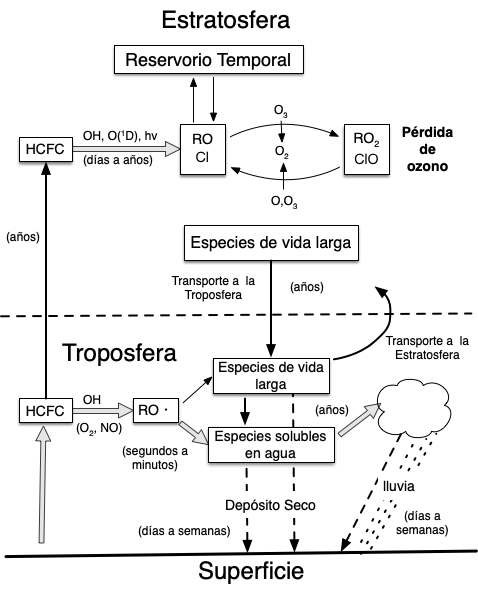
\includegraphics[width=0.95\textwidth]{halogenos_01.png}
\caption{Intercambio de hal\'ogenos en la atm\'osfera.}
\label{halo_01}
\end{center}
\end{figure}

% =============================================================================
% exercises/ejercicios_cap08.tex
% Ejercicios propuestos — Capítulo 7: Procesos Químicos en la Atmósfera
% =============================================================================

\section*{Ejercicios Propuestos}
\addcontentsline{toc}{section}{Ejercicios propuestos}
\label{sec:ejercicios_cap08}

\begin{bloque_ejercicios}[Ejercicios --- Cap\'{\i}tulo 7: Procesos Qu\'{\i}micos en la Atm\'osfera]

\begin{ejercicios}

% ----- Ejercicio 1: Oxidantes atmosféricos y cadena de oxidación ------------
\item Los tres principales oxidantes en la atm\'osfera son el radical
hidroxilo (\ce{OH^.}), el ozono (\ce{O3}) y el radical nitrato (\ce{NO3}).

\begin{enumerate}[label=\alph*)]
    \item Ordene los tres oxidantes de \textbf{mayor a menor} fuerza
          oxidante seg\'un se indica en el cap\'{\i}tulo e identifique en
          qu\'e per\'{\i}odo del d\'{\i}a (diurno o nocturno) domina
          cada uno como agente de remoci\'on de COV. Justifique.

    \item La producci\'on de \ce{OH^.} en la troposfera depende de la
          fotolisis del ozono. Escriba la secuencia de tres reacciones
          (denominadas \ref{RA}, \ref{RB} y \ref{RC} en el cap\'{\i}tulo)
          que llevan desde \ce{O3} hasta \ce{2OH^.}, e identifique
          en cu\'al de ellas interviene el vapor de agua.

    \item Usando la definici\'on de vida qu\'{\i}mica
          $\tau = 1/\left(k_{\ce{OH},i}\,[\ce{OH}]\right)$,
          explique por qu\'e el metano (\ce{CH4}, $\tau = 1837$~d)
          tiene una vida qu\'{\i}mica much\'{\i}simo mayor que
          el isopreno ($\tau = 2.8$~h) frente al mismo oxidante.
          ?`Qu\'e implica esto para su transporte global?

    \item Clasifique las cuatro etapas de una cadena de oxidaci\'on
          (iniciaci\'on, propagaci\'on, ramificaci\'on y terminaci\'on)
          e indique con un ejemplo tomado del cap\'{\i}tulo a qu\'e etapa
          corresponde la fotolisis del ozono (\ref{RA}).
\end{enumerate}

% ----- Ejercicio 2: Vida química de COV ------------------------------------
\item Con base en el \textbf{Cuadro~\ref{tvcov}} de vidas qu\'{\i}micas
de COV a \SI{298}{\kelvin}:

\begin{enumerate}[label=\alph*)]
    \item Reproduzca y complete la siguiente tabla indicando el oxidante
          \textbf{dominante} (el que produce la vida m\'as corta) para
          cada especie:

{%
\centering
\begin{tabular}{lcccl}
\toprule
\textbf{COV} & $\tau_{\ce{OH}}$ & $\tau_{\ce{O3}}$ &
$\tau_{\ce{NO3}}$ & \textbf{Oxidante dominante} \\
\midrule
Metano    & 1837 d & ---    & ---    & \\
Eteno     & 1.4 d  & 6.7 d  & 107 d  & \\
Propeno   & 10.6 h & 1.1 d  & 2.3 d  & \\
Isopreno  & 2.8 h  & 20.2 h & 45 min & \\
$\beta$-pineno & 3.5 h & 17.2 h & 12 min & \\
\bottomrule
\end{tabular}
\par
}%

    \item Para el propeno, calcule la constante de velocidad de segundo
          orden $k_{\ce{OH},\text{propeno}}$ sabiendo que la
          concentraci\'on t\'{\i}pica de \ce{OH^.} en la troposfera
          es $[\ce{OH}] = 1\times10^6$~mol\'eculas~cm$^{-3}$ y que
          $\tau_{\ce{OH}} = \SI{10.6}{\hour}$.
          \textit{Exprese el resultado en cm$^3$~mol\'ecula$^{-1}$~s$^{-1}$.}

    \item A partir de sus resultados, explique por qu\'e los terpenos
          bios\'{\i}nteticos (isopreno, $\beta$-pineno) son especialmente
          importantes en la formaci\'on de aerosoles org\'anicos
          secundarios en atm\'osferas forestales.
\end{enumerate}

\textit{[Respuesta parcial:
(b) $\tau = \SI{10.6}{\hour} = 38160$~s;
    $k_{\ce{OH}} = 1/(38160 \times 10^6)
    \approx 2.6\times10^{-11}$~cm$^3$~mol\'ecula$^{-1}$~s$^{-1}$]}

% ----- Ejercicio 3: Química del SO2 ----------------------------------------
\item La oxidaci\'on del \ce{SO2} en la atm\'osfera sigue varias rutas.

\begin{enumerate}[label=\alph*)]
    \item Escriba la secuencia completa de cuatro reacciones que
          convierten \ce{SO2} en \ce{H2SO4} v\'{\i}a reacci\'on
          en fase gaseosa con el radical \ce{OH^.}, tal como se
          describe en el cap\'{\i}tulo. Identifique en qu\'e paso se
          regenera el radical \ce{HO2^.}.

    \item Se establece que el tiempo de vida del \ce{SO2} frente a
          la reacci\'on con \ce{OH^.} es de aproximadamente una semana.
          Si la concentraci\'on de \ce{OH^.} es
          $[\ce{OH}] = 1\times10^6$~mol\'eculas~cm$^{-3}$,
          estime la constante de velocidad de segundo orden
          $k_{\ce{OH},\ce{SO2}}$.
          \textit{Use $\tau \approx 7$~d.}

    \item El DMS (\ce{CH3SCH3}) es el mayor contribuidor natural
          al flujo global de azufre. Describa:
          (i)~su fuente biol\'ogica principal,
          (ii)~los dos oxidantes que controlan su vida en atm\'osferas
          marinas, y
          (iii)~por qu\'e su remoci\'on presenta un ciclo diurno.

    \item El \ce{H2S} tiene un tiempo de vida de $\sim$70~h frente
          a \ce{OH^.}. Escriba la reacci\'on inicial de remoci\'on
          y el producto final al que eventualmente conduce seg\'un
          el cap\'{\i}tulo.
\end{enumerate}

\textit{[Respuesta parcial:
(b) $\tau = 7 \times 86400 = 604800$~s;
    $k = 1/(604800 \times 10^6)
    \approx 1.6\times10^{-12}$~cm$^3$~mol\'ecula$^{-1}$~s$^{-1}$]}

% ----- Ejercicio 4: Estado fotoestacionario del ozono troposférico ----------
\item El sistema \ce{NO2}/\ce{NO}/\ce{O3} en la troposfera alcanza un
estado fotoestacionario descrito por las reacciones \ref{RN1}--\ref{RN3}
del cap\'{\i}tulo. La concentraci\'on de ozono en el estado estacionario est\'a
dada por:
\[
    [\ce{O3}] = \frac{k_1[\ce{NO2}]}{k_3[\ce{NO}]}
\]
y, cuando $[\ce{O3}]_0 = [\ce{NO}]_0 = 0$, por la expresi\'on
\ref{RN10}:
\[
    [\ce{O3}] = \frac{1}{2}\left[\left(\frac{k_1}{k_3}\right)^2
    + \frac{4k_1}{k_3}[\ce{NO2}]_0\right]^{1/2}
    - \frac{k_1}{2k_3}
\]

\begin{enumerate}[label=\alph*)]
    \item Usando $k_1/k_3 = 10$~ppb y $[\ce{NO2}]_0 = 100$~ppb,
          calcule $[\ce{O3}]$ en el estado estacionario y verifique
          que coincide con el valor del \textbf{Cuadro~\ref{ozono_foto}}.

    \item Repita el c\'alculo con $[\ce{NO2}]_0 = 1000$~ppb y compare
          con el valor tabulado.

    \item Aplique la aproximaci\'on de estado seudo-estable (PSSA) al
          \'atomo de ox\'{\i}geno \ce{O^.} para deducir la
          expresi\'on~\ref{RN7}:
          \[
              [\ce{O}] = \frac{k_1[\ce{NO2}]}{k_2[\ce{O2}][\ce{M}]}
          \]
          Explique f\'{\i}sicamente por qu\'e esta aproximaci\'on es
          v\'alida para una especie tan reactiva como \ce{O^.}.

    \item El cap\'{\i}tulo concluye que las concentraciones de \ce{O3}
          observadas en atm\'osferas urbanas (hasta 120~ppb) son
          mayores que las calculadas con s\'olo las reacciones
          \ref{RN1}--\ref{RN3}. ?`Qu\'e tipo de compuestos y
          reacciones adicionales son necesarios para explicar este
          exceso?
\end{enumerate}

\textit{[Respuesta parcial:
(a) $[\ce{O3}] = \tfrac{1}{2}[(10^2 + 4\times10\times100)^{1/2}] - 5
    = \tfrac{1}{2}[2300^{1/2}] - 5
    \approx \tfrac{1}{2}(47.96) - 5 \approx 19\ldots\approx 27$~ppb $\checkmark$;
(b) $[\ce{O3}] \approx 95$~ppb $\checkmark$]}

% ----- Ejercicio 5: Aminas y compuestos de carbono -------------------------
\item Los compuestos nitrogenados y carbonados desempe\~nan roles clave
en la qu\'{\i}mica atmosf\'erica.

\begin{enumerate}[label=\alph*)]
    \item Escriba las tres reacciones de aminas con el radical \ce{OH^.}
          presentadas en el cap\'{\i}tulo (para \ce{NH3},
          \ce{CH3NH2} y \ce{(CH3)2NH}) e identifique el tipo de
          producto radical generado en cada caso.

    \item El amon\'{\i}aco (\ce{NH3}) reacciona preferentemente con
          \'acidos atmosf\'ericos antes que con \ce{OH^.}.
          Escriba la reacci\'on con el \ce{HNO3} gaseoso e identifique
          el producto s\'olido formado. ?`Qu\'e relevancia tiene esta
          reacci\'on para la formaci\'on de PM$_{2.5}$?

    \item Describa las tres rutas de formaci\'on de radicales org\'anicos
          a partir de compuestos de carbono seg\'un el cap\'{\i}tulo
          (ox\'{\i}geno singelete, radical hidroxilo y ozono),
          escribiendo la reacci\'on general de cada una
          usando \ce{RH} como hidrocarburo gen\'erico.

    \item El PAN (nitrato de peroxiacetil) es un componente caracter\'{\i}stico
          del esmog fotoqu\'{\i}mico. Describa la secuencia de tres
          pasos que lleva desde un aldeh\'{\i}do hasta el PAN,
          pasando por el radical peroxiacilo y su reacci\'on final con
          \ce{NO2}.
\end{enumerate}

% ----- Ejercicio 6: Halógenos y destrucción catalítica ---------------------
\item Los compuestos hal\'ogenos participan en ciclos catal\'{\i}ticos
de destrucci\'on de ozono.

\begin{enumerate}[label=\alph*)]
    \item La reacci\'on del \'atomo de Cl con hidrocarburos (reacci\'on
          \ref{RH1}) compite con su oxidaci\'on por \ce{O3}
          (reacci\'on \ref{RH2}). Seg\'un el cap\'{\i}tulo, la fracci\'on
          que reacciona con \ce{O3} en lugar de \ce{RH} es:
          F $\approx$ 0\% (F), 50\% (Cl), 99\% (Br) y 100\% (I).
          Explique cualitativamente esta tendencia en t\'erminos de la
          reactividad decreciente de los hal\'ogenos hacia compuestos
          que contienen H (HX).

    \item La reacci\'on del \ce{CH3Cl} con \ce{OH^.} libera finalmente
          un \'atomo de \ce{Cl^.}. Escriba la secuencia completa de
          tres reacciones indicadas en el cap\'{\i}tulo:
          \ce{CH3Cl + OH^. ->}, \ce{^.CH2Cl + O2 ->} y
          \ce{CH2ClOO^. + NO ->}.

    \item Describa c\'omo el \ce{HCl} generado en la estratosfera
          puede ser devuelto al ciclo activo del cloro (\ce{ClO_$x$})
          mediante la reacci\'on con el radical \ce{OH^.} (reacci\'on
          \ref{RH3}).

    \item Explique por qu\'e las constantes de velocidad de los \'atomos
          de Cl con hidrocarburos son significativamente mayores que las
          del \ce{OH^.} con los mismos compuestos, y qu\'e consecuencia
          tiene esto para la remoci\'on de hidrocarburos en zonas
          costeras con aerosol salino marino.
\end{enumerate}

% ----- Ejercicio 7: Balance de ozono estratosférico (Chapman) --------------
\item El balance natural de ozono en la estratosfera se describe mediante
las reacciones de Chapman.

\begin{enumerate}[label=\alph*)]
    \item Escriba las cuatro reacciones del mecanismo de Chapman:
          dos de formaci\'on (reacciones \ref{OE1} y \ref{OE2})
          y dos de destrucci\'on (reacci\'on \ref{OE3} y su reacci\'on
          inversa de regeneraci\'on). Indique las longitudes de onda
          de los fotones involucrados en cada fotolisis.

    \item Usando la analog\'{\i}a del ``balde que gotea'' descrita en
          el cap\'{\i}tulo, explique qu\'e condici\'on debe cumplirse para
          que el nivel de ozono permanezca constante, y qu\'e ocurre
          cuando se introducen compuestos adicionales como los CFC.

    \item El cap\'{\i}tulo indica que la concentraci\'on promedio de ozono
          es 300~DU, equivalente a una capa de \SI{3}{\milli\metre}.
          Si en el ``agujero'' ant\'artico cae a 100~DU:
          \begin{enumerate}[label=\roman*)]
              \item ?`Cu\'antos mil\'{\i}metros de espesor
                    representan 100~DU?
              \item Usando la definici\'on de que 1~DU $\equiv$
                    $2.69\times10^{16}$~mol\'eculas~cm$^{-2}$,
                    calcule el n\'umero total de mol\'eculas de
                    \ce{O3} en una columna de 1~cm$^2$ de base
                    para 300~DU y para 100~DU.
          \end{enumerate}

    \item La columna total de aire comprimido a STP tiene un espesor
          de \SI{8}{\kilo\metre}. Calcule qu\'e porcentaje del espesor
          total de la atm\'osfera representa la capa de ozono de 300~DU
          (\SI{3}{\milli\metre}).
\end{enumerate}

\textit{[Respuesta parcial:
(c-i) $100\,\text{DU} \rightarrow \SI{1}{\milli\metre}$;
(c-ii) $300\,\text{DU}: N = 300 \times 2.69\times10^{16}
      = 8.07\times10^{18}$~mol\'eculas~cm$^{-2}$;
      $100\,\text{DU}: N = 2.69\times10^{18}$~mol\'eculas~cm$^{-2}$;
(d) $3\,\text{mm}/8\,000\,000\,\text{mm} = 3.75\times10^{-7}$, es
    decir, $\sim 0.000038\%$ del espesor total]}

% ----- Ejercicio 8: Ciclos catalíticos de pérdida de ozono -----------------
\item Los ciclos catal\'{\i}ticos \ce{HO_$x$}, \ce{NO_$x$} y
\ce{ClO_$x$} son responsables de la p\'erdida acelerada de ozono
en la estratosfera.

\begin{enumerate}[label=\alph*)]
    \item Para el ciclo \ce{HO_$x$}, escriba las dos reacciones
          propagadoras (\ce{OH + O3} y \ce{HO2 + O3}) y la reacci\'on
          global neta. ?`Cu\'al es el cat\'alizador del ciclo?
          ?`C\'omo se termina el ciclo?

    \item Para el ciclo catal\'{\i}tico del \ce{NO_$x$}
          (reacciones \ref{R10}--\ref{R11}), escriba las dos
          reacciones y la reacci\'on neta. Calcule cu\'antas
          mol\'eculas de \ce{O_$x$} (equivalente a \ce{O3})
          se consumen por cada ciclo completo.

    \item El ciclo \ce{ClO_$x$} se inicia con la fotolisis del CFC-12
          (\ce{CF2Cl2}). Escriba:
          (i)~la reacci\'on de fotolisis del CFC-12,
          (ii)~las dos reacciones propagadoras del ciclo
          \ce{Cl}/\ce{ClO}, y
          (iii)~la reacci\'on neta global.

    \item Compare los tres ciclos catal\'{\i}ticos (\ce{HO_$x$},
          \ce{NO_$x$}, \ce{ClO_$x$}) llenando la siguiente tabla:

{%
\centering
\begin{tabular}{lccc}
\toprule
\textbf{Caracter\'{\i}stica} & \ce{HO_$x$} & \ce{NO_$x$} & \ce{ClO_$x$} \\
\midrule
Radical cat. & & & \\
Fuente principal & & & \\
Reacci\'on de terminaci\'on & & & \\
Reservorio inactivo & & & \\
\bottomrule
\end{tabular}
\par
}%
\end{enumerate}

% ----- Ejercicio 9: PSCs y agujero de ozono --------------------------------
\item Las nubes estratosf\'ericas polares (PSC) desempe\~nan un papel
fundamental en el agujero de ozono ant\'artico.

\begin{enumerate}[label=\alph*)]
    \item El cap\'{\i}tulo indica que las PSC se forman alrededor de
          \SI{-72}{\celsius}. Convierta esta temperatura a Kelvin
          y explique por qu\'e las PSC son m\'as frecuentes sobre
          la Ant\'artida que sobre el \'Artico.

    \item En la superficie de las PSC los gases de ``dep\'osito''
          \ce{HCl} y \ce{ClONO2} se activan. Escriba la reacci\'on
          heterog\'enea de \ce{N2O5} con \ce{NaCl} en aerosol salino
          que produce una especie activa de cloro (\ce{XNO2}) y una sal
          s\'olida, seg\'un el cap\'{\i}tulo.

    \item La reacci\'on \ce{N2O + O(^1D) -> 2NO} en la estratosfera
          es responsable del 5\% de la p\'erdida del \ce{N2O}.
          Si la tasa total de p\'erdida de \ce{N2O} es
          $F = \SI{1.0e10}{\kilo\gram}/$a\~no, ?`cu\'anta masa
          (en kg/a\~no) se convierte a NO por esta v\'{\i}a?
          ?`Qu\'e ocurre con el 95\% restante?

    \item Molina y Rowland recibieron el Premio Nobel de Qu\'{\i}mica
          en 1995 junto con Paul Crutzen. Explique la contribuci\'on
          espec\'{\i}fica de cada uno en la comprensi\'on de la
          destrucci\'on del ozono estratosf\'erico, con base en la
          informaci\'on del cap\'{\i}tulo.
\end{enumerate}

\textit{[Respuesta parcial:
(a) \SI{-72}{\celsius} $= \SI{201}{\kelvin}$;
(c) $5\%$ de $10^{10}$ kg/a\~no $= 5\times10^8$~kg/a\~no;
    el 95\% se convierte en \ce{N2} (inerte) por fotolisis y  oxidaci\'on con \ce{O(^1D)}]}

% ----- Ejercicio 10 (avanzado): Ciclo 2 de ClO y ecuación de continuidad ---
\item \textbf{[Avanzado]} El cap\'{\i}tulo describe tres ciclos de
destrucci\'on de ozono con hal\'ogenos (\textbf{Cuadro~\ref{desozo}}).

\begin{enumerate}[label=\alph*)]
    \item Para el \textbf{Ciclo 2} (\ce{ClO + ClO -> (ClO)2 -> \ldots}),
          escriba los cuatro pasos elementales y la reacci\'on global
          neta. Identifique cu\'al paso requiere un fot\'on ($h\nu$)
          y cu\'al produce el \'atomo de Cl libre necesario para
          continuar el ciclo.

    \item Para el \textbf{Ciclo 3} (que involucra tanto Cl como Br),
          escriba los cuatro pasos y la reacci\'on neta.
          Compare la eficiencia del Ciclo 3 con la del Ciclo 1
          en t\'erminos de la raz\'on de mol\'eculas de \ce{O3}
          destruidas por \'atomo de hal\'ogeno.

    \item La ecuaci\'on de continuidad del ozono estratosf\'erico es:
          \[
              \frac{\partial[\ce{O3}]}{\partial t}
              = P - L - \nabla\cdot(\vec{v}[\ce{O3}])
          \]
          Identifique cada t\'ermino f\'{\i}sicamente e indique
          qu\'e proceso representa cada uno:
          \begin{enumerate}[label=\roman*)]
              \item el t\'ermino $P$,
              \item el t\'ermino $L$,
              \item el t\'ermino $\nabla\cdot(\vec{v}[\ce{O3}])$.
          \end{enumerate}
          ?`En qu\'e regi\'on de la Tierra domina el transporte
          advectivo sobre la producci\'on qu\'{\i}mica?

    \item La circulaci\'on de Brewer-Dobson transporta \ce{O3} desde
          los tr\'opicos hacia los polos. Explique por qu\'e, a pesar
          de que el \ce{O3} se produce principalmente en la estratosfera
          tropical, las m\'aximas concentraciones se observan en
          latitudes altas (salvo en la Ant\'artida en primavera austral).
\end{enumerate}

\end{ejercicios}

\end{bloque_ejercicios}
% =============================================================================
% FIN DE ejercicios_cap08.tex
% =============================================================================



   
%  
%                 ESTRATOSFERA
%  

\chapter[Quimica en la estratosfera]{Qu\'{\i}mica en la estratosfera}
\label{c:estrato}
\index{estratosfera!quimica@qu\'{\i}mica}

El ozono estratosf\'erico (\ce{O3}), descrito previamente en la secci\'on \ref{esozono}, constituye un componente cr\'{\i}tico para la biosfera terrestre al absorber el 97-99\% de la radiaci\'on ultravioleta (UV-B/C) solar. Su formaci\'on y destrucci\'on din\'amica, as\'{\i} como su distribuci\'on espacial, representan procesos fundamentales para comprender tanto el origen de la vida en el planeta como las amenazas actuales a este escudo protector. Este cap\'{\i}tulo aborda los mecanismos qu\'{\i}micos que gobiernan su equilibrio natural y las perturbaciones antropog\'enicas que alteran dicho balance.

En la  Secci\'on~\ref{dvozono}, se analiza la \textbf{distribuci\'on vertical y latitudinal del ozono}, caracterizada por:
\begin{itemize}
    \item M\'axima concentraci\'on entre \SIrange{20}{30}{\kilo\metre}  de altitud (Capa de Ozono)
    \item Variaciones estacionales (agotamiento polar en primavera austral)
    \item Gradientes latitudinales influenciados por la circulaci\'on de Brewer-Dobson
\end{itemize}

La Secci\'on~\ref{oestra} explora el \textbf{balance fotoqu\'{\i}mico del ozono}, donde se integran las reacciones de Chapman:
\begin{itemize}
    \item Formaci\'on: \ce{O2 + h$\nu$ ->[ $\lambda < \SI{242}{\nano\metre}$] 2O} seguido de \ce{O + O2 ->[M] O3 }
    \item Destrucci\'on natural: \ce{O3 + h$\nu$  ->[$\lambda < \SI{310}{\nano\metre}$] O2 + O} 
\end{itemize}

La Secci\'on~\ref{cpeoz} detalla los \textbf{ciclos de p\'erdida catal\'{\i}tica}, mecanismos aceleradores que explican el agotamiento observado desde 1980:
\begin{itemize}
    \item \textbf{Radicales hidroxilo} (\ref{roh}): Ciclo HO$_x$ con reacciones tipo \ce{HO^. + O3 -> HO2^. + O2}
    \item \textbf{Radicales de nitr\'ogeno} (\ref{rno3}): Ciclo NO$_x$ catalizado por \ce{NO^.} de origen natural y antropog\'enico
    \item \textbf{Radicales de cloro} (\ref{rclo}): Ciclo ClO$_x$ activado por CFCs, con reacciones catalizadas en las superficies de las \gls{PSC}s (Nubes Estratosf\'ericas Polares)\index{PSC}
\end{itemize}

Finalmente, se discuten las \textbf{unidades Dobson (\gls{DU})}, est\'andar global para cuantificar el ozono total atmosf\'erico, vinculando las mediciones satelitales con los modelos qu\'{\i}micos presentados. Estos conceptos, junto con los efectos en salud descritos en \ref{o3_salud}, proveen un marco integral para evaluar pol\'{\i}ticas de protecci\'on de la capa de ozono y mitigaci\'on de sustancias agotadoras.

\section{Distribuci\'on de ozono}
\label{dvozono}
Los gradientes latitudinales de ozono estratosf\'erico est\'an profundamente influenciados por la \textbf{circulaci\'on de Brewer-Dobson},\index{circulacion@circulaci\'on!Brewer-Dobson} un sistema de transporte meridional que domina la din\'amica de la estratosfera. Este patr\'on de circulaci\'on, impulsado por ondas planetarias y turbulencia en la tropopausa, transporta masa y especies qu\'{\i}micas desde los tr\'opicos hacia los polos en direcci\'on vertical y horizontal. El ozono (\ce{O3}), producido principalmente en la estratosfera tropical por fot\'olisis de \ce{O2} reacci\'on: \ce{O2 + h$\nu$ -> 2O} ($\lambda < \SI{242}{\nano\metre}$), es arrastrado hacia latitudes medias y polares mediante este mecanismo. Sin embargo, la eficiencia del transporte var\'{\i}a estacionalmente, siendo m\'as intenso durante el invierno y primavera boreales, lo que explica:

\begin{itemize}
    \item M\'aximas concentraciones de ozono en latitudes altas ($>60^\circ$), excepto en la Ant\'artida durante la primavera austral debido al agujero polar (ver Secci\'on \ref{esozono}).
    \item Un gradiente de concentraci\'on decreciente desde los polos hacia el ecuador en capas superiores ($\sim\SI{30}{\kilo\metre}$), invertido en capas bajas ($\sim\SI{15}{\kilo\metre}$) por procesos de destrucci\'on catal\'{\i}tica.
    \item Asimetr\'{\i}as hemisf\'ericas: mayores valores en el hemisferio norte por interacciones con ondas orogr\'aficas y mayor actividad de ondas planetarias.
\end{itemize}

La ecuaci\'on de continuidad para el ozono estratosf\'erico refleja este balance:
\begin{equation}
\frac{\partial [\ce{O3}]}{\partial t} = P - L - \nabla \cdot (\vec{v}[\ce{O3}])
\end{equation}
donde \( P \) y \( L \) son las tasas de producci\'on y p\'erdida qu\'{\i}mica, y \( \nabla \cdot (\vec{v}[\ce{O3}]) \) representa el transporte advectivo por la circulaci\'on de Brewer-Dobson. Este mecanismo no solo distribuye el ozono, sino que tambi\'en modula la exposici\'on a UV-B en superficie, con implicaciones clim\'aticas y biol\'ogicas globales.

El ozono (\ce{O3}) es una mol\'ecula relativamente inestable formada por tres \'atomos de ox\'{\i}geno (O) ver \textbf{Figura~\ref{reso3}}. Aunque representa s\'olo una peque\~na fracci\'on de la atm\'osfera, el ozono es crucial para la vida en la Tierra.
\begin{figure}[htbp]
\begin{center}
\ce{O\bond{=}O\bond{-}O <--> O\bond{-}O\bond{=}O } 
\caption{Mol\'ecula de ozono y su resonancia}
\label{reso3}
\end{center}
\end{figure}


Dependiendo de d\'onde resida el ozono, puede proteger o da\~nar la vida en la Tierra. La mayor parte del ozono reside en la estratosfera (una capa de la atm\'osfera entre $10$ y \SI{40}{\kilo\metre}  por encima de nosotros), donde act\'ua como un escudo para proteger la superficie de la Tierra de la da\~nina radiaci\'on ultravioleta del Sol. Con un debilitamiento de este escudo, ser\'{\i}amos m\'as susceptibles al c\'ancer de piel, cataratas y sistemas inmunol\'ogicos deteriorados. M\'as cerca de la Tierra, en la troposfera (la capa atmosf\'erica desde la superficie hasta unos \SI{10}{\kilo\metre}), el ozono es un contaminante nocivo que da\~na el tejido pulmonar y las plantas.

\section{Balance de ozono en la estratosfera}\label{oestra}
\index{ozono!estratosfera}

En la estratosfera, el ozono se crea principalmente por la radiaci\'on ultravioleta. Cuando los rayos ultravioleta de alta energ\'{\i}a inciden en las mol\'eculas de ox\'{\i}geno ordinarias (\ce{O2}), las dividen en dos \'atomos de ox\'{\i}geno \'unicos, conocidos como ox\'{\i}geno at\'omico.
\reaction{ O2 + h$\nu$ -> 2O^. \label{OE1}}
\reaction{ O2 + O^. + M -> O3 + M \label{OE2}}
 Luego, un \'atomo de ox\'{\i}geno liberado se combina con otra mol\'ecula de ox\'{\i}geno para formar una mol\'ecula de ozono. Hay tanto ox\'{\i}geno en nuestra atm\'osfera que estos rayos ultravioleta de alta energ\'{\i}a son completamente absorbidos en la estratosfera.

El ozono es extremadamente valioso ya que absorbe una variedad de energ\'{\i}a ultravioleta. Cuando una mol\'ecula de ozono absorbe incluso radiaci\'on ultravioleta de baja energ\'{\i}a, se divide en una mol\'ecula de ox\'{\i}geno ordinaria y un \'atomo de ox\'{\i}geno libre. Por lo general, este \'atomo de ox\'{\i}geno libre se vuelve a unir r\'apidamente con una mol\'ecula de ox\'{\i}geno para formar otra mol\'ecula de ozono. Debido a este ´´ciclo ozono-ox\'{\i}geno'', la  radiaci\'on ultravioleta da\~nina se convierte continuamente en calor.
\reaction{ O3 + h$\nu$ -> O2 +O^. \label{OE3}}
\reaction*{  O^. + O2 ->  O3  }
Las reacciones naturales distintas del ``ciclo ozono-ox\'{\i}geno'' descrito anteriormente tambi\'en afectan la concentraci\'on de ozono en la estratosfera. Debido a que el ozono y los \'atomos de ox\'{\i}geno libres son muy inestables, reaccionan muy f\'acilmente con los compuestos de nitr\'ogeno, hidr\'ogeno, cloro y bromo que se encuentran naturalmente en la atm\'osfera de la Tierra (liberados tanto de fuentes terrestres como oce\'anicas). Por ejemplo, los \'atomos individuales de cloro pueden convertir el ozono en mol\'eculas de ox\'{\i}geno y esta p\'erdida de ozono equilibra la producci\'on de ozono mediante rayos ultravioleta de alta energ\'{\i}a que inciden en las mol\'eculas de ox\'{\i}geno.
\begin{eqnarray*}
 &\ce{Cl + O3 & -> ClO + O2  \\
 &ClO +  O^.  & -> Cl + O2 }\\ 
  \mathrm{Neto: } &\ce{O3 + O^.  &  -> 2O2}
\end{eqnarray*}
Adem\'as del equilibrio natural del ozono, los cient\'{\i}ficos han descubierto que los niveles de ozono cambian peri\'odicamente como parte de ciclos naturales regulares, como el cambio de estaciones, los vientos y las variaciones solares a largo plazo. Adem\'as, las erupciones volc\'anicas pueden inyectar materiales en la estratosfera que pueden provocar una mayor destrucci\'on del ozono.

A lo largo de la vida de la Tierra, los procesos naturales han regulado el equilibrio del ozono en la estratosfera. Una forma sencilla de comprender el equilibrio del ozono es pensar en un balde que gotea. Siempre que se vierta agua en el balde al mismo ritmo que se escapa, la cantidad o el nivel de agua en el balde seguir\'a siendo el mismo. Del mismo modo, mientras el ozono se cree al mismo ritmo que se destruye, la cantidad total de ozono seguir\'a siendo la misma.

Sin embargo, a partir de principios de los a\~nos 1970, los cient\'{\i}ficos encontraron pruebas de que las actividades humanas estaban alterando el equilibrio del ozono. La producci\'on humana de sustancias qu\'{\i}micas que contienen cloro, como los clorofluorocarbonos (CFC), ha a\~nadido un factor adicional que destruye el ozono. Los CFC son compuestos formados por cloro, fl\'uor y carbono unidos entre s\'{\i}. Debido a que son mol\'eculas extremadamente estables, los CFC no reaccionan f\'acilmente con otras sustancias qu\'{\i}micas de la atm\'osfera inferior. Una de las pocas fuerzas que pueden romper las mol\'eculas de CFC es la radiaci\'on ultravioleta. En la atm\'osfera inferior, los CFC est\'an protegidos de la radiaci\'on ultravioleta por la propia capa de ozono. De este modo, las mol\'eculas de CFC pueden migrar intactas a la estratosfera. Aunque las mol\'eculas de CFC son m\'as pesadas que el aire, las corrientes de aire y los procesos de mezcla de la atm\'osfera las transportan a la estratosfera.

Una vez en la estratosfera, las mol\'eculas de CFC ya no est\'an protegidas de la radiaci\'on ultravioleta por la capa de ozono. Bombardeadas por la energ\'{\i}a ultravioleta del sol, las mol\'eculas de CFC se descomponen y liberan \'atomos de cloro. Luego, los \'atomos de cloro libre reaccionan con las mol\'eculas de ozono, tomando un \'atomo de ox\'{\i}geno para formar mon\'oxido de cloro y dejando una mol\'ecula de ox\'{\i}geno ordinaria.

Si cada \'atomo de cloro liberado por una mol\'ecula de CFC destruyera s\'olo una mol\'ecula de ozono, los CFC representar\'{\i}an muy poca amenaza para la capa de ozono. Sin embargo, cuando una mol\'ecula de mon\'oxido de cloro encuentra un \'atomo libre de ox\'{\i}geno, el \'atomo de ox\'{\i}geno rompe el mon\'oxido de cloro, roba el \'atomo de ox\'{\i}geno y libera el \'atomo de cloro nuevamente a la estratosfera para destruir m\'as ozono. Esta reacci\'on ocurre una y otra vez, permitiendo que un solo \'atomo de cloro act\'ue como catalizador, destruyendo muchas mol\'eculas de ozono.

Afortunadamente, los \'atomos de cloro no permanecen en la estratosfera para siempre. Cuando un \'atomo de cloro libre reacciona con gases como el metano (\ce{CH4}), se une a una mol\'ecula de cloruro de hidr\'ogeno (HCl), que puede transportarse hacia abajo desde la estratosfera hasta la troposfera, donde puede ser arrastrado por la lluvia. Por lo tanto, si los humanos dejan de colocar CFC y otras sustancias qu\'{\i}micas que destruyen la capa de ozono en la estratosfera, la capa de ozono eventualmente podr\'{\i}a repararse a s\'{\i} misma.

\section[Ciclos de perdida catalitica]{Ciclos de p\'erdida catal\'{\i}tica}
\label{cpeoz}

\subsection{Radicales hidroxilo}\index{radical!hidroxilo}
\label{roh}

Se descubri\'o en los a\~nos 1950 que los ciclos iniciados por la oxidaci\'on del vapor de agua pueden representar un sumidero importante de ozono en la estratosfera. El vapor de agua se suministra a la estratosfera por el transporte y oxidaci\'on del metano (\ce{CH4}). El vapor de agua en estratosfera es relativamente uniforme, en el intervalo de $3-5$ ppm. En la estratosfera el vapor de agua se oxida por el \ce{O(^1D)} producido por:
\reaction{H2O + O(^1D)  ->  2OH \label{OHr1}}
Los \'atomos de alta energ\'{\i}a \ce{O(^1D)} son necesario para superar la estabilidad del la mol\'ecula de agua.

El radical hidr\'oxido (OH)  producido puede reacciona con el \ce{O3}, produciendo el radial hidroperoxi (\ce{HO2}), el cual reacciona con el \ce{O3}.
\begin{eqnarray*}
& \ce{OH + O3    & -> HO2 + O2 \\
      & HO2 +  O3   &-> OH + 2O2} \\
\mathrm{Neto: } &  \ce{2O3   &  ->  3O2}
\end{eqnarray*}

El conjunto OH y \ce{HO2} se conoce como la familia \ce{HO_$x$}.\index{familia!\ce{HO_$x$}}

Las reacciones anteriores consumen el \ce{O3} conservando el \ce{HO_$x$}. Por lo tanto el \ce{HO_$x$} act\'ua como catalizador para la p\'erdida de \ce{O3}. La producci\'on de una mol\'ecula de \ce{HO_$x$} puede resultar en la p\'erdida de un gran n\'umero de mol\'eculas de \ce{O3} por el ciclado del \ce{HO_$x$}. La terminaci\'on de este ciclo catal\'{\i}tico requiere de la p\'erdida del \ce{HO_$x$}, por una reacci\'on como:
\reaction*{OH + HO2 -> H2O + O2}

\subsection{Radicales de nitr\'ogeno}\index{radical!de nitr\'ogeno}\label{rno3}
Un avance en la compresi\'on del  \ce{O3}  estratosf\'erico se obtuvo en los EEUU y otros pa\'{\i}ses involucrados en el lanzamiento de un avi\'on supers\'onico que volaba en la estratosfera.  Se realiz\'o una evaluaci\'on las emisiones de estos aviones en la capa de \ce{O3}.  Un componente importante en la emisi\'on es el \'oxido n\'{\i}trico (NO) , formado por al oxidaci\'on del \ce{N2} a altas temperatura en el motor del avi\'on. En la estratosfera el NO reacciona r\'apidamente con el \ce{O3}, para producir  \ce{NO2} , que luego se fotoliza:
\begin{eqnarray*}
 \ce{NO + O3       & -> &NO2 + O2 \\
  NO2 +  h$\nu$  &  -> &NO + O^. \\
   O^. + O2          &  ->[M] & O3}
\end{eqnarray*}


Este ciclo entre el NO y \ce{NO2} tiene lugar en una escala de tiempo de 1 minuto durante el d\'{\i}a. No tiene un efecto neto en el \ce{O3} y se denomina como ciclo nulo\index{ozono!ciclo nulo}. Este causa, sin embargo, un intercambio r\'apido entre el NO y \ce{NO2}. Nos referimos al conjunto de NO y \ce{NO2} como \ce{NO_$x$}.

Investigaciones posteriores de la qu\'{\i}mica del \ce{NO_$x$} en la estratosfera mostraron que una fracci\'on de mol\'eculas de \ce{NO2} reacciona con \'atomos de ox\'{\i}geno 

\reaction*{NO2 + O^. -> NO + O2}

La secuencia de reacciones del N representa el ciclo catal\'{\i}tico para la p\'erdida del ozono \ce{O3} ser\'{\i}an:
\begin{eqnarray}
            & \ce{NO + O3     &->   NO2 + O2} \label{R10} \\
            &\ce{NO2 +  O^.   & ->   NO + O2 } \label{R11} \\
  \mathrm{Neto: } &\ce{O3 + O^.  &->  2O2}\nonumber 
\end{eqnarray}

Cada ciclo consume dos mol\'eculas \ce{O_$x$} , que es equivalente a dos mol\'eculas de \ce{O3}. El paso importante es en la velocidad de~\ref{R11}

La terminaci\'on del ciclo catal\'{\i}tico involucra la p\'erdida de los radicales \ce{NO_$x$}. En el d\'{\i}a,  \ce{NO_$x$}, se oxida a  \ce{HNO3} por medio de radical OH que es un oxidante fuerte.
\reaction*{NO2 + OH ->[M] HNO3}
Durante la noche el OH esta ausente, debido a que no hay \ce{O(^ID)} para oxidar el \ce{H2O}. La p\'erdida de  \ce{NO_$x$} durante la noche tiene lugar mediante la oxidaci\'on del \ce{NO2} con \ce{O3} y la subsecuente conversi\'on del radical \ce{NO3 } a \ce{N2O5}:
\begin{eqnarray*}
 \ce{NO2 + O3    & ->       & NO3 + O2 \\
       NO3+ NO2  &  ->[M] & N2O5}
\end{eqnarray*}

La formaci\'on del \ce{N2O5} s\'olo tiene lugar durante la noche, debido a que durante el d\'{\i}a el \ce{NO3} se fotoliza hacia el \ce{NO2} en una escala de tiempo de unos segundos.

Los productos de oxidaci\'on del \ce{NO_$x$}, \ce{HNO3} y \ce{N2O5}, son especies no radicales y tiene un tiempo de vida relativamente largos con respecto a la perdida qu\'{\i}mica (semanas para el \ce{HNO3}, horas a d\'{\i}as para el \ce{N2O5}). 
\begin{eqnarray*}
 \ce{HNO3 + h$\nu$   & ->   & NO2 + OH \\
       HNO3 + OH        &  ->  & NO3 + H2O\\
       NO3  + h$\nu$    & ->   & NO2 + O\\
       N2O5 + h$\nu$   & ->   & NO3 + NO2}
\end{eqnarray*}
Estos eventualmente se convierten en \'oxidos de nitr\'ogeno  \ce{NO_$x$}
y sirven como almacenamiento de \ce{NO_$x$}. Se puede referir al conjunto \ce{NO_$x$} y sus reservas como otras familia qu\'{\i}mica, \ce{NO_$y$}. Finalmente la remoci\'on del \ce{NO_$y$} es por transporte a la troposfera donde el \ce{HNO3} se remueve r\'apidamente por deposito.\index{familia!\ce{NO_$y$}}

La identificaci\'on del mecanismo canalizado por \ce{NO_$x$} para la p\'erdida de \ce{O3} se volvi\'o una pista cr\'{\i}tica para identificar el sumidero faltante del \ce{O3} en el mecanismo de Chapman\index{Chapman@\textbf{Chapman}}.

Trabajos posteriores identificaron que el \ce{N2O}, es un producto de bajo rendimiento de los procesos de nitrificaci\'on-desnitrificaci\'on, la biosfera es fuente de este compuesto. El \ce{N2O} es una mol\'ecula estable que no posee sumideros en la troposfera. Por lo que es transportado a la estratosfera donde se encuentra con las altas concentraciones de \ce{O(^1D)}, permitiendo la oxidaci\'on a NO:

\reaction{N2O + O(^1D) -> 2NO}
esta reacci\'on es el 5\% de la p\'erdida del \ce{N2O}  en la estratosfera; el restante 95\% es convertido a \ce{N2} por la fot\'olisis y oxidaci\'on con  \ce{O(^1D)}  por una via alternativa. Sin embargo, la conversi\'on a \ce{N2} no tiene ning\'un inter\'es en la qu\'{\i}mica estratosf\'erica.

\subsection{Radicales de cloro}\index{radical!de cloro}\label{rclo}
En 1974, Mario Molina\index{molina@\textbf{Molina, Mario}} y Sherwood Roland\index{sherwood@\textbf{Roland, Sherwood}} indicaron el potencial de la p\'erdida de \ce{O3} asociada al incremento de las concentraciones atmosf\'ericas de cloroflourocarbonos (CFCs)\index{CFC}\index{cloroflourocarbonos}. Los CFCs no se encuentran en la naturaleza \'estos se manufacturan con prop\'ositos industriales en los 1930's  y su uso se increment\'o r\'apidamente en las siguientes d\'ecadas. Durante los 1970's y 1980's las concentraciones atmosf\'ericas de los CFCs rozaron 2--4\% al a\~no. Las mol\'eculas de CFC son inertes en la troposfera,  as\'{\i} son transportados a la estratosfera donde se fotolizan y liberan \'atomos de Cl. Por ejemplo, en el caso de \ce{CF2Cl2} (conocido como CFC-12) \index{CFC-12}
\reaction{CF2Cl2 +  h$\nu$ -> CF2Cl + Cl^.}

Los \'atomos de Cl  desencadenan el mecanismo de p\'erdida catal\'{\i}tica para el \ce{O3} involucrando un ciclo entre Cl y ClO (la familia \ce{ClO_$x$})la secuencia es similar a la del mecanismo catalizado con \ce{NO_$x$} (\ref{R11}):
\begin{eqnarray*}
            & \ce{Cl + O3     &->   ClO + O2}  \\
            &\ce{ClO +  O^.   & ->   Cl + O2 }  \\
  \mathrm{Neto: } &\ce{O3 + O^.   &->  2O2} 
\end{eqnarray*}

La terminaci\'on de \'este ciclo catal\'{\i}tico es mediante la conversi\'on del \ce{ClO_$x$} a un reservorio de cloro no-radical, HCl y \ce{ClNO3}:
\begin{eqnarray*}
 \ce{Cl + CH4   & ->   & HCl + CH3 \\
       ClO + NO2        &  ->[M]  & ClNO3}
\end{eqnarray*}

El tiempo de vida del HCl es t\'{\i}picamente unas pocas semanas y la del \ce{ClNO3} en el orden de un d\'{\i}a. Eventualmente estos repertorios se convierten en \ce{ClO_$x$}.
\begin{eqnarray*}
 \ce{HCl + OH   & ->   & Cl + H2O \\
       ClNO3 +   h$\nu$   &  ->  & Cl + NO3}
\end{eqnarray*}
Se define a la familia qu\'{\i}mica \ce{ClO_$y$} como la suma de \ce{ClO_$x$} m\'as sus reservorios.  \index{familia!\ce{ClO_$x$}} 

Molina y Rowland alertaron que la p\'erdida de \ce{O3}  catalizada con \ce{ClO_$x$}  podr\'{\i}a convertirse en una amenaza para la capa de \ce{O3}  en la medida de las concentraciones de CFC se incrementasen. Por sus trabajos relacionados a la p\'erdida de ozono en la estratosfera y el descubrimiento del hoyo de ozono compartieron el premio Nobel de qu\'{\i}mica en 1995 con Paul Crutzen\index{Crutzen@\textbf{Crutzen,Paul}}.

\section{Agotamiento del ozono estratosf\'erico}

El t\'ermino  ``agotamiento del ozono''\index{ozono!agotamiento} significa m\'as que simplemente la destrucci\'on natural del ozono: significa que la p\'erdida de ozono excede la creaci\'on de ozono (\textbf{Cuadro\,\ref{desozo}}). Piense de nuevo en el ``balde que gotea''. Poner en la atm\'osfera compuestos adicionales que destruyen el ozono, como los CFC, es como aumentar el tama\~no de los agujeros en nuestro ``cubeta'' de ozono. Los agujeros m\'as grandes hacen que el ozono se escape a un ritmo m\'as r\'apido del que se crea. En consecuencia, disminuye el nivel de ozono que nos protege de la radiaci\'on ultravioleta.
\begin{table}[htb]
\caption{Ciclos de destrucci\'on de ozono con hal\'ogenos}
\begin{center}
\begin{tabular}{rcl}
\multicolumn{3}{l}{\large\bfseries Ciclo 1 Destrucci\'on de Ozono}\\
\ce{Cl + O3} & \ce{ -> } &\ce{ClO + O2}\\
\ce{ClO + O^. } & \ce{ -> } &\ce{Cl + O2}\\\hline
 Neto: \ce{O3 + O^.} & \ce{ -> } & \ce{2O2}\\
\multicolumn{3}{l}{\large\bfseries Ciclo 2}\\
 \ce{ClO + ClO }          & \ce{ -> } &\ce{(ClO)_2}\\
 \ce{(ClO)_2 + h$\nu$ } & \ce{ -> } &\ce{ClOO^. + Cl}\\
 \ce{ClOO^. }                  & \ce{ -> } &\ce{Cl + O2}\\
 \ce{2(Cl + O3 ) }             & \ce{ -> } &\ce{ClO + O2}\\ \hline
 Neto: \ce{2O3} & \ce{ -> } & \ce{3O2}\\
\multicolumn{3}{l}{\large\bfseries Ciclo 3}\\
 \ce{ClO + BrO }          & \ce{ -> } &\ce{Cl + Br + O2}\\
 \ce{BrCl +  h$\nu$ }    & \ce{ -> } &\ce{Cl + Br }\\
 \ce{Cl +  O3 }    & \ce{ -> } &\ce{ClO + O2 }\\
 \ce{Br +  O3 }    & \ce{ -> } &\ce{BrO + O2 }\\\hline
 Neto: \ce{2O3} & \ce{ -> } & \ce{3O2}\\
\end{tabular}
\end{center}
\label{desozo}
\end{table}%
Durante los \'ultimos 15 a\~nos se ha descubierto en las zonas de la Ant\'artida y el \'Artico un mecanismo adicional que destruye r\'apidamente el ozono. Sobre los polos de la Tierra durante sus respectivos inviernos, la estratosfera se enfr\'{\i}a a temperaturas muy fr\'{\i}as y se forman nubes estratosf\'ericas polares (PSC).\index{PSC} En la estratosfera polar, casi todo el cloro se encuentra en forma de gases inactivos o ``de dep\'osito'', como el cloruro de hidr\'ogeno (HCl) y el nitrato de cloro (\ce{ClONO2}), que no reaccionan con el ozono ni entre s\'{\i}. Sin embargo, las reacciones qu\'{\i}micas de estos gases de cloro ``de dep\'osito''  pueden ocurrir en las superficies de las part\'{\i}culas de las nubes estratosf\'ericas polares, convirtiendo los gases de cloro en formas muy reactivas que destruyen r\'apidamente el ozono. Esta ``qu\'{\i}mica polar'' en las part\'{\i}culas de las nubes estratosf\'ericas ha provocado grandes disminuciones en las concentraciones de ozono sobre la Ant\'artida y el \'Artico. De hecho, los niveles de ozono caen tan bajo en primavera sobre la Ant\'artida que los cient\'{\i}ficos describen esta p\'erdida como el ``Agujero de Ozono Ant\'artico''.\index{ozono!agujero}

La formaci\'on de nubes estratosf\'ericas se da alrededor de los \SI{-72}{\celsius}  as\'{\i} en el polo sur es m\'as probable que se formen que en el polo norte por las temperaturas que se alcanzan.

As\'{\i} en las capas donde se tienen nubes estratosf\'ericas polares podemos encontrar que el ozono se ve reducido.

\subsection{Medici\'on de ozono en columna}
La Unidad Dobson\index{unidades!Dobson} (en ingl\'es, DU) es la unidad m\'as com\'un para medir la cantidad presente de ozono en la atm\'osfera terrestre. Una unidad Dobson es la cantidad de mol\'eculas de ozono que se necesitar\'{\i}an para crear una capa de ozono puro de 0.01 mil\'{\i}metros de espesor a una temperatura de 0 grados Celsius y una presi\'on de 1 atm\'osfera (la presi\'on del aire en la superficie de la Tierra). Expresado de otra manera, una columna de aire con una concentraci\'on de ozono de 1 unidad Dobson contendr\'{\i}a aproximadamente $2.69\times10^{16}$ mol\'eculas de ozono en una columna de un cent\'{\i}metro cuadrado de \'area en la base. Sobre la superficie de la Tierra, el espesor medio de la capa de ozono es de unas 300 unidades Dobson o una capa de 3 mil\'{\i}metros de espesor.

El ozono en la atm\'osfera no est\'a todo empaquetado en una sola capa a una cierta altitud sobre la superficie de la Tierra; est\'a disperso. Incluso el ozono estratosf\'erico conocido como ``la capa de ozono'' no es una sola capa de ozono puro. Es simplemente una regi\'on donde el ozono es m\'as com\'un que en otras altitudes. Los sensores satelitales y otros dispositivos de medici\'on del ozono miden la concentraci\'on total de ozono para una columna completa de la atm\'osfera. La Unidad Dobson es una forma de describir cu\'anto ozono habr\'{\i}a en la columna si estuviera todo comprimido en una sola capa.

La cantidad promedio de ozono en la atm\'osfera es de aproximadamente 300 unidades Dobson, equivalente a una capa de 3 mil\'{\i}metros de espesor, la altura de 2 centavos apilados. Lo que los cient\'{\i}ficos llaman el ``agujero'' de ozono ant\'artico es un \'area donde la concentraci\'on de ozono cae a un promedio de aproximadamente 100 unidades Dobson. Cien unidades Dobson de ozono formar\'{\i}an una capa de s\'olo 1 mil\'{\i}metro de espesor si se comprimieran en una sola capa, aproximadamente de la altura de una moneda de diez centavos.

\textquestiondown Cu\'anto es esto en comparaci\'on con el resto de la atm\'osfera?  Si todo el aire de una columna vertical que se extiende desde el suelo hasta el espacio fuera recolectado y comprimido a una temperatura de 0 grados Celsius y una presi\'on de 1 atm\'osfera, esa columna tendr\'{\i}a \SI{8}{\kilo\metre} de espesor. Al compararse con los \SI{3}{\milli\metre} descritos anteriormente y con esto uno se da cuenta de cu\'an tenue es la capa de ozono de la Tierra.

% =============================================================================
% exercises/ejercicios_cap09.tex
% Ejercicios propuestos — Capítulo 9: Estratosfera
% =============================================================================

\section*{Ejercicios Propuestos}
\addcontentsline{toc}{section}{Ejercicios propuestos}
\label{sec:ejercicios_cap09}

\begin{bloque_ejercicios}[Ejercicios --- Cap\'itulo 9: Estratosfera]

\begin{ejercicios}


% ----- Ejercicio 5: Reacciones de halógenos y competencia RH1 vs RH2 ------
\item Los \'atomos de hal\'ogeno siguen dos rutas competitivas
(reacciones \ref{RH1} y \ref{RH2}):
\[
  \ce{X + RH -> R^. + HX} \quad\text{(RH1)} \qquad
  \ce{X + O3 -> XO^. + O2} \quad\text{(RH2)}
\]

\begin{enumerate}[label=\alph*)]
    \item Seg\'un el cap\'itulo, las fracciones que reaccionan
          v\'ia \ref{RH2} son: F~$\sim$0\%, Cl~50\%,
          Br~99\%, I~100\%. Ordene los hal\'ogenos de mayor
          a menor reactividad frente a compuestos con H
          y explique la tendencia en t\'erminos de energ\'ia
          de enlace H--X.

    \item El \'atomo de Cl liberado de \ce{CH3Cl} sigue la
          secuencia:
          \ce{CH3Cl + OH^. -> ^.CH2Cl + H2O},
          \ce{^.CH2Cl + O2 ->[M] CH2ClOO^.},
          \ce{CH2ClOO^. + NO -> NO2 + HCHO + Cl^.}.
          Identifique en esta secuencia: el paso que regenera
          Cl, el que convierte NO a \ce{NO2} y el producto
          carbonilo formado.

    \item Explique por qu\'e los CFCs, a pesar de ser m\'as
          pesados que el aire, alcanzan la estratosfera.
          ?`Qu\'e propiedad fisicoqu\'imica les permite
          sobrevivir el tr\'ansito por la troposfera intactos?

    \item La reacci\'on \ce{N2O5 + NaX_{(s)} -> XNO2 + NaNO3_{(s)}}
          ocurre en aerosoles de sal marina. Explique por qu\'e
          esta reacci\'on \textbf{heterog\'enea} es m\'as
          r\'apida que la correspondiente en fase gas, y
          qu\'e implicaciones tiene para la liberaci\'on
          de hal\'ogenos activos en la atm\'osfera marina.
\end{enumerate}

% ----- Ejercicio 6: Ciclos de Chapman y balance de ozono estratosférico ----
\item Las reacciones de Chapman (\ref{OE1}--\ref{OE3}) describen
el balance natural del ozono estratosf\'erico.

\begin{enumerate}[label=\alph*)]
    \item Escriba las cuatro reacciones de Chapman
          (\ref{OE1}, \ref{OE2}, \ref{OE3} y \ce{O3 + O -> 2O2})
          e identifique cu\'ales producen y cu\'ales destruyen ozono.

    \item Sume las reacciones de producci\'on neta y las de
          destrucci\'on neta del ciclo completo y verifique
          que el resultado neto global es
          \ce{2O2 ->[$h\nu$] O2 + O + O3 -> 2O2}
          (ciclo nulo de ox\'igeno).

    \item Aplique la aproximaci\'on de estado seudoestacionario
          (PSSA) al \'atomo O para demostrar que:
          \[
              [\ce{O}] = \frac{k_{\ref{OE1}}[\ce{O2}]}{
              k_{\ref{OE2}}[\ce{O2}][\mathrm{M}] +
              k_4[\ce{O3}]}
          \]
          donde $k_4$ es la constante de la reacci\'on
          \ce{O3 + O -> 2O2}.

    \item En la estratosfera real, las concentraciones de ozono
          medidas son \textbf{menores} que las predichas solo
          por Chapman. Mencione los tres ciclos catal\'iticos
          del cap\'itulo que explican esta discrepancia
          e indique la familia radical responsable de cada uno.
\end{enumerate}
% ----- Ejercicio 7: Balance de ozono estratosférico (Chapman) --------------
\item El balance natural de ozono en la estratosfera se describe mediante
las reacciones de Chapman.

\begin{enumerate}[label=\alph*)]
    \item Escriba las cuatro reacciones del mecanismo de Chapman:
          dos de formaci\'on (reacciones \ref{OE1} y \ref{OE2})
          y dos de destrucci\'on (reacci\'on \ref{OE3} y su reacci\'on
          inversa de regeneraci\'on). Indique las longitudes de onda
          de los fotones involucrados en cada fotolisis.

    \item Usando la analog\'{\i}a del ``balde que gotea'' descrita en
          el cap\'{\i}tulo, explique qu\'e condici\'on debe cumplirse para
          que el nivel de ozono permanezca constante, y qu\'e ocurre
          cuando se introducen compuestos adicionales como los CFC.

    \item El cap\'{\i}tulo indica que la concentraci\'on promedio de ozono
          es 300~DU, equivalente a una capa de \SI{3}{\milli\metre}.
          Si en el ``agujero'' ant\'artico cae a 100~DU:
          \begin{enumerate}[label=\roman*)]
              \item ?`Cu\'antos mil\'{\i}metros de espesor
                    representan 100~DU?
              \item Usando la definici\'on de que 1~DU $\equiv$
                    $2.69\times10^{16}$~mol\'eculas~cm$^{-2}$,
                    calcule el n\'umero total de mol\'eculas de
                    \ce{O3} en una columna de 1~cm$^2$ de base
                    para 300~DU y para 100~DU.
          \end{enumerate}

    \item La columna total de aire comprimido a STP tiene un espesor
          de \SI{8}{\kilo\metre}. Calcule qu\'e porcentaje del espesor
          total de la atm\'osfera representa la capa de ozono de 300~DU
          (\SI{3}{\milli\metre}).
\end{enumerate}

\textit{[Respuesta parcial:
(c-i) $100\,\text{DU} \rightarrow \SI{1}{\milli\metre}$;
(c-ii) $300\,\text{DU}: N = 300 \times 2.69\times10^{16}
      = 8.07\times10^{18}$~mol\'eculas~cm$^{-2}$;
      $100\,\text{DU}: N = 2.69\times10^{18}$~mol\'eculas~cm$^{-2}$;
(d) $3\,\text{mm}/8\,000\,000\,\text{mm} = 3.75\times10^{-7}$, es
    decir, $\sim 0.000038\%$ del espesor total]}

% ----- Ejercicio 8: Ciclos catalíticos de pérdida de ozono -----------------
\item Los ciclos catal\'{\i}ticos \ce{HO_$x$}, \ce{NO_$x$} y
\ce{ClO_$x$} son responsables de la p\'erdida acelerada de ozono
en la estratosfera.

\begin{enumerate}[label=\alph*)]
    \item Para el ciclo \ce{HO_$x$}, escriba las dos reacciones
          propagadoras (\ce{OH + O3} y \ce{HO2 + O3}) y la reacci\'on
          global neta. ?`Cu\'al es el cat\'alizador del ciclo?
          ?`C\'omo se termina el ciclo?

    \item Para el ciclo catal\'{\i}tico del \ce{NO_$x$}
          (reacciones \ref{R10}--\ref{R11}), escriba las dos
          reacciones y la reacci\'on neta. Calcule cu\'antas
          mol\'eculas de \ce{O_$x$} (equivalente a \ce{O3})
          se consumen por cada ciclo completo.

    \item El ciclo \ce{ClO_$x$} se inicia con la fotolisis del CFC-12
          (\ce{CF2Cl2}). Escriba:
          (i)~la reacci\'on de fotolisis del CFC-12,
          (ii)~las dos reacciones propagadoras del ciclo
          \ce{Cl}/\ce{ClO}, y
          (iii)~la reacci\'on neta global.

    \item Compare los tres ciclos catal\'{\i}ticos (\ce{HO_$x$},
          \ce{NO_$x$}, \ce{ClO_$x$}) llenando la siguiente tabla:

{%
\centering
\begin{tabular}{lccc}
\toprule
\textbf{Caracter\'{\i}stica} & \ce{HO_$x$} & \ce{NO_$x$} & \ce{ClO_$x$} \\
\midrule
Radical cat. & & & \\
Fuente principal & & & \\
Reacci\'on de terminaci\'on & & & \\
Reservorio inactivo & & & \\
\bottomrule
\end{tabular}
\par
}%
\end{enumerate}
% ----- Ejercicio 7: Ciclos catalíticos de pérdida de ozono ----------------
\item Los ciclos de p\'erdida catal\'itica del ozono en la
estratosfera involucran las familias \ce{HO_$x$},
\ce{NO_$x$} y \ce{ClO_$x$}.

\begin{enumerate}[label=\alph*)]
    \item Complete la siguiente tabla de ciclos catal\'iticos
          usando los mecanismos del \textbf{Cuadro~\ref{desozo}}
          y las secciones \ref{roh}--\ref{rclo}:

{%
\centering
\begin{tabular}{llll}
\toprule
\textbf{Ciclo} & \textbf{Paso 1} & \textbf{Paso 2} & \textbf{Neto} \\
\midrule
\ce{HO_$x$}   & \ce{OH + O3 -> HO2 + O2}  & \underline{\hspace{2cm}} & \ce{2O3 -> 3O2} \\
\ce{NO_$x$}   & \underline{\hspace{2.5cm}} & \ce{NO2 + O^. -> NO + O2} & \ce{O3 + O^. -> 2O2} \\
\ce{ClO_$x$}  & \ce{Cl + O3 -> ClO + O2}  & \underline{\hspace{2cm}} & \ce{O3 + O^. -> 2O2} \\
\bottomrule
\end{tabular}
\par
}%

    \item El ciclo~2 del \textbf{Cuadro~\ref{desozo}} involucra
          la dimeraci\'on \ce{ClO + ClO -> (ClO)2}. ?`Por qu\'e
          este ciclo es especialmente importante en el
          \textit{agujero ant\'artico} y no en latitudes medias?
          Relacione con las condiciones de temperatura y
          concentraci\'on de Cl.

    \item El ciclo~3 involucra tanto Cl como Br:
          \ce{ClO + BrO -> Cl + Br + O2}.
          Explique por qu\'e la presencia simult\'anea de
          cloro y bromo amplifica sinerg\'isticamente
          la destrucci\'on del ozono.

    \item Un solo \'atomo de Cl puede destruir hasta
          $10^5$ mol\'eculas de \ce{O3}. Si la fotolisis de
          1~kg de CFC-12 (\ce{CF2Cl2}, masa molar = 121~g/mol)
          libera todos sus \'atomos de Cl disponibles,
          calcule el n\'umero de mol\'eculas de \ce{O3}
          que podr\'ian destruirse.
          ($N_A = 6.022\times10^{23}$~mol\'ec/mol)
\end{enumerate}

\textit{[Respuesta:
(d) moles CFC-12 = $1000/121 = 8.26$~mol;
    \'atomos Cl = $2\times8.26\times6.022\times10^{23}
    = 9.95\times10^{24}$~\'atomos;
    mol\'ec \ce{O3} destruidas $= 9.95\times10^{24}
    \times 10^5 = 9.95\times10^{29}$~mol\'ec]}

% ----- Ejercicio 8: Reservorios de NOx y ClOx en la estratosfera ----------
\item Las familias \ce{NO_$y$} y \ce{ClO_$y$} incluyen radicales
activos y especies reservorio no radicales.

\begin{enumerate}[label=\alph*)]
    \item Construya un diagrama de interconversiones para
          la familia \ce{NO_$y$}, incluyendo:
          \ce{NO}, \ce{NO2} (familia \ce{NO_$x$}),
          \ce{HNO3}, \ce{N2O5} (reservorios diurnos y nocturnos)
          y las reacciones que los interconvierten seg\'un
          el cap\'itulo.

    \item Explique por qu\'e el \ce{HNO3} activa al \ce{NO_$x$}
          en la \textbf{estratosfera} (mediante fot\'olisis y
          reacci\'on con OH), pero en la \textbf{troposfera}
          es un sumidero terminal (eliminado por lluvia).
          ?`Qu\'e propiedad determina esta diferencia?

    \item Para la familia \ce{ClO_$y$}, distinga entre:
          (i) \ce{ClO_$x$} (radicales activos: Cl y ClO),
          (ii) reservorios HCl y \ce{ClNO3}.
          Calcule el tiempo de vida de HCl en la estratosfera
          usando $k_{\ce{HCl+OH}} = 8\times10^{-13}$
          cm$^3$~mol\'ec$^{-1}$~s$^{-1}$ y
          $[\ce{OH}] = 5\times10^5$~mol\'ec/cm$^3$.

    \item El \ce{N2O} es transportado a la estratosfera
          sin sumideros troposf\'ericos. Solo el 5\% de su
          p\'erdida estratosf\'erica produce \ce{NO_$x$}
          activo. Si las emisiones globales de \ce{N2O}
          son $\approx 18$~Tg~N/a\~no, estime la producci\'on
          anual de \ce{NO} activo en la estratosfera.
\end{enumerate}

\textit{[Respuesta:
(c) $\tau_{\ce{HCl}} = 1/(8\times10^{-13}
    \times 5\times10^5)
    = 2.5\times10^6$~s $\approx$ 29~d\'ias;
(d) $0.05\times18 = 0.9$~Tg~N/a\~no]}

% ----- Ejercicio 9: Unidades Dobson y columna de ozono --------------------
\item La Unidad Dobson (DU) mide la columna total de ozono:
1~DU $\equiv$ $2.69\times10^{16}$~mol\'ec/cm$^2$.

\begin{enumerate}[label=\alph*)]
    \item La columna normal de ozono es 300~DU.
          Calcule el n\'umero total de mol\'eculas de
          \ce{O3} en una columna de 1~cm$^2$ de base.

    \item Convierta 300~DU a espesor f\'isico equivalente
          (en mm) a \SI{0}{\celsius} y 1~atm, sabiendo
          que 1~DU $= 0.01$~mm de ozono puro comprimido.

    \item Durante el agujero ant\'artico, la columna cae
          a $\approx$~100~DU. Calcule:
          (i) el n\'umero de mol\'eculas de \ce{O3}
          perdidas por cm$^2$ respecto a la columna normal,
          (ii) la masa de \ce{O3} perdida por cada
          \si{\kilo\metre\squared} de superficie ant\'artica
          afectada (masa molar \ce{O3} = 48~g/mol).

    \item Relacione el adelgazamiento de la capa de ozono
          con el incremento de radiaci\'on UV-B que llega
          a la superficie: por cada 1\% de disminuci\'on
          en \ce{O3}, la UV-B aumenta $\approx$~2\%.
          ?`Cu\'anto aumenta la UV-B cuando la columna
          pasa de 300 a 100~DU?
\end{enumerate}

\textit{[Respuesta:
(a) $300 \times 2.69\times10^{16}
    = 8.07\times10^{18}$~mol\'ec/cm$^2$;
(b) $300 \times 0.01 = 3$~mm;
(c-i) $(300-100)\times2.69\times10^{16}
    = 5.38\times10^{18}$~mol\'ec/cm$^2$;
(d) reducci\'on = $(300-100)/300 = 66.7\%$;
    aumento UV-B $= 66.7 \times 2 = 133\%$]}
% ----- Ejercicio 9: PSCs y agujero de ozono --------------------------------
\item Las nubes estratosf\'ericas polares (PSC) desempe\~nan un papel
fundamental en el agujero de ozono ant\'artico.

\begin{enumerate}[label=\alph*)]
    \item El cap\'{\i}tulo indica que las PSC se forman alrededor de
          \SI{-72}{\celsius}. Convierta esta temperatura a Kelvin
          y explique por qu\'e las PSC son m\'as frecuentes sobre
          la Ant\'artida que sobre el \'Artico.

    \item En la superficie de las PSC los gases de ``dep\'osito''
          \ce{HCl} y \ce{ClONO2} se activan. Escriba la reacci\'on
          heterog\'enea de \ce{N2O5} con \ce{NaCl} en aerosol salino
          que produce una especie activa de cloro (\ce{XNO2}) y una sal
          s\'olida, seg\'un el cap\'{\i}tulo.

    \item La reacci\'on \ce{N2O + O(^1D) -> 2NO} en la estratosfera
          es responsable del 5\% de la p\'erdida del \ce{N2O}.
          Si la tasa total de p\'erdida de \ce{N2O} es
          $F = \SI{1.0e10}{\kilo\gram}/$a\~no, ?`cu\'anta masa
          (en kg/a\~no) se convierte a NO por esta v\'{\i}a?
          ?`Qu\'e ocurre con el 95\% restante?

    \item Molina y Rowland recibieron el Premio Nobel de Qu\'{\i}mica
          en 1995 junto con Paul Crutzen. Explique la contribuci\'on
          espec\'{\i}fica de cada uno en la comprensi\'on de la
          destrucci\'on del ozono estratosf\'erico, con base en la
          informaci\'on del cap\'{\i}tulo.
\end{enumerate}

\textit{[Respuesta parcial:
(a) \SI{-72}{\celsius} $= \SI{201}{\kelvin}$;
(c) $5\%$ de $10^{10}$ kg/a\~no $= 5\times10^8$~kg/a\~no;
    el 95\% se convierte en \ce{N2} (inerte) por fotolisis y  oxidaci\'on con \ce{O(^1D)}]}

% ----- Ejercicio 10 (avanzado): Ciclo 2 de ClO y ecuación de continuidad ---
\item \textbf{[Avanzado]} El cap\'{\i}tulo describe tres ciclos de
destrucci\'on de ozono con hal\'ogenos (\textbf{Cuadro~\ref{desozo}}).

\begin{enumerate}[label=\alph*)]
    \item Para el \textbf{Ciclo 2} (\ce{ClO + ClO -> (ClO)2 -> \ldots}),
          escriba los cuatro pasos elementales y la reacci\'on global
          neta. Identifique cu\'al paso requiere un fot\'on ($h\nu$)
          y cu\'al produce el \'atomo de Cl libre necesario para
          continuar el ciclo.

    \item Para el \textbf{Ciclo 3} (que involucra tanto Cl como Br),
          escriba los cuatro pasos y la reacci\'on neta.
          Compare la eficiencia del Ciclo 3 con la del Ciclo 1
          en t\'erminos de la raz\'on de mol\'eculas de \ce{O3}
          destruidas por \'atomo de hal\'ogeno.

    \item La ecuaci\'on de continuidad del ozono estratosf\'erico es:
          \[
              \frac{\partial[\ce{O3}]}{\partial t}
              = P - L - \nabla\cdot(\vec{v}[\ce{O3}])
          \]
          Identifique cada t\'ermino f\'{\i}sicamente e indique
          qu\'e proceso representa cada uno:
          \begin{enumerate}[label=\roman*)]
              \item el t\'ermino $P$,
              \item el t\'ermino $L$,
              \item el t\'ermino $\nabla\cdot(\vec{v}[\ce{O3}])$.
          \end{enumerate}
          ?`En qu\'e regi\'on de la Tierra domina el transporte
          advectivo sobre la producci\'on qu\'{\i}mica?

    \item La circulaci\'on de Brewer-Dobson transporta \ce{O3} desde
          los tr\'opicos hacia los polos. Explique por qu\'e, a pesar
          de que el \ce{O3} se produce principalmente en la estratosfera
          tropical, las m\'aximas concentraciones se observan en
          latitudes altas (salvo en la Ant\'artida en primavera austral).
\end{enumerate}


% ----- Ejercicio 10 (avanzado): Integración de ciclos y PSC ---------------
\item \textbf{[Avanzado]} El agujero ant\'artico de ozono
se forma por la combinaci\'on de los tres ciclos del
\textbf{Cuadro~\ref{desozo}} activados en la superficie
de las nubes estratosf\'ericas polares (PSC).

\begin{enumerate}[label=\alph*)]
    \item Las PSC se forman cuando la temperatura
          estratosf\'erica cae por debajo de
          $\approx$ \SI{-72}{\celsius}. Explique por qu\'e
          el hemisferio sur forma PSC con mayor facilidad
          que el norte, y en qu\'e \'epoca del a\~no
          ocurre el m\'aximo agotamiento de ozono.

    \item En la superficie de las PSC, los reservorios
          de cloro inactivos se convierten en formas reactivas:
          \[
            \ce{HCl + ClNO3 ->[\text{PSC}] Cl2 + HNO3}
          \]
          Explique por qu\'e esta reacci\'on heterog\'enea
          es cr\'itica: ?`qu\'e le ocurre al \ce{Cl2} cuando
          regresa la luz solar en primavera? ?`Y al \ce{HNO3}?

    \item La ecuaci\'on de continuidad del ozono
          estratosf\'erico es:
          \[
            \frac{\partial [\ce{O3}]}{\partial t}
            = P - L - \nabla\cdot(\vec{v}[\ce{O3}])
          \]
          En condiciones de agujero ant\'artico,
          $P \approx 0$ (oscuridad invernal) y el
          transporte $\nabla\cdot(\vec{v}[\ce{O3}]) < 0$
          (\'ozono entra al vort\'ex polar).
          ?`Cu\'al de los ciclos 1, 2 o 3 domina el
          t\'ermino $L$ durante la primavera austral?
          Justifique con las concentraciones t\'ipicas
          de Cl y la temperatura.

    \item El Protocolo de Montreal (1987) redujo la
          producci\'on de CFCs. Si la concentraci\'on
          estratosf\'erica de Cl alcanz\'o su m\'aximo
          de $\approx$~3.5~ppb en los a\~nos 2000 y
          decrece a raz\'on de $\approx$~0.7\%/a\~no,
          estime en qu\'e a\~no la concentraci\'on
          volver\'ia a los niveles preindustriales
          ($\approx$~0.6~ppb). Comente si es realista
          dado el tiempo de vida de los CFCs.
\end{enumerate}

\textit{[Respuesta parcial:
(d) reducci\'on necesaria: $(3.5-0.6)/3.5 = 82.9\%$;
    a 0.7\%/a\~no: $\ln(3.5/0.6)/0.007
    \approx 254$~a\~nos desde el m\'aximo $\approx$ a\~no 2254;
    coherente con vidas de CFCs de 50--1700~a\~nos
    (Cuadro cap\'itulo 5)]}

\end{ejercicios}

\end{bloque_ejercicios}
% =============================================================================
% FIN DE ejercicios_cap09.tex
% =============================================================================

 

\include{chapters/cap10_tropos} 

% =============================================================================
%  MATERIA FINAL
% =============================================================================
\nocite{akimoto1978}
\nocite{atkinson2003}
\nocite{boyle1692general}
\nocite{burton}
\nocite{calvert2002}
\nocite{castellan}
\nocite{fan2004}
\nocite{finlaysonpitts2000}
\nocite{Hein}
\nocite{karl2006}
\nocite{klotz1998}
\nocite{maron}
\nocite{reed2016acid}
\nocite{seinfeld2006}
\nocite{wingrove}
 
\backmatter

% ---- Glosario ---------------------------------------------------------------
\printglossary[
    type  = main,
    title = {Glosario de T\'erminos},
    toctitle = {Glosario},
]
\printglossary[type=symbols,title=Lista de s\'{\i}mbolos]

\printglossary[
    type  = \acronymtype,
    title = {Lista de Acr\'onimos},
    toctitle = {Acr\'onimos},
]


% ---- Bibliografía -----------------------------------------------------------
\addcontentsline{toc}{chapter}{Bibliograf\'ia}
\bibliography{bibliografia}            % Archivo references.bib

% ---- Indice analitico -------------------------------------------------------
\addcontentsline{toc}{chapter}{\'Indice alfab\'etico}
\printindex

\end{document}

% =============================================================================
% FIN DE main.tex
% =============================================================================
